% importa variabili globali
% definizione variabili globali
\def\GRUPPO {\textit{DazzleWorks}}

\def\PROGETTO {\textbf{Premi}}

\def\COMMITTENTE {Prof. Vardanega Tullio, \\ & Dr. Cardin Riccardo}

\def\EMAIL {dazzleworksgroup@gmail.com}

\def\LOGO {../../template/img/logo.png}

\def\INTESTAZIONE {../../template/img/intestazione.png}
\def\PIEDIPAGINA {../../template/img/piedipagina.png}

\def\G {{\small $_G$}}



% definizione variabili locali
\def\DOCUMENTO{Specifica tecnica}
\def\VERSIONE{1.0.0}

\def\REDATTORE {Burlin Valerio\\ & Crespan Emanuele\\ & Ros Fabio\\ & Suierica Bogdan}
\def\VERIFICATORE {Agostinetto Matteo}
\def\RESPONSABILE {Carraro Nicola}

\def\USO {Esterno}

\def\DISTRIBUZIONE {\GRUPPO{}\\ & \COMMITTENTE{}\\ & \PROPONENTE{}\\}

\def\DESCRIZIONE {Specifica tecnica e architettura dell'applicazione \PROGETTO.}


% abilita (true) / disabilita (false) indice, lista tabelle, lista figure
\def\INDICE	{true}
\def\TABELLE {true}
\def\FIGURE {true}


% importa struttura
\documentclass[a4paper]{article}

% ----- definizioni -----
\def\TITLE		{\mbox{\GRUPPO}}
\def\SUBTITLE	{\SIGLA, \PROGETTO}


% ----- nuovi comandi -----
% fornisce il caption per riferirsi ad una particolare sezione
\newcommand{\numref}[1]{\textsf{\textsl{``\nameref{#1}'' (\ref{#1})}}}


% ----- package -----
\usepackage[T1]{fontenc}   % codifica dei font in uscita
\usepackage[utf8x]{inputenc}   % lettere accentate da tastiera
\usepackage[italian]{babel}   % lingua principale del documento
\usepackage[a4paper, top= 3cm, bottom= 3cm, left= 3cm, right= 3cm, bindingoffset= 5mm]{geometry} % impostazione margini

\usepackage{amssymb} %

\usepackage{booktabs} % comandi aggiuntivi per le tabelle

\usepackage{calc} % espressioni aritmetiche
\usepackage{caption} % descrizione figure, ecc
\usepackage{chapterbib} % inclusione delle bibliografie

\usepackage{datatool} % manipolazione dati
\usepackage{dcolumn} % array in tabular

\usepackage{epstopdf} % conversione eps--> pdf
\usepackage{enumitem} % personalizzazione liste
\usepackage{eurosym} % simbolo euro

\usepackage{fancyhdr}   %personalizzazione dello stile
\usepackage{float} % definizione di oggetti floating (es. figure, tabelle)
\usepackage[bottom]{footmisc} % personalizzazione note

\usepackage[toc]{glossaries}	% glossario
\usepackage{graphicx, subfigure} % pacchetto grafica testo
\usepackage{grffile} % estende gestione filename graphic

\usepackage[colorlinks=true, urlcolor=blue, citecolor=black, linkcolor=black, hyperindex, breaklinks]{hyperref} % gestione dei link

\usepackage{ifthen}	% costrutto ifthenelse

% \usepackage{listings} % inserimento pezzi di codice
\usepackage{longtable} % tabelle su più pagine

\usepackage{pgf} % grafica postscript e PDF
\usepackage{pgfplots}	% composizione di grafici
\pgfplotsset{/pgf/number format/use comma, compat=newest}	% opzioni per i grafici

\usepackage{multirow} % span multiriga

\usepackage{tabularx, array} % crea paragrafi a colonne
\usepackage{titlesec} % personalizzazione titoli
\usepackage{tikz} % gestione delle formule
\usepackage{totpages} % conta numero pagine

\usepackage{soul} % gestione letterspacing
\usepackage{subfigure} % gestione delle sottofigure

\usepackage{verbatim} % inserimento testo verbatim, non interpretato

\usepackage{wallpaper} % gestione background

\usepackage{xspace} % spazi automatici per le macro


% ----- posizione etichette -----
\captionsetup{tableposition=top, figureposition=bottom, font=small}


% ----- glossario -----
\loadglsentries{../../glossario/glossario.tex}
\renewcommand*{\glssymbolsgroupname}{Simboli}


% ----- stile pagina -----
\pagestyle{fancy}

	% header
	\fancypagestyle {firststyle} {	% definizione stile "firststyle"
		\fancyhf{}
	}

	% indentazione paragrafo
	%\setlength{\parindent} {0pt}
	\setlength{\headheight} {25pt}

	% intestazione
	\lhead{}
	\rhead{\nouppercase{\leftmark}}
	\renewcommand{\headrulewidth}{0pt}  % no linea sotto intestazione

	% piè di pagina
	\lfoot{\footnotesize{{\DOCUMENTO} \\ {\VERSIONE}}}
	\cfoot{}
	\rfoot{\thepage}
	\renewcommand{\footrulewidth}{0pt}   % no linea sopra piè di pagina


% ----- inizio documento -----
% ----- prima pagina -----
\begin{document}
\thispagestyle{firststyle}

\begin{center}

%   \vspace{7cm}
	\textbf{{\fontsize{40pt}{41pt}\selectfont \PROGETTO}} \\
	\rule{8cm}{3pt}
   
   \vspace{4cm}
   \includegraphics[height= 4cm] {\LOGO}
   
	\vspace{1cm}
   {\fontsize{30pt}{31pt}\selectfont \textbf{\GRUPPO}}
	
	\vspace{5cm}
	{\fontsize{18pt}{24pt}\selectfont \textbf{\DOCUMENTO}}
	
%	\vspace{1cm}
	\begin{center}
		\begin{tabular}{r|l}
				\textbf{Versione} & \VERSIONE \\
				\textbf{Redattori} & \REDATTORE \\
				\textbf{Verificatori} & \VERIFICATORE \\
				\textbf{Responsabili} & \RESPONSABILE \\
				\textbf{Uso} & \USO \\
				\textbf{Lista di distribuzione} & \DISTRIBUZIONE
		\end{tabular}
	\end{center}

	\vspace{1cm}
	\textbf{\DESCRIZIONE}

\end{center}


\newpage

% ----- pagine successive -----
\ULCornerWallPaper{1}{\INTESTAZIONE}
\LLCornerWallPaper{1}{\PIEDIPAGINA}

%\thispagestyle{empty}

\newpage

% diario delle modifiche


% numerazione pagine indici
\pagenumbering{Roman}


\newpage
\section*{Diario delle modifiche}

\begin{table}[h]
\centering
\begin{tabular}{|p{0.3\textwidth}|c|c|c|c|}
	\toprule
		\textbf{Modifiche} & \textbf{Autore} & \textbf{Ruolo} & \textbf{Data} & \textbf{Ruolo} \\
	\midrule
	\midrule
		\textit{Approvazione documento} & Agostinetto Matteo & \textit{Responsabile di Progetto} & 2015-04-09 & v1.0.0 \\
	\midrule
		\textit{Eseguita verifica documento} & Burlin Valerio & \textit{Verificatore} & 2015-04-08 & v0.3.0 \\
	\midrule
		\textit{Modifica sezione Resoconto Attività di Verifica sulla base delle segnalazioni del verificatore} & Suierica Bogdan & \textit{Verificatore Capo} & 2015-04-08 & v0.2.1 \\
	\midrule
		\textit{Eseguita verifica documento} & Burlin Valerio & \textit{Verificatore} & 2015-04-07 & v0.2.0 \\
	\midrule
		\textit{Inserimento sezione Resoconto Attività di Verifica} & Suierica Bogdan & \textit{Verificatore Capo} & 2015-04-06 & v0.1.2 \\
	\midrule
		\textit{Modifica sezioni Visione Generale della Strategia di Verifica e Gestione Amministrativa della Revisione sulla base delle segnalazioni del verificatore} & Bogdan Suierica & \textit{Verificatore Capo} & 2015-03-20 & v0.1.1 \\
	\midrule
		\textit{Eseguita verifica documento} & Burlin Valerio & \textit{Verificatore} & 2015-03-17 & v0.1.0 \\
    \midrule
	    \textit{Completamento sezione Visione Generale della Strategia di Verifica} & Suierica Bogdan & \textit{Verificatore Capo} & 2015-03-16 & v0.0.6 \\
	\midrule
		\textit{Completamento appendice Standard di Qualità} & Crespan Emanuele & \textit{Amministratore di Progetto} & 2015-03-16 & v0.0.5 \\
	\midrule
		\textit{Completamento sezione Gestione Amministrativa della Revisione} & Crespan Emanuele & \textit{Amministratore di Progetto} & 2015-03-15 & v0.0.4 \\
	\midrule
		\textit{Completamento sezione Introduzione ed inizio stesura sezione Visione Generale della Strategia di Verifica} & Suierica Bogdan  & \textit{Verificatore Capo} & 2015-03-12 & v0.0.3 \\
	\midrule
		\textit{Inizio stesura sezione Gestione Amministrativa della Revisione} & Crespan Emanuele & \textit{Amministratore di Progetto} & 2015-03-09 & v0.0.2 \\	                         
	\midrule
		\textit{Inizio stesura sezione Introduzione e appendice Standard di Qualità} & Suierica Bogdan & \textit{Verificatore Capo} & 2015-03-09 & v0.0.1 \\
	\bottomrule
\end{tabular}	
\end{table}

\newpage

% importa indici
% definizione indice
\ifthenelse{\equal{\INDICE}{true}}
	{\tableofcontents \newpage}{}

% definizione lista tabelle
%\ifthenelse{\equal{\TABELLE}{true}} 
%	{\listoftables \newpage}{}

% definizione lista figure
\ifthenelse{\equal{\FIGURE}{true}}
	{\listoffigures \newpage}{}


% numerazione pagine
\pagenumbering{arabic}

	% formato visualizzazione
	\rfoot{\thepage ~di~\pageref{TotPages}}


% separatore
\iffalse
	AOjvdYTJD7mcIIYItfsNiYPbmTTogRSP9hrrb2XPE1laMyQ9NHrPgTCTxnW0eV1YcM3Wqh7t5qThjczeXWq3O5FJ7BBQjoWZovC5
\fi


% importa parti documento

\section{Introduzione}
\subsection{Scopo del documento}
	Il documento ha lo scopo di definire l'architettura generale e i \gls{design pattern} da utilizzare secondo i quali verrà sviluppato il software del progetto Premi.

\subsection{Scopo del prodotto}
Lo scopo del progetto è realizzare un software per un sistema di rappresentazione di \gls{slide} sfruttando la tecnologia  \gls{HTML5}. Lo scopo principale è quello di creare un prodotto che sia di qualità comparabile, in prestazioni, funzionalità ed effetti visivi, ai maggiori concorrenti già presenti sul mercato (Prezi, Powerpoint, Keynote, Impress, ...).

\subsection{Glossario}
Per prevenire ed evitare qualsiasi dubbio e per permettere una maggiore chiarezza e comprensione del testo su termini ambigui, abbreviazioni e acronimi utilizzati nei vari documenti, essi sono stati raccolti nel \textit{Glossario v2.0.0} nel quale si possono trovare tutte le informazioni desiderate.
Al fine di rendere subito evidente un termine presente nel \textit{Glossario}, esso verrà marcato con il pedice \G\footnote{Per le istruzioni si rimanda al documento \textit{Norme di Progetto v2.0.0} .}.

\subsection{Riferimenti}

\subsubsection{Normativi}
	\begin{itemize}
		\item \textbf{Analisi dei Requisiti:} \textit{Analisi dei Requisiti v3.0.0};
		\item \textbf{Norme di Progetto:} \textit{Norme di Progetto v2.0.0}.
	\end{itemize}

\subsubsection{Informativi}
	\begin{itemize}
		\item \textbf{Design Patterns, elementi per il riuso di software ad oggetti:} Gamma, Helm, Johnson, Vlissides;
		\item \textbf{SWEBOK v3, Guide to the Software Engineering Body of Knowledge:} IEEE Computer Society;
		\item \textbf{Ingegneria del software} Ian Sommerville, Parte terza: \textit{progettazione};
		\item \textbf{Slide del corso:}
				\begin{itemize}
					\item \textbf{Diagrammi delle classi}: \url{http://www.math.unipd.it/~tullio/IS-1/2014/Dispense/E2a.pdf};
					\item \textbf{Diagrammi dei package}: \url{http://www.math.unipd.it/ ~tullio/IS-1/2014/Dispense/E2b.pdf};
					\item \textbf{Pattern}:
					\begin{itemize}
						\item \textit{Architetturali}
							\begin{itemize}
								\item \url{http://www.math.unipd.it/~tullio/IS-1/2014/Dispense/E9.pdf};
								\item \url{http://www.math.unipd.it/~rcardin/pdf/Design\%20Pattern\%20Architetturali\%20-\%20Model\%20View\%20Controller\_4x4.pdf};
							\end{itemize}
						\item \textit{Strutturali}:
						\begin{itemize}
						\item \url{http://www.math.unipd.it/~tullio/IS-1/2014/Dispense/E6.pdf};
						\end{itemize}
						\item \textit{Creazionali}:
						\begin{itemize}
						\item \url{http://www.math.unipd.it/~tullio/IS-1/2014/Dispense/E7.pdf};
						\end{itemize}
						\item \textit{Comportamentali}:
						\begin{itemize}
						\item \url{http://www.math.unipd.it/~tullio/IS-1/2014/Dispense/E8.pdf};
						\end{itemize}
					\end{itemize}
					\item \textbf{Documentazione di Chart.js}: \url{http://chartjs.org/docs};
					\item \textbf{Documentazione di Angular.js}: \url{https://docs.angularjs.org/guide};
					\item \textbf{Documentazione di Reveal.js}: \url{http://github.com/hakimel/reveal.js};
					\item \textbf{Documentazione di Fabric.js}: \url{http://fabricjs.com};
					\item \textbf{Manuale di MongoDb}: \url{https://docs.mongodb.org/manual};
					\item \textbf{Documentazione di Foundation}: \url{http://foundation.zurb.com/docs};
					\item \textbf{Documentazione di Php}: \url{http://php.net/docs.php}.
				\end{itemize}

	\end{itemize}


\newpage

\section{Tecnologie utilizzate}
In questa sezione verranno descritte le tecnologie che saranno usate nel progetto.


\subsubsection{AJAX}
È una tecnica di sviluppo software che permette di realizzare applicazioni web interattive tramite chiamate asincrone tra client e server.
La scelta di AJAX è dovuta alla necessità di scambiare dati con il server e di aggiornare porzioni di pagine web senza dover ricaricare l'intera pagina.

\subsubsection{HTML5}
È un linguaggio di markup per la strutturazione delle pagine web, pubblicato come W3C Recommendation da ottobre 2014.
I vantaggi offerti da questa tecnologia sono il supporto canvas per la creazione di figure e animazioni utilizzando il linguaggio JavaScript. Ciò permette di avere una superficie dove disegnare la nostra presentazione e di realizzare effetti grafici. Inoltre è ampiamente diffuso sia in ambiente \textit{desktop} sia in ambiente \textit{mobile}.

\subsubsection{PHP}
È un linguaggio di programmazione interpretato, il quale interprete è disponibile con licenza open-source.
L'uso di questa tecnologia è motivato dalla necessità di avere un linguaggio lato server che ci permette di interfacciarci con il database e di generare degli script di web-scraping da utilizzare per l'estrapolazione e l'elaborazione di dati ottenuti in real-time da sorgenti esterne in quanto, a causa della same-origin-policy, sarebbe impossibile ottenerli dal lato client. Inoltre, PHP è particolarmente adatto a rispondere alle chiamate in AJAX da parte del client.

\subsubsection{Angular.js}
È un framework che permette di realizzare applicazioni web con l'obiettivo di semplificare lo sviluppo e il test delle applicazioni favorendo un approccio dichiarativo allo sviluppo client-side. Basato sul pattern MVC, Angular funziona attraverso l'inclusione di tag e attributi addizionali che vengono interpretati come delle direttive.
Il vantaggio di utilizzare questo framework è quindi quello di semplificare lo sviluppo delle pagine web.

\subsubsection{Reveal.js}
È un framework che permette di creare delle presentazioni interattive in HTML.
L'utilizzo di Reveal.js è stato scelto per la sua strutturazione della presentazione che si adatta alla nostra visione del progetto, soprattutto per quanto riguarda il modo di effettuare la presentazione.

\subsubsection{Mustache}

\subsubsection{JQuery}
È una libreria di funzioni Javascript per le applicazioniweb, che si propone come obiettivo quello di semplificare la manipolazione, la gestione degli eventi e l'animazione delle pagine HTML. La sintassi di JQuery è studiata per semplificare la navigazione dei documenti, la selezione degli elementi DOM, creare animazioni, gestire eventi e implementare funzionalità AJAX.

\subsubsection{MongoDB}

\subsubsection{CSS3}

\subsubsection{Bootstrap}

\newpage

\section{Descrizione architettura}
\subsection{Metodo e formalismo di specifica}
L'architettura del progetto verrà esposta seguendo il metodo top-down, si partirà, cioè, dal livello più generale per poi scendere nel dettaglio. I diagrammi di classe, attività e sequenza saranno conformi al formalismo UML 2.x, come previsto nelle Norme di Progetto v1.0.0.

\subsection{Architettura generale}
L'architettura del prodotto che vogliamo realizzare segue il pattern three-tier, che prevede la suddivisione dell'applicazione in tre diversi strati. I tre strati sono dedicati rispettivamente all'interfaccia utente, alla logica funzionale e alla gestione dei dati persistenti e comunicano tra loro secondo le linee generali del modello client-server. L'architettura three-tier permette una maggiore scalabilità e manutenibilità dell'applicazione in quanto è possibile modificare o sostituire uno strato indipendentemente dagli altri. Attraverso la seguente presenteremo i tier dell'architettura adattati al nostro progetto, che saranno approfonditi nel dettaglio nelle sezioni successive del documento.

\begin{figure}[h]
	\centering
	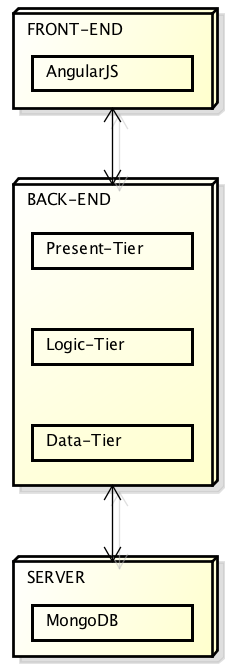
\includegraphics[height=0.6\textheight]{img/architettura_generale}
	\caption[Architettura generale del sistema]{Architettura generale del sistema}
\end{figure}

\textbf{Presentation-Tier}: contiene il front-end dell'applicazione, che si occupa della presentazione dei dati all'utente. Funge da interfaccia tra l'utente e il back-end, interagendo con il tier sottostante.

\textbf{Logic-Tier}: comunica con il livello superiore elaborando le richieste generate da esso e recuperando i dati dal livello inferiore. Questo strato è a sua volta organizzato con un'architettura three-tier per la gestione del back-end dell'applicazione.

\textbf{Data-tier}: questo livello è costituito dal database dell'applicazione ed è dove vengono memorizzate e recuperate le informazioni. Nel nostro caso il database è di tipo non relazionale.
\subsection{Interfaccia REST-like}
Si é scelto di utilizzare uno stile \gls{REST-like} per quanto riguarda l'interfaccia della componente \gls{back-end} dell'applicativo \PROGETTO, cioè basato sullo stile \gls{REST} ma modificato per permettere l'autenticazione e l'utilizzo di determinate operazioni. Più precisamente il comportamento dell'interfaccia con cui si accede agli elementi della collection può considerarsi \gls{REST} all'interno di una sessione utente, ovvero dall'operazione di login fino a quella di logout. Le motivazioni di tale scelta sono le seguenti:
\begin{itemize}
	\item Semplicità di utilizzo;
	\item Semplicità di integrazione con i \gls{framework} esistenti (\gls{Angular}.js);
	\item Indipendenza dal \gls{linguaggio di programmazione} utilizzato.
	\end{itemize}
	\gls{REST} utilizza un aggregato di dati con un nome (\gls{URI}) e una rappresentazione su cui é possibile invocare operazioni \gls{CRUD} tramite la seguente configurazione:
	
	\begin{table}[h]
		\begin{tabular}{|p{0.2\textwidth}|p{0.35\textwidth}|p{0.35\textwidth}|}
			\toprule
			
			\textbf{Risorsa} & \textbf{URI della collection} \smallbreak
			es. http://site.com/users  & \textbf{URI di un utente} \smallbreak
			es. http:/site.com/users/\{id\} \\
			
			\midrule
			\textbf{GET} & Fornisce informazioni sui membri della collection. & Fornisce una rappresentazione dell'elemento della collection indicato. \\ \midrule
			\textbf{PUT} & Non utilizzata. & Sostituisce l'elemento della collection indicato. Se non esiste lo crea. \\  \midrule
			\textbf{POST} & Crea un nuovo elemento nella collection. La \gls{URI} del nuovo elemento é generata in automatico e solitamente viene restituita dall'operazione. & Non utilizzata. \\ \midrule
			\textbf{DELETE} & Non utilizzata. & Cancella l'elemento della collection indicato.  \\ \midrule
			
			
			\end{tabular}\\
			\caption{Tabella configurazioni REST}
			
			\end{table}
			
Si é deciso di scegliere il formato \gls{JSON} come formato di rappresentazione dei dati poiché si integra perfettamente con i \gls{framework} utilizzati e con il linguaggio \gls{Javascript}.


\newpage

\section{Architettura Front-End}
\subsection{Premi::Front-End}
	\subsubsection*{Informazioni sul package}
		\begin{figure}[h]
			\centering
			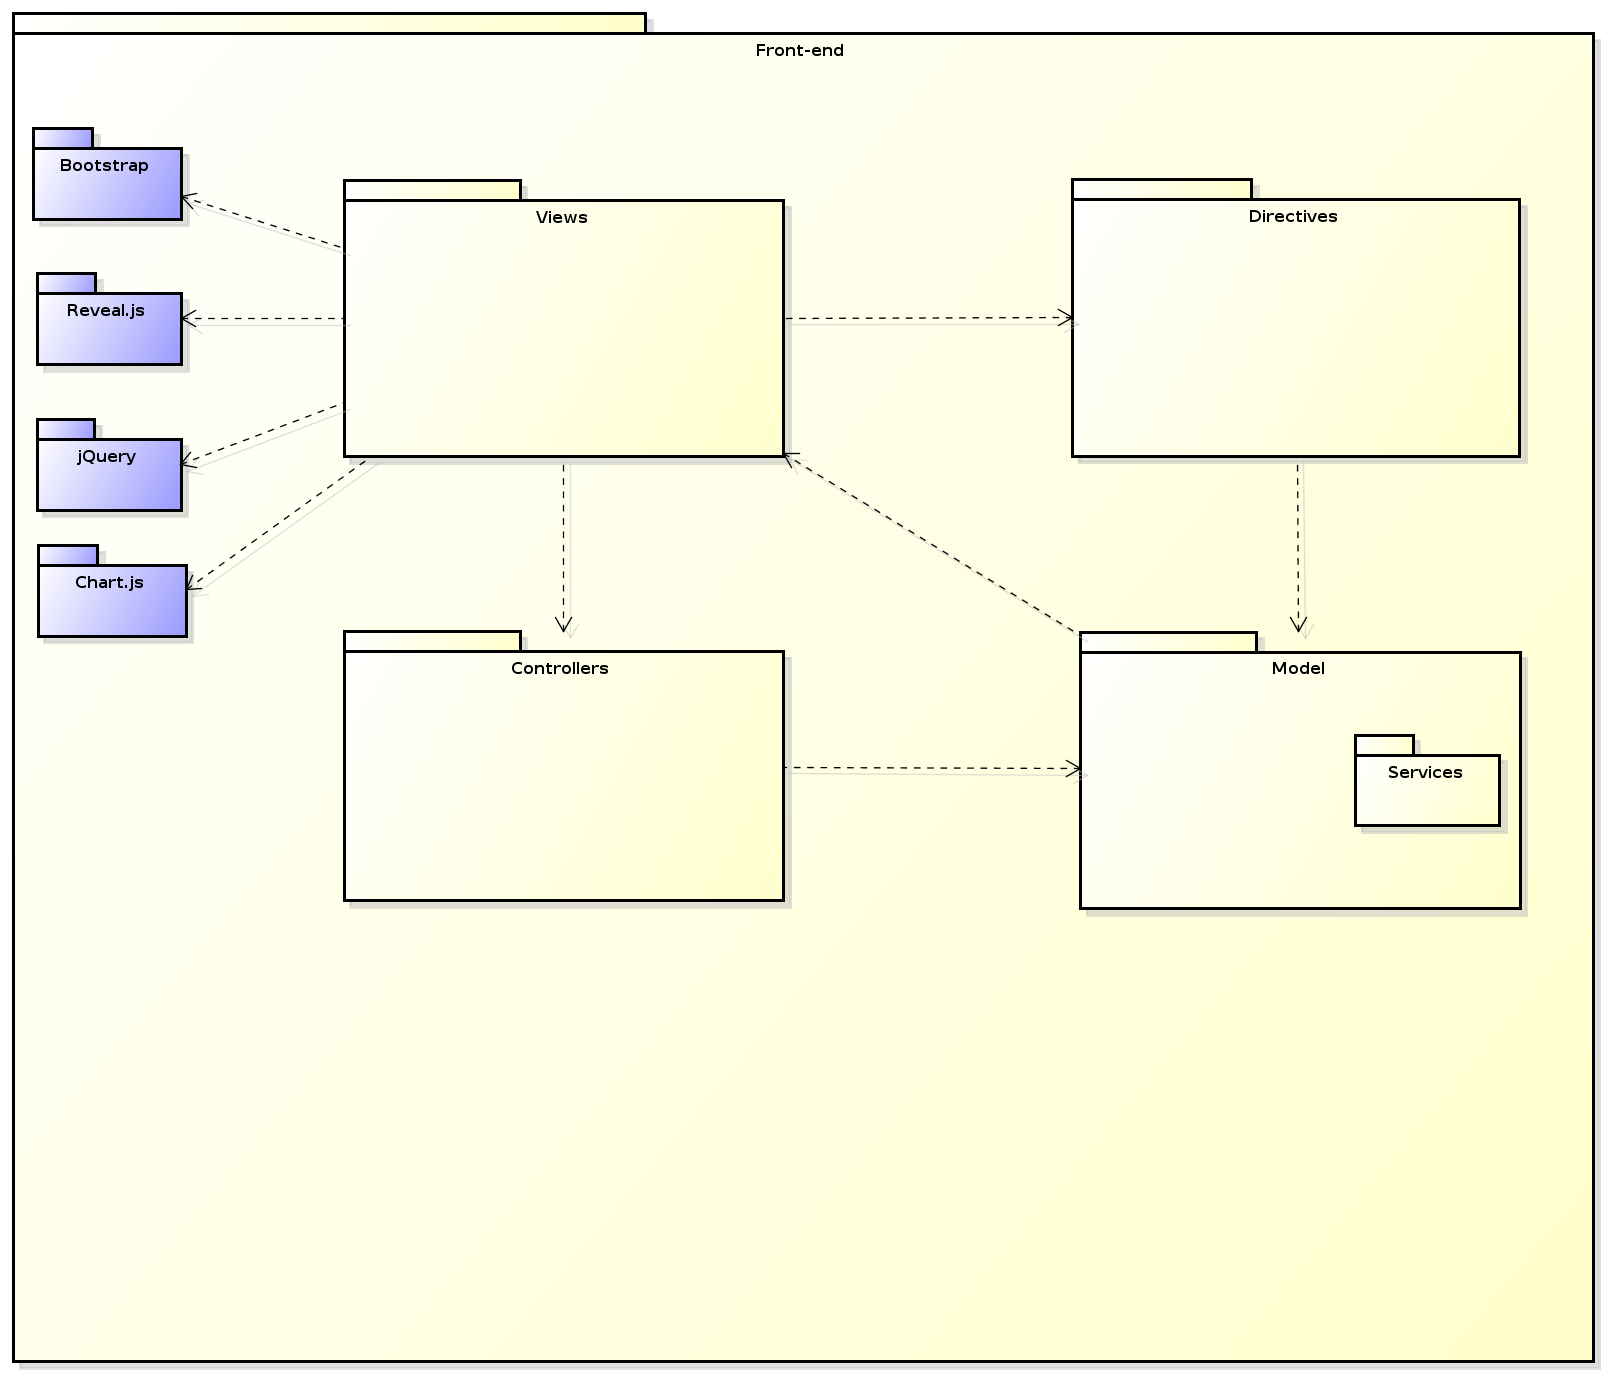
\includegraphics[width=0.7\linewidth]{img/front-end-package}
			\caption[Premi::Front-End]{Premi::Front-End}
		\end{figure}
		Il package contiene le varie componenti della parte di front-end dell'applicazione.

	\subsubsection*{Package contenuti:}
		\begin{itemize}
			\item \textbf{View:} Package contenente le views della componente front-end dell'applicazione;
			\item \textbf{Directives:} Package contenente le directives che compongono la view;
			\item \textbf{Model:} Package che definiscono la bussiness logic dell'applicazione;
			\item \textbf{Controller:} Package contenente i controller della parte front-end dell'applicazione.
		\end{itemize}


\subsection{Premi::Front-End::Model}
	\subsubsection*{Informazioni sul package}
		\begin{figure}[h]
			\centering
			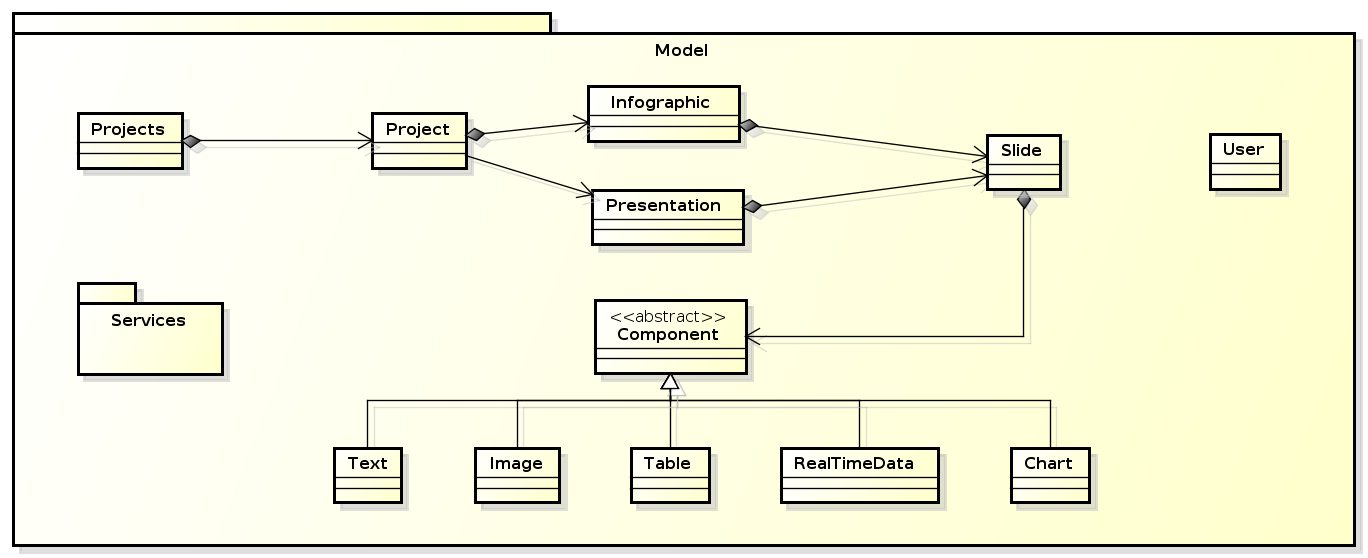
\includegraphics[width=0.7\linewidth]{img/front-end-package_model}
			\caption[Premi::Front-End::Model]{Premi::Front-End::Model}
		\end{figure}
		Il package serve per mantenere i dati relativi al \textit{front-end} e tutta la loro logica di business.

	\subsubsection*{Classi contenute:}
		\begin{itemize}
			
		 \item Premi::Front-End::Model::Projects:
			\begin{itemize}
				\item \textbf{Descrizione}:classe per la gestione di una collezione di progetti.Un progetto racchiude una presentazione e zero o più infografiche.
				\item \textbf{Relazioni con altre classi}:
				\begin{itemize}
					\item Premi::Front-End::Model::Project.
				\end{itemize}
			\end{itemize}
		
		\item Premi::Front-End::Model::Project: 
			 \begin{itemize}
				\item \textbf{Descrizione}: classe per la gestione di un progetto.
				\item \textbf{Relazioni con altre classi}:
				\begin{itemize}
					\item Premi::Front-End::Model::Presentation.
					\item Premi::Front-End::Model::Infographic.
				\end{itemize}
			\end{itemize}
		
		 \item Premi::Front-End::Model::Infographic:
			\begin{itemize}
				\item \textbf{Descrizione}: classe per la gestione di una infografica. Un'infografica ha il compito di raggruppare piu slide in un template grafico scelto dall'utente in un ordine impostabile di volta in volta.
				\item \textbf{Relazioni con altre classi}:
				\begin{itemize}
					\item Premi::Front-End::Model::Slide.
				\end{itemize}
			\end{itemize}
		 
		 \item Premi::Front-End::Model::Presentation:
			\begin{itemize}
				\item \textbf{Descrizione}: classe per la gestione di una presentazione. Una presentazione raggruppa più slide. Per la visualizzazione delle presentazioni è stato scelto di utilizzare il framework Reveal.js che permette di avere una visualizzazione a griglia, di conseguenza una presentazione deve memorizzare anche le coordinate delle sue slide.
				\item \textbf{Relazioni con altre classi}:
				\begin{itemize}
					\item Premi::Front-End::Model::Slide.
				\end{itemize}
			\end{itemize}

		 \item Premi::Front-End::Model::Slide: Classe per la gestione di una slide.
			\begin{itemize}
				\item \textbf{Descrizione}: classe per la gestione di una slide.
				\item \textbf{Relazioni con altre classi}:
				\begin{itemize}
					\item Premi::Front-End::Model::Component.
				\end{itemize}
			\end{itemize}
			
		 \item Premi::Front-End::Model::Component: 
			\begin{itemize}
				\item \textbf{Descrizione}: Classe astratta concretizzata ed estesa dalle varie componenti implementando il pattern \textit{composite} per fare si che elementi foglia e collezione vengano trattati allo stesso modo. Nello specifico, una tabella rappresenta un aggregato di altre componenti.
			\end{itemize}
			
		 \item Premi::Front-End::Model::Text:
			\begin{itemize}
				\item \textbf{Descrizione}: classe per la gestione di un elemento testuale e delle sue proprietà di formattazione. Concretizza ed estende Premi::Front-End::Model::Component.
				\item \textbf{Relazioni con altre classi}:
				\begin{itemize}
					\item Premi::Front-End::Model::Component.
				\end{itemize}
			\end{itemize}
			
		 \item Premi::Front-End::Model::Image:
			\begin{itemize}
				\item \textbf{Descrizione}: lasse per la gestione di un elemento di tipo immagine.
				\item \textbf{Relazioni con altre classi}:
				\begin{itemize}
					\item Premi::Front-End::Model::Component.
				\end{itemize}
			 \end{itemize}

		 \item Premi::Front-End::Model::Table:
			\begin{itemize}
				\item \textbf{Descrizione}: classe per la gestione di una tabella. Una tabella può contenere altre componenti che concretizzano la classe Premi::Front-End::Model::Component.
				\item \textbf{Relazioni con altre classi}:
				\begin{itemize}
					\item Premi::Front-End::Model::Component.
				\end{itemize}
			 \end{itemize}

		 \item Premi::Front-End::Model::RealTimeData:
			\begin{itemize}
				\item \textbf{Descrizione}: classe per la gestione di componenti che si aggiornano in tempo reale con cadenza personalizzabile.
				\item \textbf{Relazioni con altre classi}:
				\begin{itemize}
					\item Premi::Front-End::Model::Component.
				\end{itemize}
			 \end{itemize}
		
		 \item Premi::Front-End::Model::Chart: 
			\begin{itemize}
				\item \textbf{Descrizione}: classe per la gestione dei dati necessari per disegnare un grafico.
				\item \textbf{Relazioni con altre classi}:
				\begin{itemize}
					\item Premi::Front-End::Model::Component.
				\end{itemize}
			 \end{itemize}
		
		 \item Premi::Front-End::Model::User:
			\begin{itemize}
				\item \textbf{Descrizione}: classe per la gestione degli utenti.
			 \end{itemize}

		\end{itemize}
		
		
\subsection{Premi::Front-End::Views}
	\subsubsection*{Informazioni sul package}
		\begin{figure}[h]
			\centering
			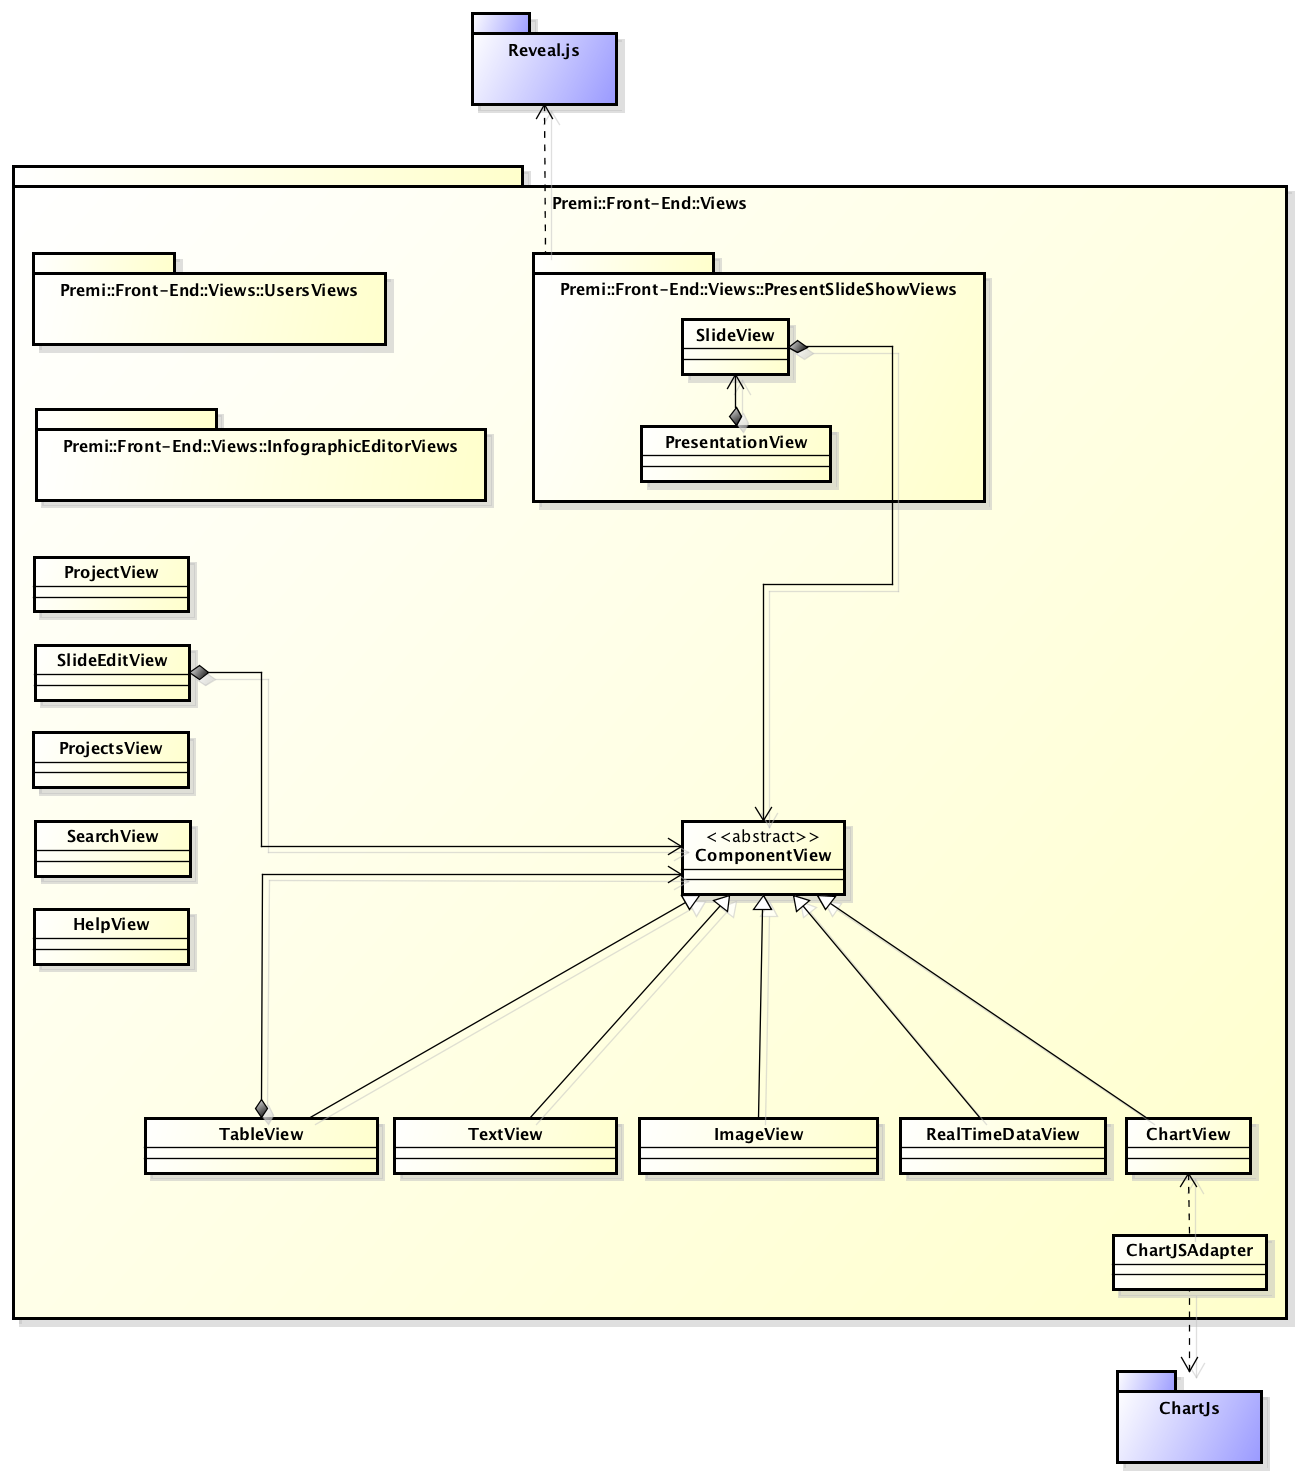
\includegraphics[width=0.7\linewidth]{img/front-end_views}
			\caption[Premi::Front-End::Views]{Premi::Front-End::Views}
		\end{figure}
		Il package contiene gli elementi per creare la parte grafica del front-end, la visualizzazione delle pagine e dell'editor del progetto.
	
	\subsubsection*{Package contenuti:}

	\begin{itemize}		
		\item Premi::Front-End::Views::UsersViews:
			\begin{itemize}
				\item \textbf{Descrizione}: classe per la gestione delle pagine riguardanti l'accesso al sito.
			\end{itemize}
		
		\item Premi::Front-End::Views::PresentSlideShowViews:
			\begin{itemize}
				\item \textbf{Descrizione}: classe per la gestione delle pagine per la visualizzazione della presentazione.
			\end{itemize}
		
		\item Premi::Front-End::Views::InfographicsEditorViews:
		\begin{itemize}
			\item \textbf{Descrizione}: classe per la gestione delle infografiche relative al progetto.
		\end{itemize}
	\end{itemize}
	
	\subsubsection*{Classi contenute:}
	\begin{itemize}
		
		\item Premi::Front-End::Views::UsersViews:
		\begin{itemize}
			\item \textbf{Descrizione}: classe per la gestione delle pagine riguardanti l'accesso al sito.
		\end{itemize}
		
		\item Premi::Front-End::Views::ProjectView:
		\begin{itemize}
			\item \textbf{Descrizione}: classe per la gestione della pagina del progetto attualmente aperto dall'utente.
		\end{itemize}
		
		\item Premi::Front-End::Views::SlideEditView:
		\begin{itemize}
			\item \textbf{Descrizione}: classe per la gestione della pagina dell'editor di una slide;
			\item \textbf{Relazioni con altre classi}:
			\begin{itemize}
				\item Premi::Front-End::Views::ComponentView.
			\end{itemize}
		\end{itemize}
		
		\item Premi::Front-End::Views::ProjectsView:
		\begin{itemize}
			\item \textbf{Descrizione}: classe per la gestione della pagina contenente i progetti creati da un utente.
		\end{itemize}
		
		\item Premi::Front-End::Views::SearchView:
		\begin{itemize}
			\item \textbf{Descrizione}: classe per la gestione della pagina per la ricerca di un progetto e la visualizzazione dei risultati.
		\end{itemize}
		
		\item Premi::Front-End::Views::HelpView:
		\begin{itemize}
			\item \textbf{Descrizione}: classe per la gestione della pagina della guida dell'applicazione.
		\end{itemize}
		
		\item Premi::Front-End::Views::ComponentView:
		\begin{itemize}
			\item \textbf{Descrizione}: classe base per la gestione grafica degli elementi che è possibile includere in una slide.
		\end{itemize}
		
		\item Premi::Front-End::Views::TableView:
		\begin{itemize}
			\item \textbf{Descrizione}: classe per la gestione grafica dell'elemento tabella che è possibile includere in una slide. Può essere composta da altri elementi della classe *::ComponentView;
			\item \textbf{Relazioni con altre classi}:
			\begin{itemize}
				\item Premi::Front-End::Views::ComponentView.
			\end{itemize}
		\end{itemize}
		
		
		\item Premi::Front-End::Views::TextView:
		\begin{itemize}
			\item \textbf{Descrizione}: classe per la gestione grafica dell'elemento casella di testo che è possibile includere in una slide;
			\item \textbf{Relazioni con altre classi}:
			\begin{itemize}
				\item Premi::Front-End::Views::ComponentView.
			\end{itemize}
		\end{itemize}
		
		\item Premi::Front-End::Views::ImageView:
		\begin{itemize}
			\item \textbf{Descrizione}: classe per la gestione grafica dell'elemento immagine che è possibile includere in una slide;
			\item \textbf{Relazioni con altre classi}:
			\begin{itemize}
				\item Premi::Front-End::Views::ComponentView.
			\end{itemize}
		\end{itemize}
		
		\item Premi::Front-End::Views::RealTimeDataView:
		\begin{itemize}
			\item \textbf{Descrizione}: classe per la gestione grafica dell'elemento di dati real-time che è possibile includere in una slide;
			\item \textbf{Relazioni con altre classi}:
			\begin{itemize}
				\item Premi::Front-End::Views::ComponentView.
			\end{itemize}
		\end{itemize}
		
		\item Premi::Front-End::Views::ChartView:
		\begin{itemize}
			\item \textbf{Descrizione}: classe per la gestione grafica dell'elemento grafico che è possibile includere in una slide;
			\item \textbf{Relazioni con altre classi}:
			\begin{itemize}
				\item Premi::Front-End::Views::ComponentView;
				\item Premi::Front-End::Views::ChartJsAdapter;
			\end{itemize}
		\end{itemize}
		
		\item Premi::Front-End::Views::ChartJsAdapter:
		\begin{itemize}
			\item \textbf{Descrizione}: classe per interfacciare l'utilizzo della classe Chart.Js con la classe ChartView;
			\item \textbf{Relazioni con altre classi}:
			\begin{itemize}
				\item Premi::Front-End::Views::ChartView;
			\end{itemize}
			\item \textbf{Relazioni con altri package}:
			\begin{itemize}
				\item Chart.Js
			\end{itemize}
		\end{itemize}
	\end{itemize}
	
	
\subsection{Premi::Front-End::Views::UsersViews}
	\subsubsection*{Informazioni sul package}
	\begin{figure}[h]
		\centering
		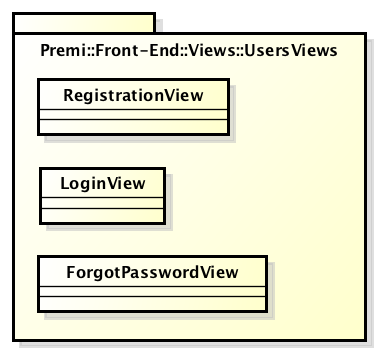
\includegraphics[width=0.7\linewidth]{img/front-end_views_usersviews}
		\caption[Premi::Front-End::Views::UsersViews]{Premi::Front-End::Views::UsersViews}
	\end{figure}
	Il package contiene le classi per creare la parte grafica dell'accesso di un utente all'applicazione.
	
	\subsubsection*{Classi contenute:}
	\begin{itemize}
		
		\item Premi::Front-End::Views::UsersViews::RegistrationView:
		\begin{itemize}
			\item \textbf{Descrizione}: classe per creare la sezione relativa alla registrazione di un nuovo utente.
		\end{itemize}
		
		\item Premi::Front-End::Views::UsersViews::LoginView:
		\begin{itemize}
			\item \textbf{Descrizione}: classe per creare la sezione relativa al login di utente già registrato.
		\end{itemize}
		
		\item Premi::Front-End::Views::UsersViews::ForgotPasswordView:
		\begin{itemize}
			\item \textbf{Descrizione}: classe per creare la sezione relativa al recupero della password per l'utente registrato.
		\end{itemize}
	\end{itemize}
	
	
\subsection{Premi::Front-End::Views::PresentSlideShowViews}
	\subsubsection*{Informazioni sul package}
	\begin{figure}[h]
		\centering
		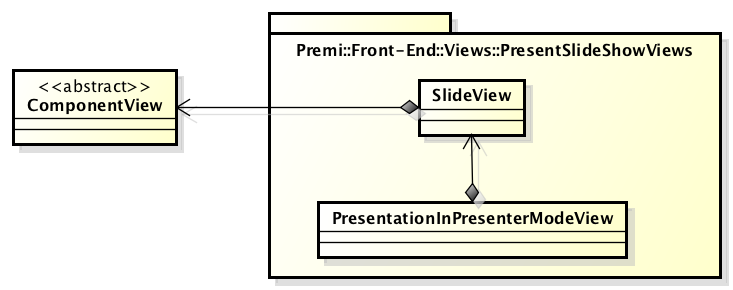
\includegraphics[width=0.7\linewidth]{img/front-end_views_presentslideshowviews}
		\caption[Premi::Front-End::Views::PresentSlideShowViews]{Premi::Front-End::Views::PresentSlideShowViews}
	\end{figure}
	Il package contiene le classi per la parte grafica relativa alla visualizzazione della presentazione da parte dell'utente.
	
	\subsubsection*{Classi contenute:}
		\begin{itemize}
			\item Premi::Front-End::Views::PresentSlideShowViews::SlideView:
			\begin{itemize}
				\item \textbf{Descrizione}: classe per creare la parte grafica di una slide nella visualizzazione di una presentazione. È composta da oggetti della classe ComponentView,o sue derivate;
				\item \textbf{Relazioni con altre classi}:
				\begin{itemize}
					\item Premi::Front-End::Views::ComponentView.
				\end{itemize}
			\end{itemize}
			
			\item Premi::Front-End::Views::PresentSlideShowViews::PresentationInPresenterModeView:
			\begin{itemize}
				\item \textbf{Descrizione}: classe per creare la parte grafica di una slide nella visualizzazione di una presentazione nella modalità presentatore. È composta da oggetti della classe SlideView in quanto la contiene implementandola;
				\item \textbf{Relazioni con altre classi}:
				\begin{itemize}
					\item Premi::Front-End::Views::PresentSlideShowViews::SlideView.
				\end{itemize}
			\end{itemize}
		\end{itemize}
		
\subsection{Premi::Front-End::Views::InfographicEditorViews}
	\subsubsection*{Informazioni sul package}
	\begin{figure}[h]
		\centering
		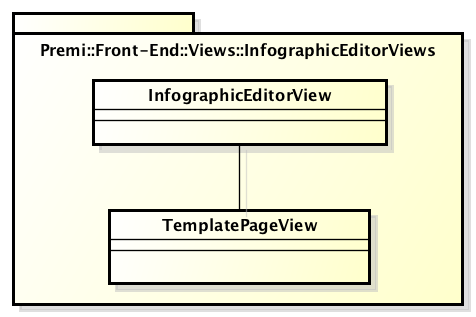
\includegraphics[width=0.7\linewidth]{img/front-end_views_infographiceditorviews}
		\caption[Premi::Front-End::Views::InfographicEditorViews]{Premi::Front-End::Views::InfographicEditorViews}
	\end{figure}
	Il package contiene le classi per la parte grafica relativa alle infografiche e alla loro creazione.

	\subsubsection*{Classi contenute:}
	\begin{itemize}
		
		\item Premi::Front-End::Views::InfographicEditorViews::InfographicEditorView:
		\begin{itemize}
			\item \textbf{Descrizione}: classe per creare un'infografica. Permette la personalizzazione di essa attraverso la selezione delle slide da usare.
		\end{itemize}
		
		\item Premi::Front-End::Views::InfographicEditorViews::TemplatePageView:
		\begin{itemize}
			\item \textbf{Descrizione}: classe che permette di creare la sezione per selezionare il template da utilizzare nell'infografica;
			\item \textbf{Relazioni con altre classi}:
			\begin{itemize}
				\item Premi::Front-End::Views::InfographicEditorViews::InfographicEditorView.
			\end{itemize}
		\end{itemize}
	\end{itemize}


\newpage

\section{Architettura Back-End}
\subsection{Interfaccia REST}
Di seguito sono elencate le risorse \gls{REST} associate al tipo di metodo che è possibile richiedere su di esse e i permessi richiesti per poter effettuare la richiesta.
Le tipologie di permessi sono:
\begin{itemize}
	\item Utente non autenticato: risorsa che può essere richiesta da qualsiasi utente;
	\item Utente autenticato: risorsa che può essere richiesta solo da utenti autenticati;
	\item Utente proprietario: risorsa che può essere richiesta solo da utenti proprietari di un progetto. Un utente proprietario della sua collection di progetti é anche proprietario degli altri elementi contenuti nella collection.
\end{itemize}

\begin{table}[h]
	\begin{tabular}{|p{0.5\textwidth}|p{0.15\textwidth}|p{0.35\textwidth}|}
		\toprule
		
		\textbf{Chiamata} & \textbf{Tipo risorsa}  & \textbf{Tipo utente} \\
		\bottomrule
	\end{tabular}\\	
\end{table}

\begin{table}[h]
	\begin{tabular}{|p{0.5\textwidth}|p{0.15\textwidth}|p{0.35\textwidth}|}
		\toprule
		\textbf{/auth/register} & \textbf{POST} & \textbf{Utente non autenticato} \\ \midrule
		\multicolumn{3}{|c|}{Crea una richiesta di registrazione.} \\
		\bottomrule
	\end{tabular}\\
	\par\bigskip
	
	\begin{tabular}{|p{0.5\textwidth}|p{0.15\textwidth}|p{0.35\textwidth}|}
		\toprule
		\textbf{/auth/login} & \textbf{POST} & \textbf{Utente non autenticato} \\ \midrule
		\multicolumn{3}{|c|}{Crea una richiesta di autenticazione.} \\
		\bottomrule
	\end{tabular}\\
	\par\bigskip
	
	\begin{tabular}{|p{0.5\textwidth}|p{0.15\textwidth}|p{0.35\textwidth}|}
		\toprule
		\textbf{/auth/logout} & \textbf{POST} & \textbf{Utente autenticato} \\ \midrule
		\multicolumn{3}{|c|}{Crea una richiesta di disconnessione.} \\
		\bottomrule
	\end{tabular}\\
	\par\bigskip
	
	\begin{tabular}{|p{0.5\textwidth}|p{0.15\textwidth}|p{0.35\textwidth}|}
		\toprule
		\textbf{/api/user} & \textbf{GET} & \textbf{Utente autenticato} \\ \midrule
		\multicolumn{3}{|c|}{Restituisce le informazioni relative all'utente corrente.} \\
		\bottomrule
	\end{tabular}\\
	\par\bigskip
	
	\begin{tabular}{|p{0.5\textwidth}|p{0.15\textwidth}|p{0.35\textwidth}|}
		\toprule
		\textbf{/api/user} & \textbf{POST} & \textbf{Utente autenticato} \\ \midrule
		\multicolumn{3}{|c|}{Inserisce le informazioni relative all'utente corrente.} \\
		\bottomrule
	\end{tabular}\\
	\par\bigskip
	
	\begin{tabular}{|p{0.5\textwidth}|p{0.15\textwidth}|p{0.35\textwidth}|}
		\toprule
		\textbf{/api/user/\{user\}} & \textbf{GET} & \textbf{Utente non autenticato, Utente autenticato} \\ \midrule
		\multicolumn{3}{|c|}{Restituisce le informazioni relative all'utente {user}.} \\
		\bottomrule
	\end{tabular}\\
	\par\bigskip
	
	\begin{tabular}{|p{0.5\textwidth}|p{0.15\textwidth}|p{0.35\textwidth}|}
		\toprule
		\textbf{/api/user/\{user\}} & \textbf{PUT} & \textbf{Utente autenticato} \\ \midrule
		\multicolumn{3}{|c|}{Aggiorna le informazioni relative all'utente \{user\}.} \\
		\bottomrule
	\end{tabular}\\
	\par\bigskip
		
	\begin{tabular}{|p{0.5\textwidth}|p{0.15\textwidth}|p{0.35\textwidth}|}
		\toprule
		\textbf{/api/user/\{user\}} & \textbf{DELETE} & \textbf{Utente autenticato} \\ \midrule
		\multicolumn{3}{|c|}{Rimuove dal sistema l'utente \{user\}.} \\
		\bottomrule
	\end{tabular}\\
	\par\bigskip
	
	
\end{table}
\newpage	
\begin{table}[H]	
		
	\begin{tabular}{|p{0.5\textwidth}|p{0.15\textwidth}|p{0.35\textwidth}|}
		\toprule
		\textbf{/api/user/\{user\}/project} & \textbf{GET} & \textbf{Utente non autenticato, Utente autenticato, Utente proprietario} \\ \midrule
		\multicolumn{3}{|c|}{Restituisce i progetti dell'utente \{user\}.} \\
		\bottomrule
	\end{tabular}\\
	\par\bigskip
	
	\begin{tabular}{|p{0.5\textwidth}|p{0.15\textwidth}|p{0.35\textwidth}|}
		\toprule
		\textbf{/api/user/\{user\}/project} & \textbf{POST} & \textbf{Utente autenticato} \\ \midrule
		\multicolumn{3}{|c|}{Crea un nuovo progetto di proprietà dell'utente \{user\}.} \\
		\bottomrule
	\end{tabular}\\
	\par\bigskip
	
	\begin{tabular}{|p{0.5\textwidth}|p{0.15\textwidth}|p{0.35\textwidth}|}
		\toprule
		\textbf{/api/user/\{user\}/project/\{project\}} & \textbf{GET} & \textbf{Utente non autenticato, Utente autenticato, Utente proprietario} \\ \midrule
		\multicolumn{3}{|c|}{Restituisce il progetto \{project\} dell'utente \{user\}.} \\
		\bottomrule
	\end{tabular}\\
	\par\bigskip
	
	\begin{tabular}{|p{0.5\textwidth}|p{0.15\textwidth}|p{0.35\textwidth}|}
		\toprule
		\textbf{/api/user/\{user\}/project/\{project\}} & \textbf{PUT} & \textbf{Utente proprietario} \\ \midrule
		\multicolumn{3}{|c|}{Aggiorna il progetto \{project\} dell'utente \{user\}.} \\
		\bottomrule
	\end{tabular}\\
	\par\bigskip

	\begin{tabular}{|p{0.5\textwidth}|p{0.15\textwidth}|p{0.35\textwidth}|}
		\toprule
		\textbf{/api/user/\{user\}/project/\{project\}} & \textbf{DELETE} & \textbf{Utente proprietario} \\ \midrule
		\multicolumn{3}{|c|}{Elimina il progetto \{project\} dell'utente \{user\}.} \\
		\bottomrule
	\end{tabular}\\
	\par\bigskip
	
	\begin{tabular}{|p{0.5\textwidth}|p{0.15\textwidth}|p{0.35\textwidth}|}
		\toprule
		\textbf{/api/user/\{user\}/project/\{project\}
		/infographic} & \textbf{GET} & \textbf{Utente non autenticato, Utente autenticato, Utente proprietario} \\ \midrule
		\multicolumn{3}{|c|}{Restituisce tutte le infografiche del progetto \{project\} dell'utente \{user\}.} \\
		\bottomrule
	\end{tabular}\\
	\par\bigskip
	
	\begin{tabular}{|p{0.5\textwidth}|p{0.15\textwidth}|p{0.35\textwidth}|}
		\toprule
		\textbf{/api/user/\{user\}/project
		/infographic} & \textbf{POST} & \textbf{Utente autenticato} \\ \midrule
		\multicolumn{3}{|c|}{Crea un'infografica nel progetto \{project\} dell'utente \{user\}.} \\
		\bottomrule
	\end{tabular}\\
	
	\begin{tabular}{|p{0.5\textwidth}|p{0.15\textwidth}|p{0.35\textwidth}|}
		\toprule
		\textbf{/api/user/\{user\}/project/\{project\}
		/infographic/\{infographic\}} & \textbf{GET} & \textbf{Utente non autenticato, Utente autenticato, Utente proprietario} \\ \midrule
		\multicolumn{3}{|c|}{Restituisce l'infografica \{infographic\} tra quelle del  progetto \{project\} dell'utente \{user\}.} \\
		\bottomrule
	\end{tabular}\\
	\par\bigskip
	
	\begin{tabular}{|p{0.5\textwidth}|p{0.15\textwidth}|p{0.35\textwidth}|}
		\toprule
		\textbf{/api/user/\{user\}/project/\{project\}
		/infographic/\{infographic\}} & \textbf{PUT} & \textbf{Utente proprietario} \\ \midrule
		\multicolumn{3}{|c|}{Aggiorna l'infografica \{infographic\} tra quelle del progetto \{project\} dell'utente \{user\}.} \\
		\bottomrule
	\end{tabular}\\
	\par\bigskip
	
	\begin{tabular}{|p{0.5\textwidth}|p{0.15\textwidth}|p{0.35\textwidth}|}
		\toprule
		\textbf{/api/user/\{user\}/project/\{project\}
		/infographic/\{infographic\}} & \textbf{DELETE} & \textbf{Utente proprietario} \\ \midrule
		\multicolumn{3}{|c|}{Elimina l'infografica \{infographic\} tra quelle del progetto \{project\} dell'utente \{user\}.} \\
		\bottomrule
	\end{tabular}\\
	\par\bigskip
		
\end{table}
\newpage



\begin{table}[H]
	\begin{tabular}{|p{0.5\textwidth}|p{0.15\textwidth}|p{0.35\textwidth}|}
		\toprule
		\textbf{/api/user/\{user\}/project/\{project\}
		/presentation/} & \textbf{POST} & \textbf{Utente autenticato} \\ \midrule
		\multicolumn{3}{|c|}{Crea la presentazione del progetto \{project\} dell'utente \{user\}.} \\
		\bottomrule
	\end{tabular}\\
	\par\bigskip

	\begin{tabular}{|p{0.5\textwidth}|p{0.15\textwidth}|p{0.35\textwidth}|}
		\toprule
		\textbf{/api/user/\{user\}/project/\{project\}
		/presentation/\{presentation\}} & \textbf{GET} & \textbf{Utente non autenticato, Utente autenticato, Utente proprietario} \\ \midrule
		\multicolumn{3}{|c|}{Restituisce la presentazione \{presentation\} del progetto \{project\} dell'utente \{user\}.} \\
		\bottomrule
	\end{tabular}\\
	\par\bigskip
	
	\begin{tabular}{|p{0.5\textwidth}|p{0.15\textwidth}|p{0.35\textwidth}|}
		\toprule
		\textbf{/api/user/\{user\}/project/\{project\}
		/presentation/\{presentation\}} & \textbf{PUT} & \textbf{Utente proprietario} \\ \midrule
		\multicolumn{3}{|c|}{Aggiorna la presentazione \{presentation\} del progetto \{project\} dell'utente \{user\}.} \\
		\bottomrule
	\end{tabular}\\
	\par\bigskip
	
	\begin{tabular}{|p{0.5\textwidth}|p{0.15\textwidth}|p{0.35\textwidth}|}
		\toprule
		\textbf{/api/user/\{user\}/project/\{project\}
		/presentation/\{presentation\}} & \textbf{DELETE} & \textbf{Utente proprietario} \\ \midrule
		\multicolumn{3}{|c|}{Elimina la presentazione \{presentation\} del progetto \{project\} dell'utente \{user\}.} \\
		\bottomrule
	\end{tabular}\\
	\par\bigskip
	
	
	
	
	
	
	
	
	
	
	
	
	\begin{tabular}{|p{0.5\textwidth}|p{0.15\textwidth}|p{0.35\textwidth}|}
		\toprule
		\textbf{/api/user/\{user\}/project/\{project\}
		/presentation/\{presentation\}/slide} & \textbf{GET} & \textbf{Utente non autenticato, Utente autenticato, Utente proprietario} \\ \midrule
		\multicolumn{3}{|c|}{Restituisce tutte le slide della presentazione \{presentation\} del progetto \{project\} dell'utente \{user\}.} \\
		\bottomrule
	\end{tabular}\\
	\par\bigskip
	
	\begin{tabular}{|p{0.5\textwidth}|p{0.15\textwidth}|p{0.35\textwidth}|}
		\toprule
		\textbf{/api/user/\{user\}/project/\{project\}
		/presentation/\{presentation\}/slide/\{slide\}} & \textbf{GET} & \textbf{Utente autenticato} \\ \midrule
		\multicolumn{3}{|c|}{Restituisce la slide  \{slide\} della presentazione \{presentation\} del progetto \{project\} dell'utente \{user\}.} \\
		\bottomrule
	\end{tabular}\\
	\par\bigskip
	
	\begin{tabular}{|p{0.5\textwidth}|p{0.15\textwidth}|p{0.35\textwidth}|}
		\toprule
		\textbf{/api/user/\{user\}/project/\{project\}
		/presentation/\{presentation\}/slide} & \textbf{POST} & \textbf{Utente proprietario} \\ \midrule
		\multicolumn{3}{|c|}{Crea una slide della presentazione \{presentation\} del progetto \{project\} dell'utente \{user\}.} \\
		\bottomrule
	\end{tabular}\\
	\par\bigskip
	
	\begin{tabular}{|p{0.5\textwidth}|p{0.15\textwidth}|p{0.35\textwidth}|}
		\toprule
		\textbf{/api/user/\{user\}/project/\{project\}
		/presentation/\{presentation\}/slide/\{slide\}} & \textbf{PUT} & \textbf{Utente autenticato} \\ \midrule
		\multicolumn{3}{|c|}{Aggiorna la slide \{slide\} della presentazione \{presentation\} del progetto \{project\} dell'utente \{user\}.} \\
		\bottomrule
	\end{tabular}\\
	\par\bigskip
	
	\begin{tabular}{|p{0.5\textwidth}|p{0.15\textwidth}|p{0.35\textwidth}|}
		\toprule
		\textbf{/api/user/\{user\}/project/\{project\}
		/presentation/\{presentation\}/slide/\{slide\}} & \textbf{DELETE} & \textbf{Utente autenticato} \\ \midrule
		\multicolumn{3}{|c|}{Elimina la \{slide\} slide della presentazione \{presentation\} del progetto \{project\} dell'utente \{user\}.} \\
		\bottomrule
	\end{tabular}\\
	\par\bigskip
	
	

\end{table}

\newpage

\subsection{Back-End}
	\subsubsection*{Informazioni sul package}
		\begin{figure}[h]
			\centering
			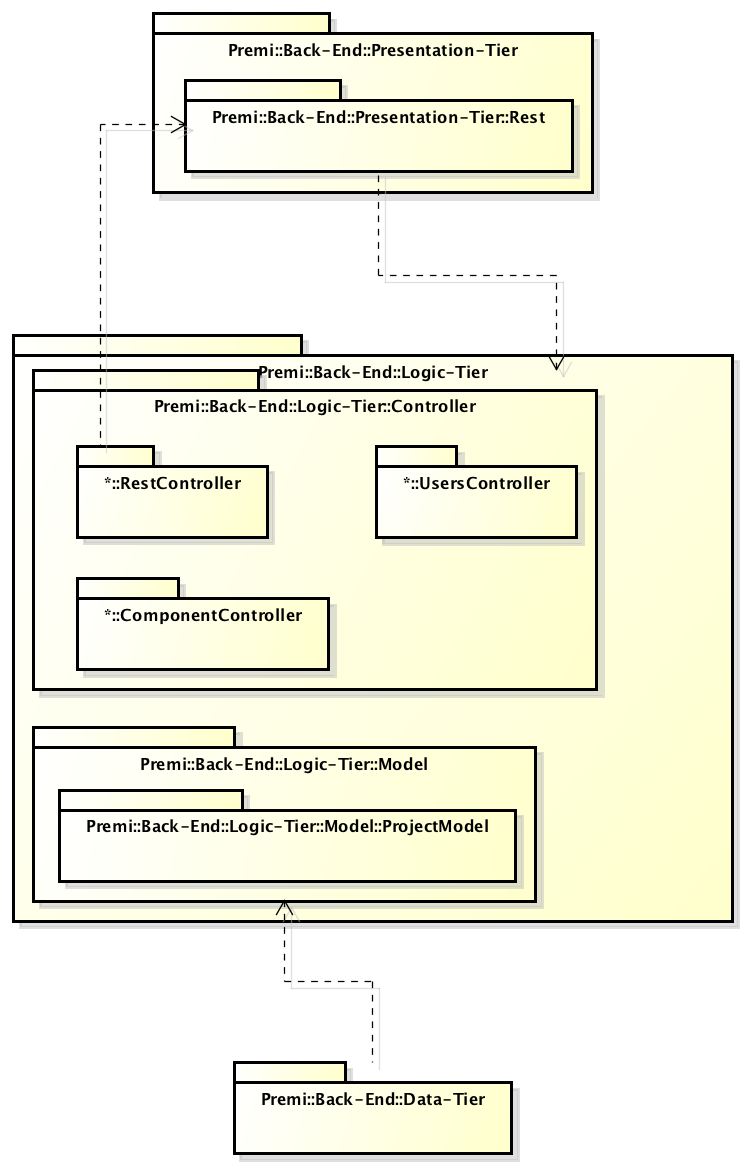
\includegraphics[width=0.9\linewidth]{img/back-end_package}
			\caption[Premi::Back-End]{Premi - Architettura di Back-End}
		\end{figure}
		Il package contiene le componenti della parte di \gls{back-end} dell'applicazione.
		
	\subsubsection*{Package contenuti}
		\begin{itemize}
			\item Premi::Presentation-Tier;
			\item Premi::Http;
			\item Premi::Model;
			\item Premi::Data-Tier.
		\end{itemize}

\newpage

\subsection{Premi::Presentation-Tier}
	\subsubsection*{Informazioni sul package}
		\begin{figure}[h]
			\centering
			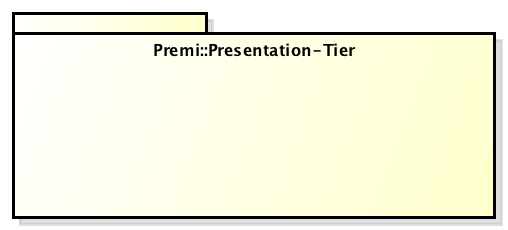
\includegraphics[width=0.5\linewidth]{img/premi_presentation-tier}
			\caption[Premi::Presentation-Tier]{Premi::Presentation-Tier}
		\end{figure}
		Il package rende possibile l'interfacciamento con il \gls{front-end}. Comunica con altri livelli attraverso i risultati di output al livello browser/client e tutti gli altri livelli della rete.
		Gestisce le chiamate \gls{REST} restituendo i risultati o eseguendo le procedure a seguito delle chiamate da parte del \gls{front-end} di uno specifico \gls{URI}. 
		
\newpage
		
\subsection{Logic Tier}
	\begin{figure}[h]
		\centering
		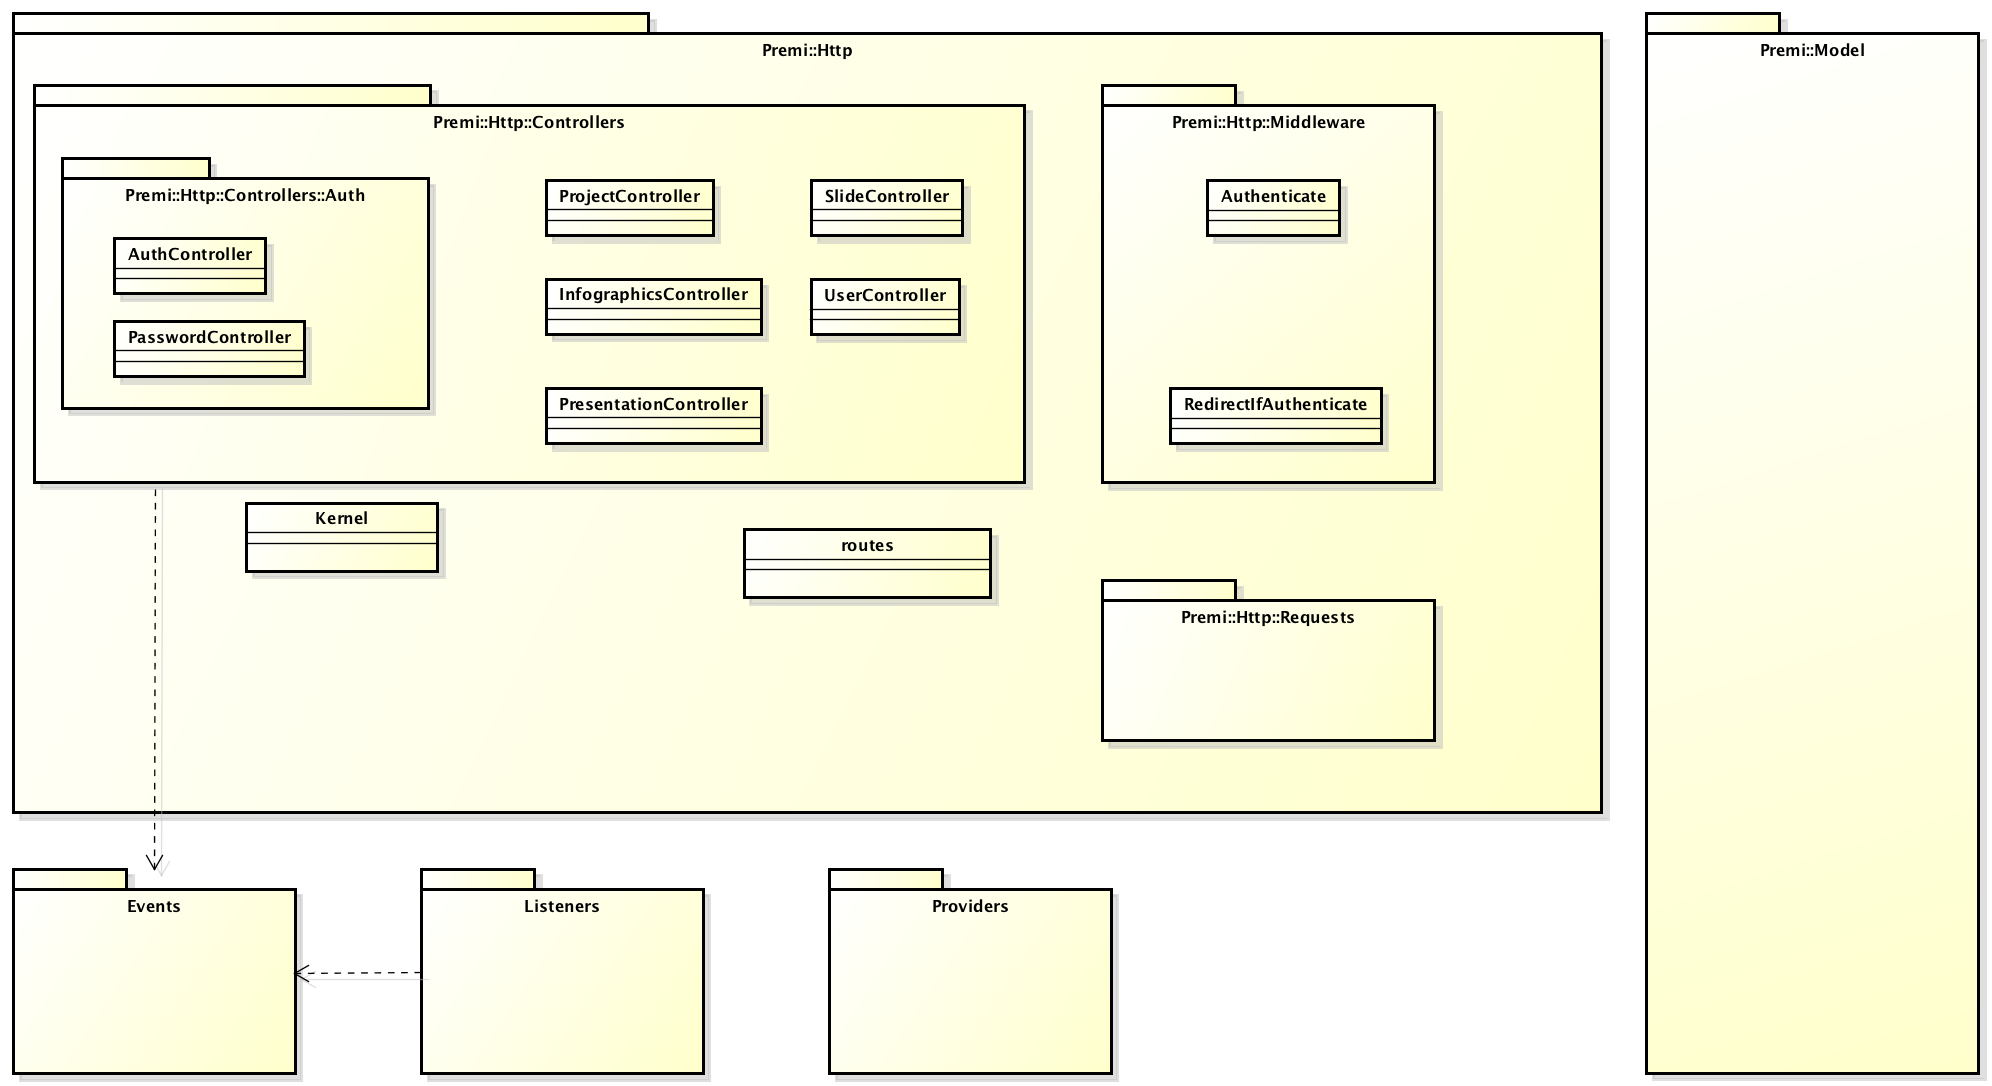
\includegraphics[width=\linewidth]{img/back-end_logic-tier_package}
		\caption[Premi::Http , Premi::Model]{Premi::Http , Premi::Model}
	\end{figure}
	Il core dell'applicazione viene implementato dal Model, che incapsulando lo stato dell'applicazione definisce i dati e le operazioni che possono essere eseguite su questi. Il package Http contiene Il componente Controller che ha la responsabilità di trasformare le interazioni dell'utente in azioni eseguite dal Model.
	
	\subsubsection*{Package contenuti}
	\begin{itemize}
		\item Premi::Http;
		\item Premi::Model.
	\end{itemize}

\newpage
\subsection{Premi::Http}
		\begin{figure}[h]
			\centering
			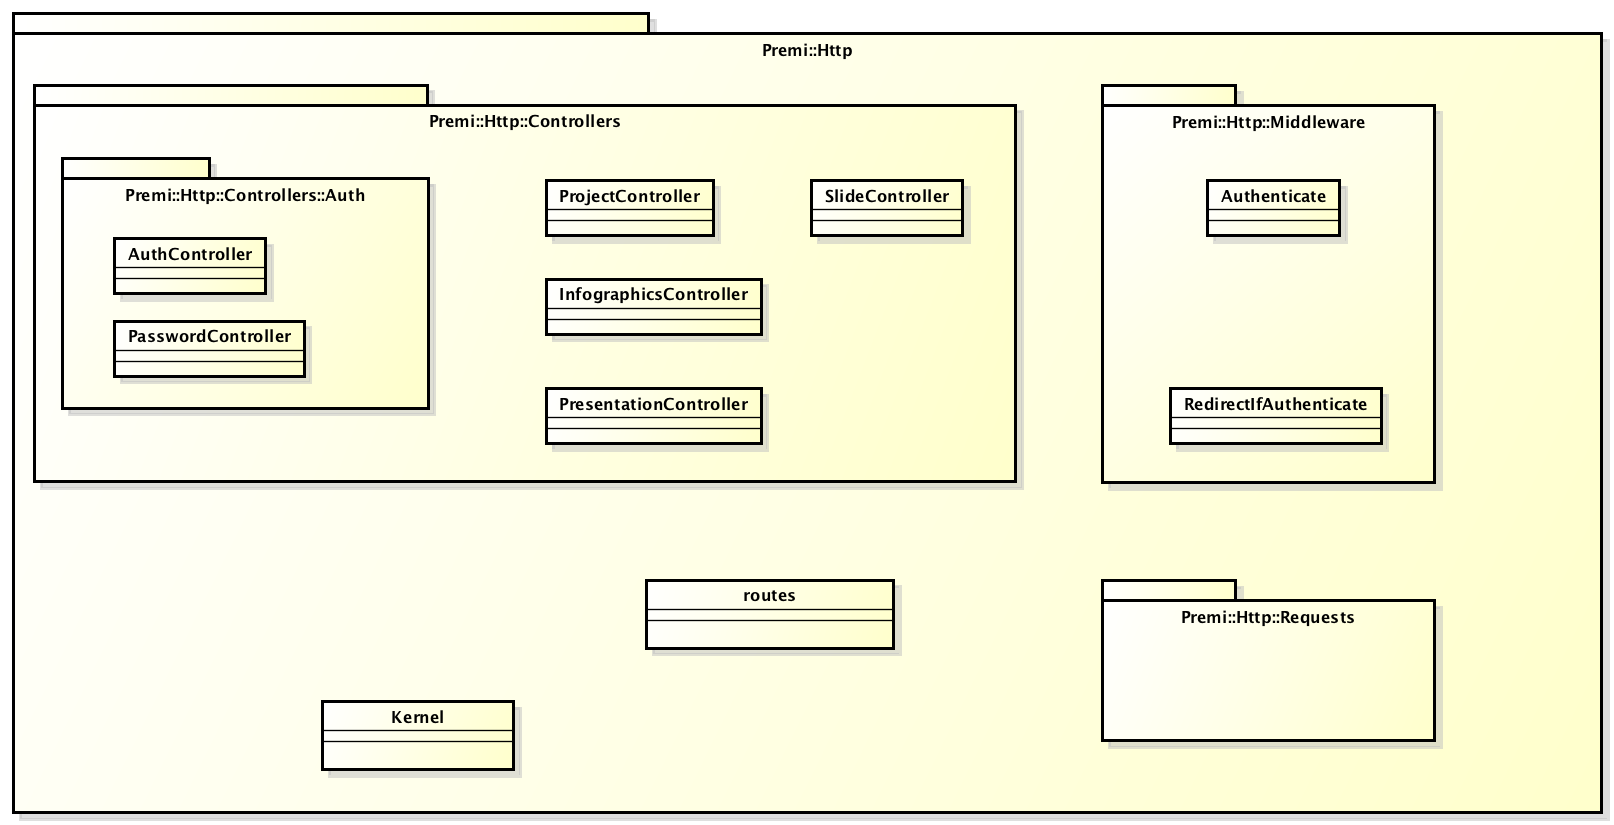
\includegraphics[width=0.9\linewidth]{img/premi_http}
			\caption[Premi::Http]{Premi::Http}
			\label{fig:premi_http}
		\end{figure}

	\subsubsection*{Informazioni sul package}
	 Il logic tier contiene a sua volta svariati package. Il package Http funziona come un'interfaccia alla vera applicazione.
	 \subsubsection*{Classi contenute}
	 \begin{itemize}
	 	\item \textbf{Routes: }collega una specifica richiesta ad un set di istruzioni ben precise;
	 	\item \textbf{Kernel: }"filtro" attraverso cui passano tutte le richieste.
	 \end{itemize}
	 \subsubsection*{Package contenuti}
		 \begin{itemize}
		 	\item Premi::Http::Controllers;
		 	\item Premi::Http::Middleware;
		 	\item Premi::Http::Requests;
		 \end{itemize}

\newpage
\subsection{Premi::Http::Controllers}
	\subsubsection*{Informazioni sul package}
	\begin{figure}[h]
		\centering
		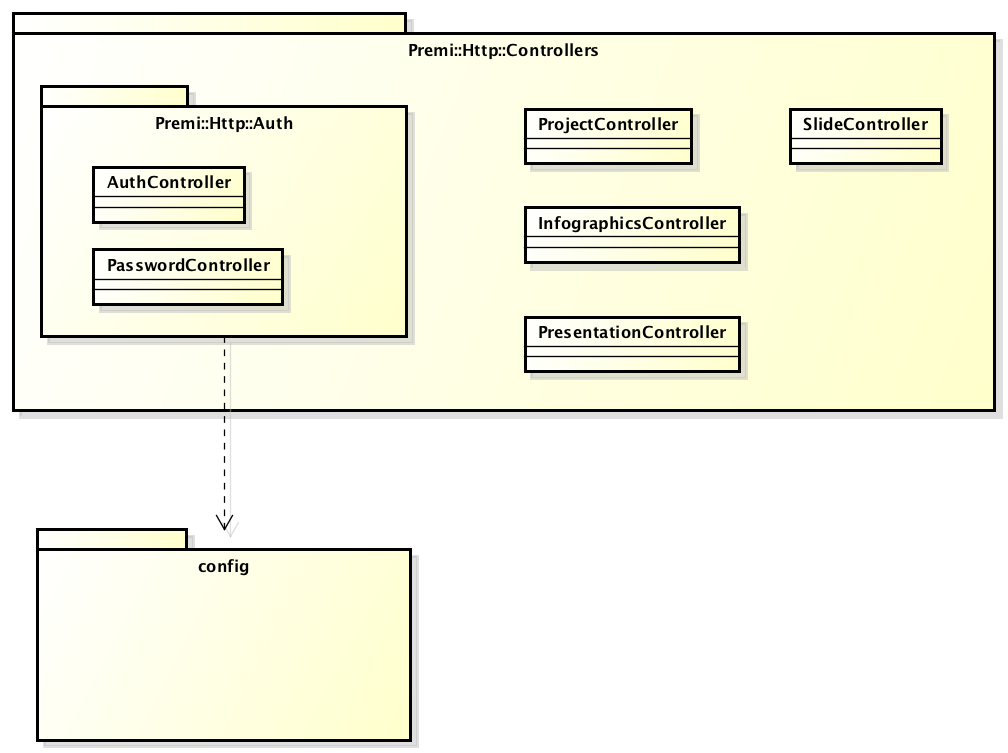
\includegraphics[width=0.9\linewidth]{img/premi_http_controllers}
		\caption[Premi::Http::Controllers]{Premi::Http::Controllers}
	\end{figure}
	Il package contiene le componenti che gestiscono la parte controller del lato \gls{back-end} dell'applicazione. 
	Sono presenti i controller per il progetto e i suoi componenti. È presente inoltre il package Auth che gestisce la parte di registrazione, autenticazione e recupero password dell'utente. 

	\subsubsection*{Package contenuti}
		\begin{itemize}
			\item Premi::Http::Controllers::Auth
		\end{itemize}
	\subsubsection*{Classi contenute}
		\begin{itemize}
			\item Premi::Http::Controllers::ProjectController;
			\item Premi::Http::Controllers::InfographicController;
			\item Premi::Http::Controllers::Presentation;
			\item Premi::Http::Controllers::SlideController.
		\end{itemize}
		
	
	\subsubsection*{Premi::Http::Controllers::Auth}
		\subsubsection*{Informazioni sul package}
		\begin{figure}[h]
			\centering
			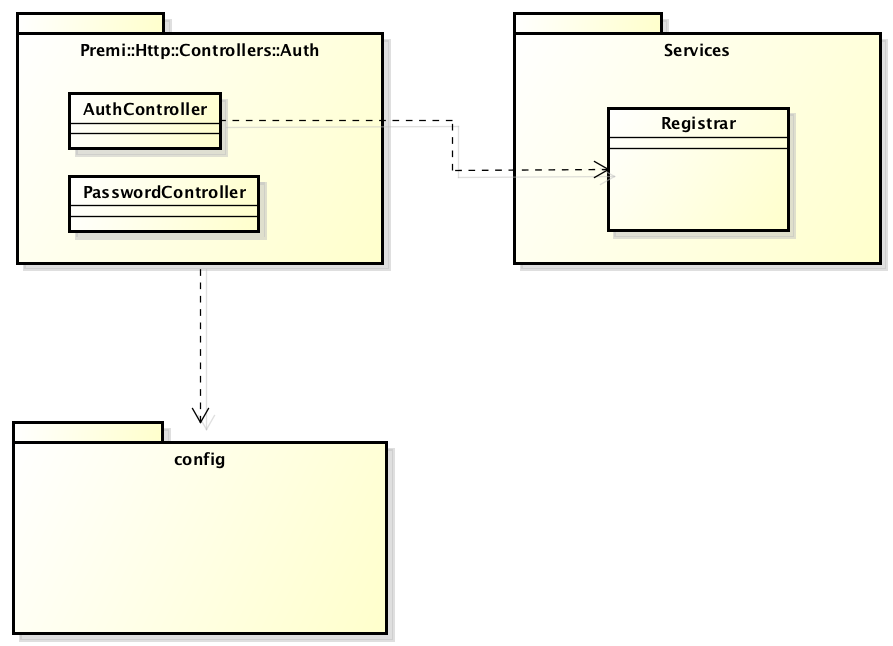
\includegraphics[width=0.9\linewidth]{img/premi_http_controllers_auth}
			\caption[Premi::Http::Controllers::Auth]{Premi::Http::Controllers::Auth}
			\label{fig:premi_http_controllers_auth}
		\end{figure}
	Laravel utilizza un semplice meccanismo di autenticazione. I file di configurazioni già documentate si trovano all'interno del package \textbf{config} che servono a ottimizzare il comportamento del servizio di autenticazione.		
	\subsubsection*{Classi contenute}
		\begin{itemize}
			\item Premi::Http::Auth::AuthController:
				\begin{itemize}
					\item \textbf{Descrizione}: AuthController gestisce le registrazioni di nuovi utenti e i loro accessi.
				\end{itemize}
			\item Premi::Http::Auth::PasswordController:
				\begin{itemize}
					\item \textbf{Descrizione:} PasswordController contiene la logica di aiuto agli utenti per la procedura di reset della password.
				\end{itemize}
		\end{itemize}
	Ognuno di questi controller usa un \gls{trait} che include i metodi necessari al loro corretto funzionamento.\\
	Per modificare i campi del form necessari alla registrazione di un nuovo utente, è sufficente modificare la classe Services::Registrar. Questa classe è responsabile della creazione e validazione dei nuovi utenti. Il metodo \textit{validator} di Registrar contiene le regole di validazione per i nuovi utenti, mentre il metodo \textit{create} di Registrar è responsabile della creazione di un nuovo record User nel database. Registrar è chiamato da AuthController tramite dei metodi contenuti nel \gls{trait} AuthenticatesAndRegistersUsers.
			
	\subsubsection*{Premi::Http::Controllers::ProjectController}
			\begin{itemize}
				\item \textbf{Descrizione}: Classe responsabile delle operazioni e della logica riguardante la gestione e la modifica di un progetto;
			\end{itemize}
			
   \subsubsection*{Premi::Http::Controllers::PresentationController}
			\begin{itemize}
				\item \textbf{Descrizione}: Classe responsabile delle operazioni e della logica riguardante la gestione e la modifica di una presentazione;
			\end{itemize}
			
	\subsubsection*{Premi::Http::Controllers::InfographicsController}
			\begin{itemize}
				\item \textbf{Descrizione}: Classe responsabile delle operazioni e della logica riguardante la gestione e la modifica di un'\gls{infografica};
			\end{itemize}
			
	\subsubsection*{Premi::Http::Controllers::SlideController}
			\begin{itemize}
				\item \textbf{Descrizione}: Classe responsabile delle operazioni e della logica riguardante la gestione e la modifica di una \gls{slide};
			\end{itemize}
		
\newpage
\subsection{Premi::Http::Middleware}
\begin{figure}[h]
\centering
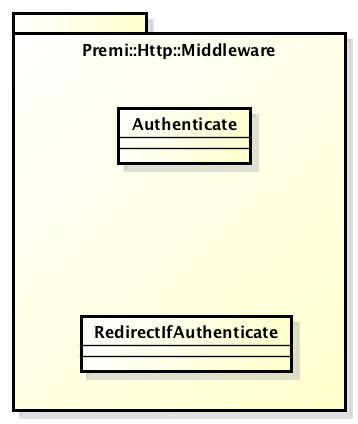
\includegraphics[width=0.7\linewidth]{img/premi_http_middleware}
\caption[Premi::Http::Middleware]{Premi::Http::Middleware}
\label{fig:premi_http_middleware}
\end{figure}

	\subsubsection*{Informazioni sul package}
	I middleware forniscono un meccanismo molto conveniente di filtraggio delle richieste HTTP in entrata.
	\subsubsection*{Classi contenute}
		\begin{itemize}
			\item \textbf{Premi::Http::Middleware::Autheticate:} verifica se l'utente dell'applicazione ha effettuato l'accesso correttamente;
			\item \textbf{Premi::Http::Middleware::RedirectIfAutheticate:} al verificarsi di un esito negativo del controllo precedente, il middleware effettua un redirect verso la schermata di login. In caso contrario, invece, tutto prosegue normalmente.
		\end{itemize}
\newpage
\subsection{Premi::Http::Request}
\begin{figure}[h]
\centering
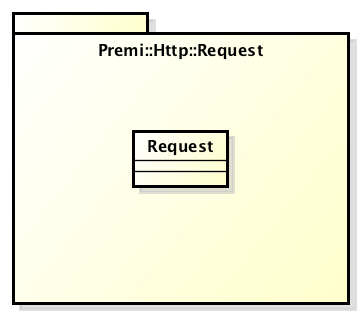
\includegraphics[width=0.7\linewidth]{img/premi_http_request}
\caption[Premi::Http::Request]{Premi::Http::Request}
\label{fig:premi_http_request}
\end{figure}
	\subsubsection*{Informazione sul package}
	La classe Facade Request garantisce l'accesso alla richiesta corrente contenuta nel container.

	
%\subsection{Premi::Back-End::Logic-Tier::Controller::ComponentController}
%	\subsubsection*{Informazioni sul package}
%		\begin{figure}[h]
%			\centering
%			\includegraphics[width=0.9\linewidth]{img/back-end_logic-tier_controller_componentcontroller}
%			\caption[Premi::Back-End::Logic-Tier::Controller::ComponentController]{Premi::Back-End::Logic-Tier::Controller::ComponentController}
%		\end{figure}
%		Il package contiene le classi dei controller per la gestione degli elementi di una \gls{slide}.
%		
%	\subsubsection*{Classi contenute}
%	\begin{itemize}
%		\item Premi::Back-End::Logic-Tier::Controller::ComponentController::ComponentController:
%		\begin{itemize}
%			\item \textbf{Descrizione}: classe che gestisce le operazioni e la logica applicativa di tutti i componenti della \gls{slide};
%			\item \textbf{Relazioni con altre classi}:
%			\begin{itemize}
%				\item Premi::Back-End::Logic-Tier::Controller::FrontController.
%			\end{itemize}
%		\end{itemize}
%		
%		\item Premi::Back-End::Logic-Tier::Controller::ComponentController::RealTimeDataController:
%		\begin{itemize}
%			\item \textbf{Descrizione}: classe che gestisce le operazioni e la logica applicativa dei componenti per i dati real-time della \gls{slide};
%			\item \textbf{Relazioni con altre classi}:
%			\begin{itemize}
%				\item Premi::Back-End::Logic-Tier::Controller::ComponentController::ComponentController.
%			\end{itemize}
%		\end{itemize}
%		
%		\item Premi::Back-End::Logic-Tier::Controller::ComponentController::ChartController:
%		\begin{itemize}
%			\item \textbf{Descrizione}: classe che gestisce le operazioni e la logica applicativa dei componenti per i grafici della \gls{slide};
%			\item \textbf{Relazioni con altre classi}:
%			\begin{itemize}
%				\item Premi::Back-End::Logic-Tier::Controller::ComponentController::ComponentController.
%			\end{itemize}
%		\end{itemize}
%		
%		\item Premi::Back-End::Logic-Tier::Controller::ComponentController::ImageController:
%		\begin{itemize}
%			\item \textbf{Descrizione}: classe che gestisce le operazioni e la logica applicativa dei componenti per le immagini della \gls{slide};
%			\item \textbf{Relazioni con altre classi}:
%			\begin{itemize}
%				\item Premi::Back-End::Logic-Tier::Controller::ComponentController::ComponentController.
%			\end{itemize}
%		\end{itemize}
%		
%		\item Premi::Back-End::Logic-Tier::Controller::ComponentController::TableController:
%		\begin{itemize}
%			\item \textbf{Descrizione}: classe che gestisce le operazioni e la logica applicativa dei componenti per le tabelle della \gls{slide};
%			\item \textbf{Relazioni con altre classi}:
%			\begin{itemize}
%				\item Premi::Back-End::Logic-Tier::Controller::ComponentController::ComponentController.
%			\end{itemize}
%		\end{itemize}
%		
%		\item Premi::Back-End::Logic-Tier::Controller::ComponentController::TextController:
%		\begin{itemize}
%			\item \textbf{Descrizione}: classe che gestisce le operazioni e la logica applicativa dei componenti per le caselle di testo della \gls{slide};
%			\item \textbf{Relazioni con altre classi}:
%			\begin{itemize}
%				\item Premi::Back-End::Logic-Tier::Controller::ComponentController::ComponentController.
%			\end{itemize}
%		\end{itemize}
%	\end{itemize}
%	

\newpage
\subsection{Premi::Model}
	\subsubsection*{Informazioni sul package}
\begin{figure}[h]
\centering
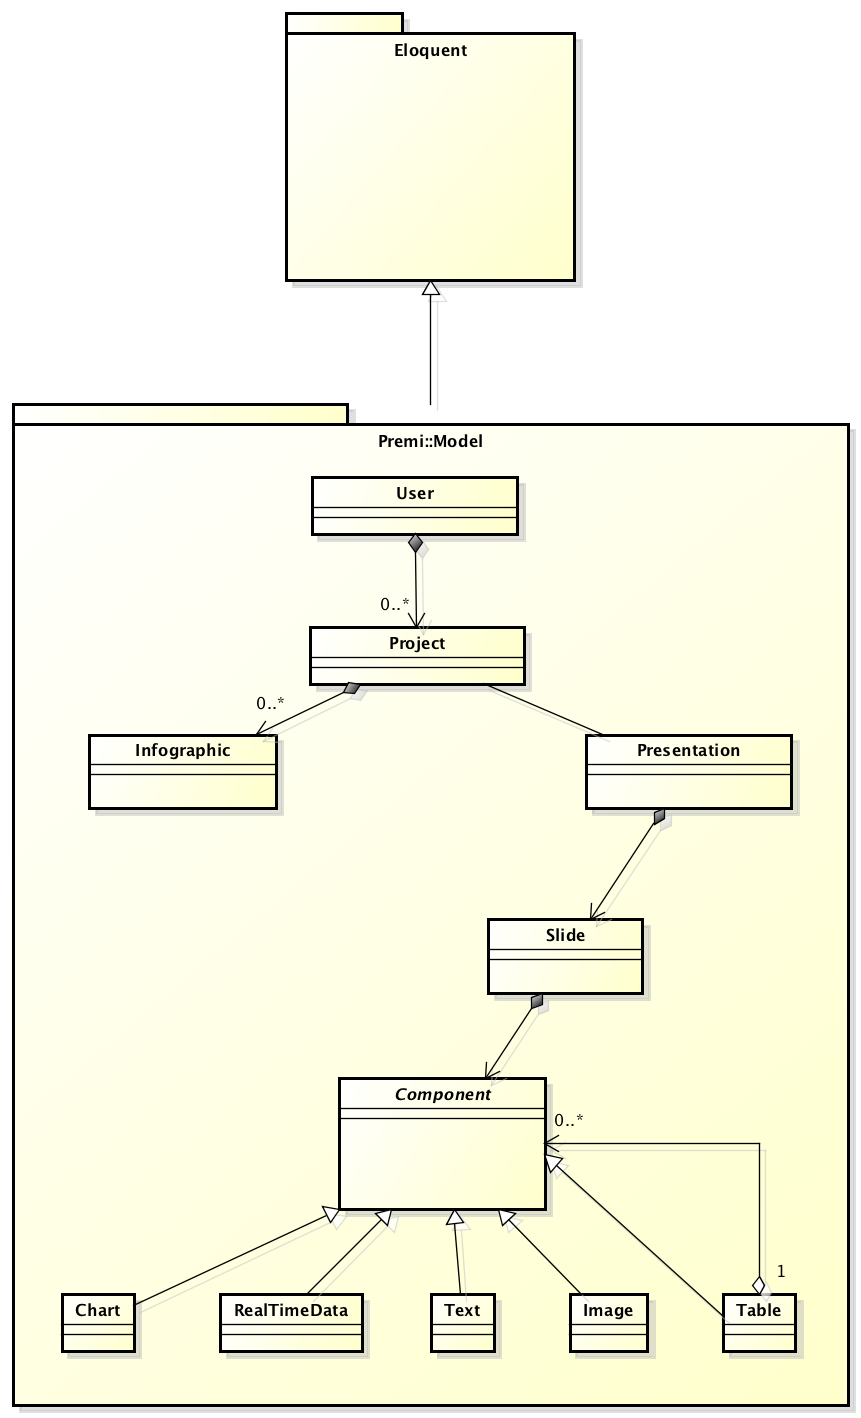
\includegraphics[width=0.7\linewidth]{img/premi_http_model}
\caption[Premi::Model]{Premi::Model}
\label{fig:premi_http_model}
\end{figure}
		Il package contiene la struttura delle classi di tutti i componenti dell'applicazione.
	
	\subsubsection*{Classi contenute}
	\begin{itemize}
		\item Premi::Model::User:
		\begin{itemize}
			\item \textbf{Descrizione:} classe contenente le informazioni di un utente.
		\end{itemize}
		\item Premi::Model::Project:
		\begin{itemize}
			\item \textbf{Descrizione}: classe base contenente le informazioni principali di un progetto.
		\end{itemize}
			
		\item Premi::Model::Infographic:
		\begin{itemize}
			\item \textbf{Descrizione:} classe che rappresenta le infografiche associate a un progetto;
			\item \textbf{Relazione con altre classi}:
			\begin{itemize}
				\item Premi::Model::Project.
			\end{itemize}
		\end{itemize}
		
		\item Premi::Model::Presentation:
		\begin{itemize}
			\item \textbf{Descrizione:} classe che rappresenta la presentazione del progetto;
			\item \textbf{Relazione con altre classi}:
			\begin{itemize}
				\item Premi::Model::Project.
			\end{itemize}
		\end{itemize}
		
		\item Premi::Model::Slide:
		\begin{itemize}
			\item \textbf{Descrizione:} classe che rappresenta le \gls{slide} che compongono una presentazione;
			\item \textbf{Relazione con altre classi}:
			\begin{itemize}
				\item Premi::Model::Project.
			\end{itemize}
		\end{itemize}
		
		\item Premi::Model::Component:
		\begin{itemize}
			\item \textbf{Descrizione:} classe base che rappresenta i componenti di cui è formata una \gls{slide};
			\item \textbf{Relazione con altre classi}:
			\begin{itemize}
				\item Premi::Model::Project.
			\end{itemize}
		\end{itemize}
		
		\item Premi::Model::Chart:
		\begin{itemize}
			\item \textbf{Descrizione:} classe che rappresenta l'elemento "grafico" che può essere inserito in una \gls{slide};
			\item \textbf{Relazione con altre classi}:
			\begin{itemize}
				\item Premi::Model::Project.
			\end{itemize}
		\end{itemize}
		
		\item Premi::Model::RealTimeData:
		\begin{itemize}
			\item \textbf{Descrizione:} classe che rappresenta l'elemento "dati real-time" che può essere inserito in una \gls{slide};
			\item \textbf{Relazione con altre classi}:
			\begin{itemize}
				\item Premi::Model::Project.
			\end{itemize}
		\end{itemize}
		
		\item Premi::Model::Text:
		\begin{itemize}
			\item \textbf{Descrizione:} classe che rappresenta l'elemento "testo" che può essere inserito in una \gls{slide};
			\item \textbf{Relazione con altre classi}:
			\begin{itemize}
				\item Premi::Model::Project.
			\end{itemize}
		\end{itemize}
		
		\item Premi::Model::Image:
		\begin{itemize}
			\item \textbf{Descrizione:} classe che rappresenta l'elemento "immagine" che può essere inserito in una \gls{slide};
			\item \textbf{Relazione con altre classi}:
			\begin{itemize}
				\item Premi::Model::Project.
			\end{itemize}
		\end{itemize}
		
		\item Premi::Model::Table:
		\begin{itemize}
			\item \textbf{Descrizione:} classe che rappresenta l'elemento "tabella" che può essere inserito in una \gls{slide};
			\item \textbf{Relazione con altre classi}:
			\begin{itemize}
				\item Premi::Model::Project.
			\end{itemize}
		\end{itemize}
	\end{itemize}
	
\subsubsection*{Informazioni su Eloquent}
Eloquent è l'ORM(Object Relational Mapping) incluso in Laravel: un'implementazione di Active Record. Tutti i model estendono  Eloquent in modo da creare e gestire l'interazione con la collection.

\subsection{Data-Tier}
\begin{figure}[h]
\centering
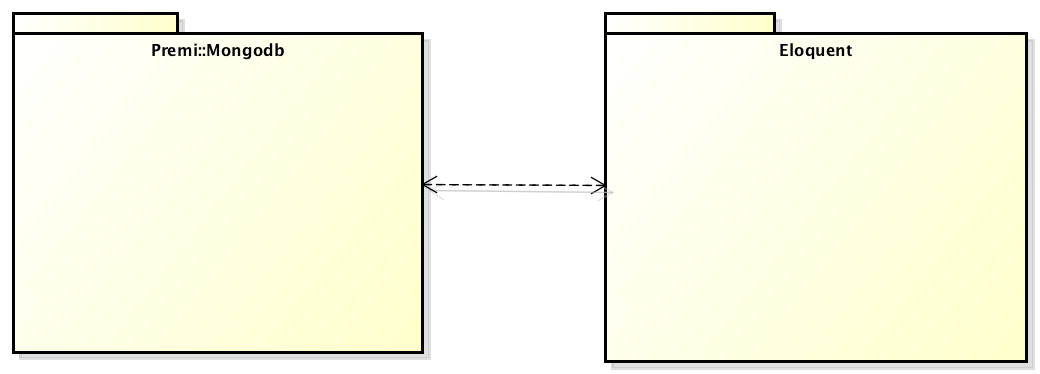
\includegraphics[width=0.7\linewidth]{img/premi_mongodb}
\caption[Premi::Mongodb]{Premi::Mongodb}
\label{fig:premi_mongodb}
\end{figure}
\subsubsection*{Informazioni sul package}
Ogni collection nel database trova una sua corrispondenza in un Model, il quale ha proprio il compito di gestire l'interazione con la collection stessa. Una volta definito il model si è pronti a selezionare un record, crearne di nuovi ed in generale lavorare con la collection. La sintassi è molto semplice: Laravel mette a disposizione le query tramite il Model Eloquent.

\newpage

\subsection{Scenari}
	\subsubsection{Gestione richiesta di registrazione}
	Il seguente diagramma rappresenta lo scenario con il quale viene gestita una richiesta di registrazione. La richiesta parte da signupService() e viene gestita da \textit{AuthController} che controlla il corretto inserimento dei dati e invia il responso a \textit{AuthController}, tramite postRegister(). Viene poi ritornata create() che indica a signupService che l'utente è stato creato.
	\begin{figure}[H]
		\centering
		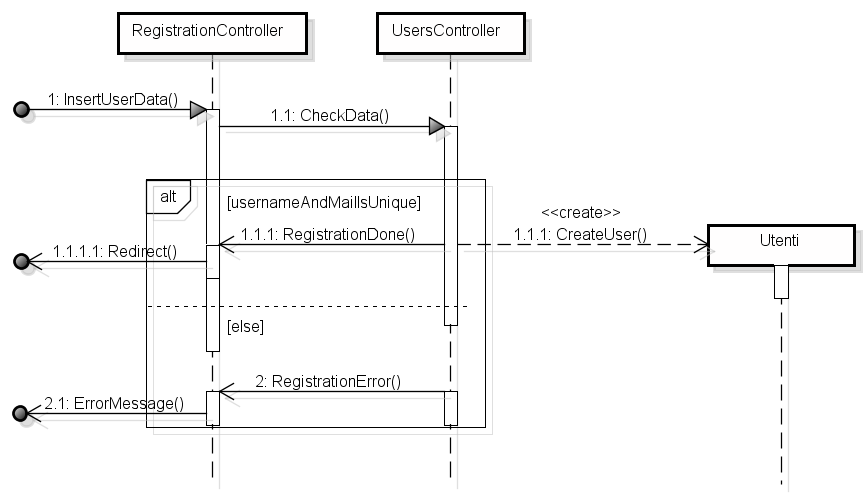
\includegraphics[scale=0.5]{img/register.png}
		\caption{Diagrammi di sequenza - Richiesta di registrazione}
	\end{figure}

\newpage
	\subsubsection{Gestione richiesta di autenticazione}
	Il loginService() invia una richiesta che viene gestita da \textit{AuthController}, il quale invia una postLogin() a \textit{AuthenticatesUsers}. Qui li scenari possibili sono due: nel primo caso la procedura va a buon fine e \textit{AuthenticatesUsers} emette un response() verso \textit{AuthController} che segnala a loginService() tramite una redirect() che l'autenticazione ha avuto successo. Nel secondo caso \textit{AuthenticatesUsers} invia una getFailedLoginMessage() a \textit{AuthController} che segnala l'errore a loginService() tramite un failed();

	\begin{figure}[H]
		\centering
		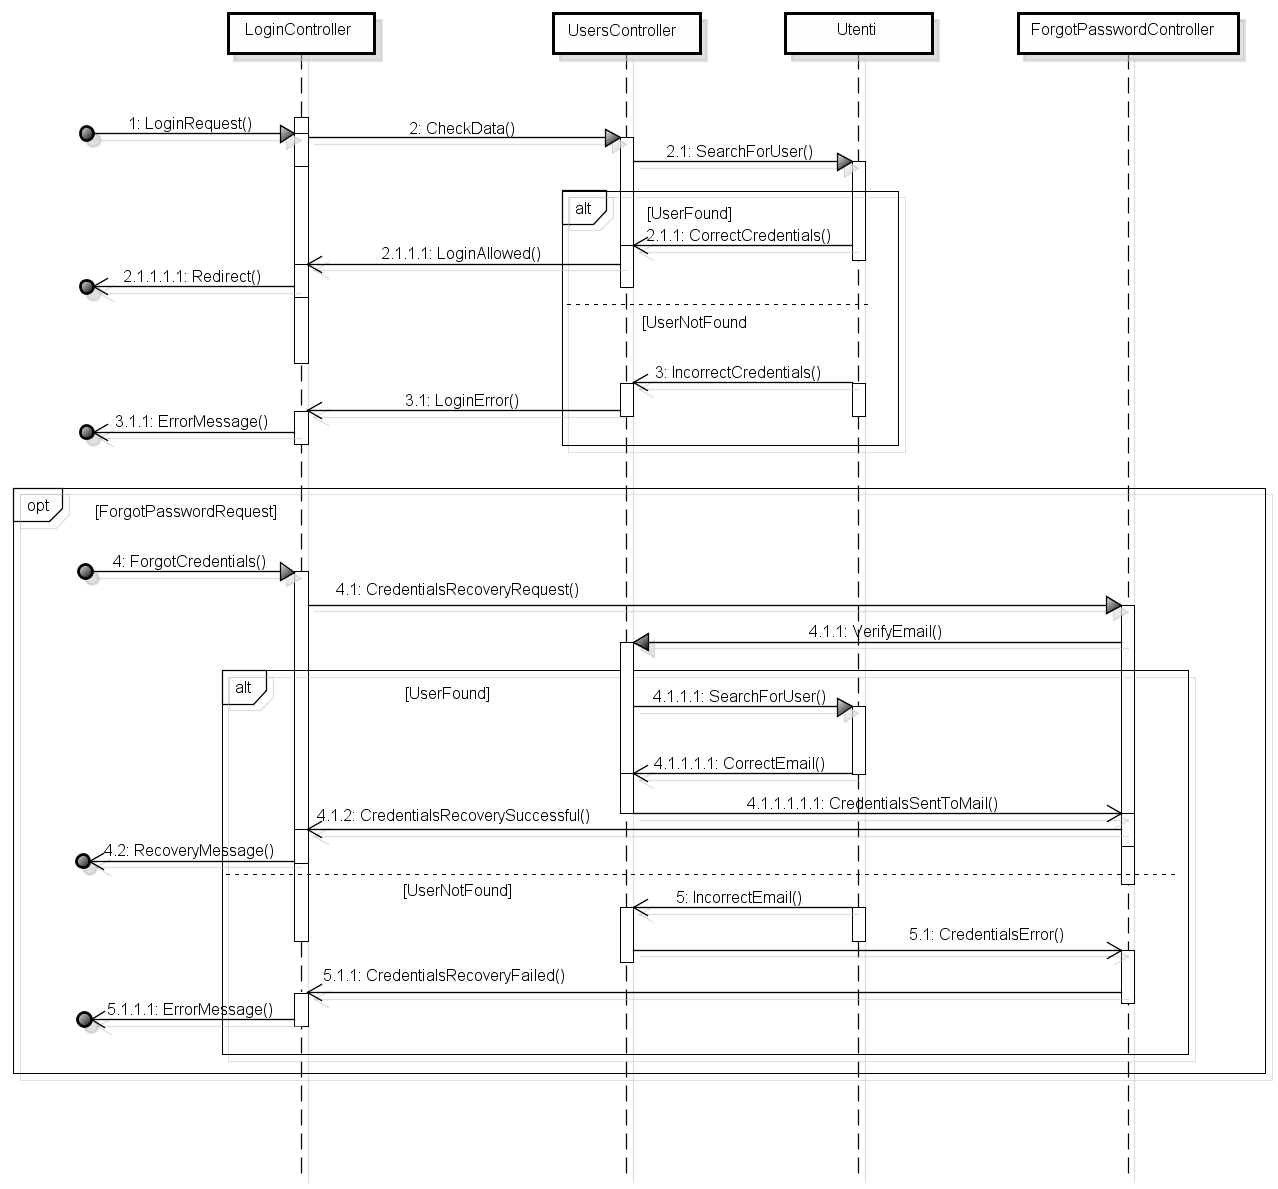
\includegraphics[width=0.9\textwidth]{img/login.png}
		\caption{Diagrammi di sequenza - Richiesta di autenticazione}
	\end{figure}

\newpage
	\subsubsection{Gestione richiesta di ricerca di un progetto}
	Una richiesta di ricerca inoltrata da searchService() viene gestita da \textit{SearchCtrl} che invia una search() a \textit{SearchController}. A questo punto viene ritornato un showResults a \textit{SearchCrtl} che a sua volta segnala i risultati ottenuti a searchService() con un sendResults().
	\begin{figure}[H]
		\centering
		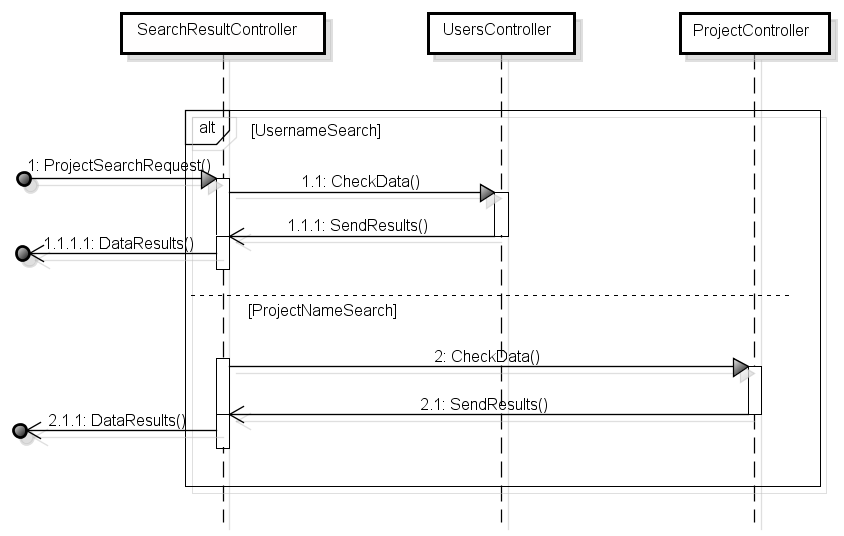
\includegraphics[scale=0.5]{img/search.png}
		\caption{Diagrammi di sequenza - Richiesta di ricerca di un progetto}
	\end{figure}
	
\newpage	
	\subsubsection{Gestione richiesta di visualizzazione di una presentazione}
	presentationService() invia una richiesta gestita da \textit{PresentationCtrl}. Esso invia una loadSlides() a \textit{PresentationController} il quale elabora le informazioni e emette una show() indirizzata a \textit{PresentationCtrl}. Questo controller alla fine invia il risultato di ritorno a presentationService() tramite il metodo slide in (slidesSVG).
	
	\begin{figure}[H]
		\centering
		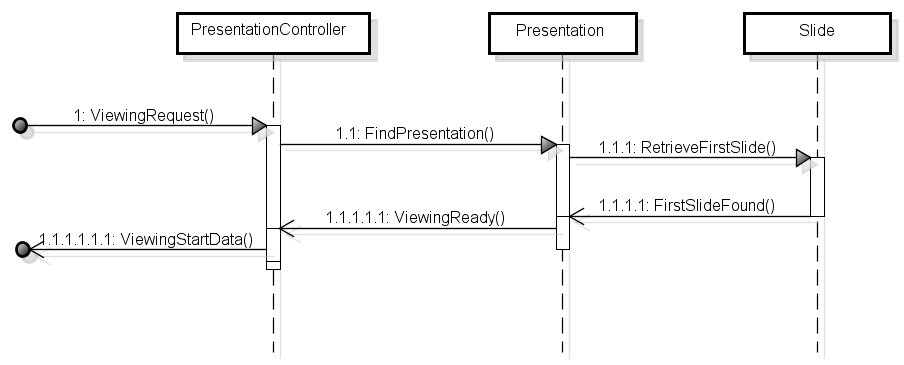
\includegraphics[scale=0.5]{img/view.png}
		\caption{Diagrammi di sequenza - Richiesta di visualizzazione di una presentazione}
	\end{figure} 
	
	
	\subsubsection{Gestione richiesta di creazione di un progetto}
	presentationEditorService() invia una richiesta che viene presa in carico dal \textit{PresentationCtrl}, che invia una createPresentation() a \textit{PresentationController}. Quest'ultimo elabora i dati ricevuti ed invia una show() a \textit{PresentationCtrl} che restituisce il risultato a presentationService() tramite il metodo slide in (slidesSVG).
	
	\begin{figure}[H]
		\centering
		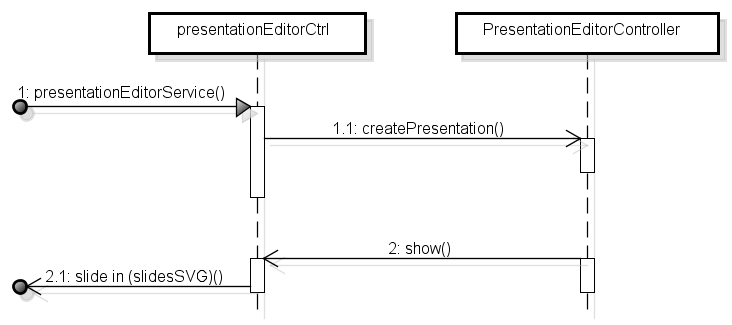
\includegraphics[scale=0.5]{img/create.png}
		\caption{Diagrammi di sequenza - Richiesta di creazione di un progetto}
	\end{figure}
	
\newpage	
	\subsubsection{Gestione richiesta di apertura di un progetto}
	Viene inviata una richiesta di apertura di un progetto da parte di openProjectService() e gestita da \textit{myProjectCtrl}. Questo invia una openProject() a \textit{Project} il quale invia load() gestita sempre da \textit{myProject}. Infine a openProjectService() viene passato il risultato delle operazioni effettuate tramite showProjectService().
	
	\begin{figure}[H]
		\centering
		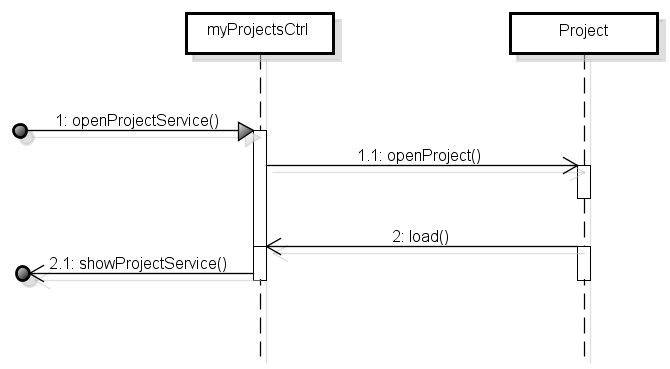
\includegraphics[scale=0.5]{img/open.png}
		\caption{Diagrammi di sequenza - Richiesta di apertura di un progetto}
	\end{figure}
	
	\newpage
	
	\subsubsection{Gestione richiesta di modifica di un progetto}
	slideEditorService() invia una richiesta gestita da \textit{SlideEditorCtrl}, che invia a sua volta un slideEditor() gestito da \textit{SlideController}. Esso invia una showEditor() a \textit{SlideEditorCtrl} che risponde con slideEditorShowService() alla chiamata iniziale.
	
	\begin{figure}[H]
		\centering
		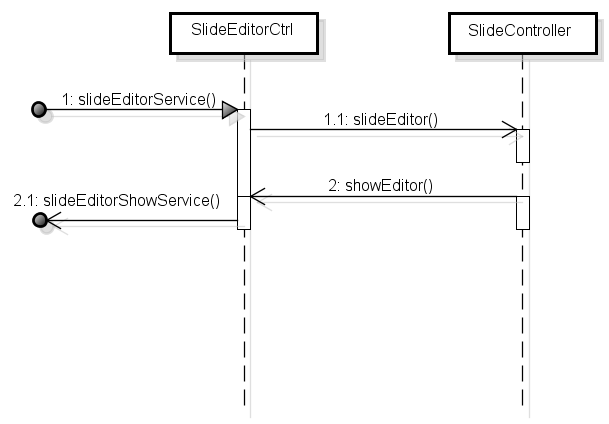
\includegraphics[scale=0.5]{img/modify.png}
		\caption{Diagrammi di sequenza - Richiesta di modifica di un progetto}
	\end{figure}
	
	
	
	\subsubsection{Gestione richiesta salvataggio di un progetto}
	saveProjectService() invia una richiesta che viene gestita da \textit{myProjectCtrl}, questo invia una saveProject() a \textit{ProjectController} che elabora i dati ed emette una store(). store() viene gestita da \textit{myProjectCtrl} che risponde alla chiamata iniziale tramite saveProjectService().
	
	\begin{figure}[H]
		\centering
		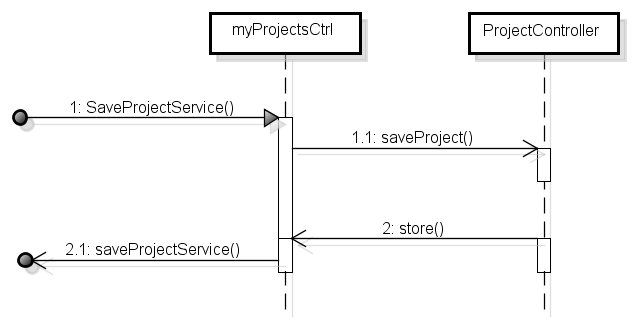
\includegraphics[scale=0.5]{img/save.png}
		\caption{Diagrammi di sequenza - Richiesta di salvataggio di un progetto}
	\end{figure}
	\newpage


\newpage

\section{Design Pattern}\label{pattern}
I \gls{Design Pattern} sono un modello da applicare per la risoluzione di problemi ricorrenti. Essi possono essere organizzati in quattro categorie:
\begin{itemize}
	\item \textbf{Architetturali}: dividono il sistema in sottosistemi specificandone le responsabilità e dettando linee guida per organizzare le relazioni tra loro;
	\item \textbf{Creazionali}: forniscono un'astrazione del processo d'istanziazione degli oggetti. Aiutano a rendere il sistema indipendente dalle modalità d'istanziazione, composizione e rappresentazione degli oggetti utilizzati;
	\item \textbf{Strutturali}: si occupano della composizione di classi ed oggetti per formare Strutture complesse;
	\item \textbf{Comportamentali}: si occupano della gestione degli algoritmi e delle responsabilità di oggetti che collaborano tra loro.
\end{itemize}

\subsection{Pattern Architetturali}
\begin{itemize}
	\item Model-View-Controller(\gls{MVC})
	\begin{itemize}
		\item \textbf{Descrizione:} prevede la separazione in tre componenti:
		\begin{itemize}
			\item \textit{model}: fornisce i metodi per accedere ai dati utili all'applicazione;
			\item \textit{view}:  visualizza i dati contenuti nel model e si occupa delle interazione esterne;
			\item \textit{controller}: esegue funzionalità chiamate dalle view e modifica lo stato di model e/o view.
		\end{itemize}
		\item \textbf{Contesto d'utilizzo:} \gls{Front-End} \newline È stato adottato perché permette di organizzare modularmente gli strati software mantenendo una struttura che permette di lavorare agevolmente con il \gls{framework} \gls{Angular}.js. Per l'utilizzo di questo framework è stata applicata una variazione al pattern in modo da inserire anche le componenti per le direttive e i servizi richiesti.
		\begin{figure}[h]
			\centering
			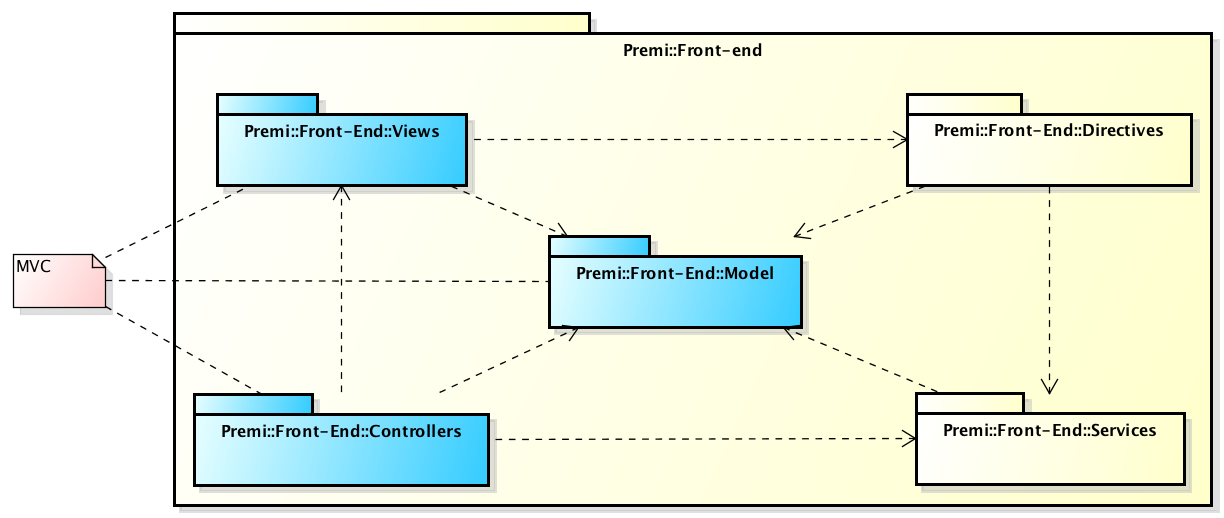
\includegraphics[width=\linewidth]{img/front-end_mvc}
			\caption[MVC Pattern - Premi::Front-End]{MVC Pattern - Premi::Front-End}
		\end{figure}
	\end{itemize}
\end{itemize}

\subsection{Pattern Strutturali}
\begin{itemize}
	\item Composite
	\begin{itemize}
		\item \textbf{Descrizione:} permette di comporre oggetti in strutture ad albero per rappresentare gerarchie in grado di trattare componenti foglia oppure composti allo stesso modo.
		\item \textbf{Contesto d'utilizzo:} Premi::Front-End::Model. È stato adottato nei model del \gls{Front-End} per creare la struttura di un componente della slide. 
		\begin{figure}[h]
			\centering
			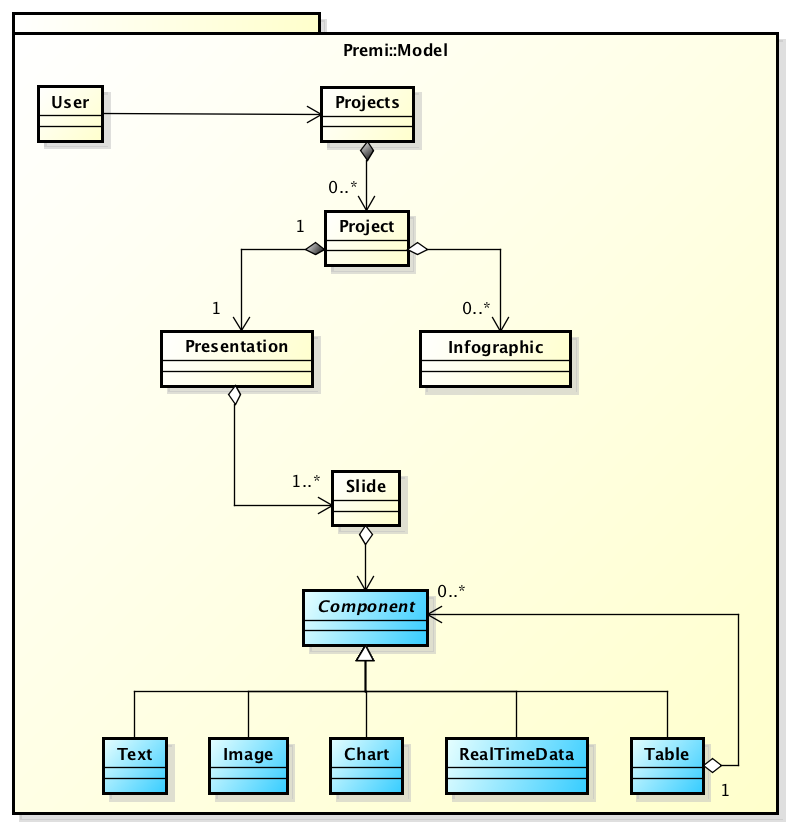
\includegraphics[width=0.5\linewidth]{img/front-end_model_composite}
			\caption[Composite Pattern - Premi::Front-End::Model]{Composite Pattern - Premi::Front-End::Model}
		\end{figure}
	\end{itemize}

\end{itemize}

\subsection{Pattern Comportamentali}
\begin{itemize}
	\item Command
	\begin{itemize}
		\item \textbf{Descrizione:} permette di incapsulare una richiesta in un oggetto in modo da variare il risultato a seconda di un parametro.
		\item \textbf{Contesto d'utilizzo:} \gls{Front-End} e \gls{Back-End}. I casi sono principalmente i seguenti:
		\begin{itemize}
			\item \gls{Front-End}: nella modalità "edit" di una \gls{slide}, a seguito di un click su un componente;
			\item \gls{Front-End}: nella modalità "edit" oppure durante uno slideshow, nel momento in cui una \gls{slide} deve disegnare le sue componenti con un metodo della forma drawComponent(id,tipo);
			\item \gls{Back-End}: nel momento in cui devo salvare un componente (la classe Premi::\gls{Back-End}::Data-Tier::DataTierFrontController deve essere in grado di selezionare il mapper adeguato al tipo di dati).
		\end{itemize}
	\end{itemize}
\end{itemize}


Nel progetto sono stati adottati anche adottati i seguenti stili architetturali:
\begin{itemize}
	\item Three-Tier
	\begin{itemize}
		\item \textbf{Descrizione:} prevede la suddivisione dell'applicazione in tre diversi moduli o strati dedicati rispettivamente alla interfaccia utente, alla logica funzionale (\gls{business} logic) e alla gestione dei dati persistenti.
		\item \textbf{Contesto d'utilizzo:} \gls{Back-End}\newline È stato adottato perché permette di organizzare modularmente gli strati software secondo una logica che si presta molto bene alla realtà da modellare.
	\end{itemize}
	\begin{figure}[h]
		\centering
		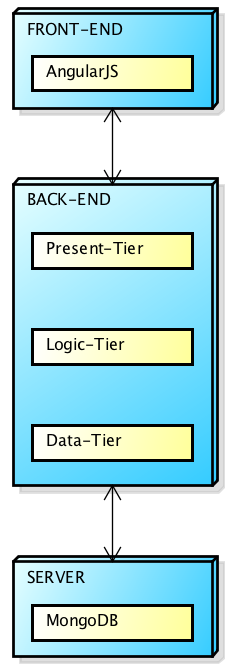
\includegraphics[width=0.2\linewidth]{img/architettura_generale_three}
		\caption[Three Tier - Premi]{Three Tier - Premi}
	\end{figure}
\end{itemize}
\newpage

\section{Diagrammi di attività}
Di seguito verranno presentati i diagrammi di attività che descrivono le iterazioni tra l'utente e il software \PROGETTO.
È stato disegnato un diagramma ad alto livello che descrive le attività principali, le quali verranno poi analizzate in dettaglio tramite dei sotto-diagrammi specifici. Per rendere la lettura del diagramma più semplice, é stato scelto di usare il nome in rosso per le attività che sono da considerarsi di alto livello, descritte poi più approfonditamente in sotto-attività tramite i relativi diagrammi. I riquadri con testo normale invece sono invece da intendersi come singole attività.

\subsection{Attività principali}
L'utente una volta avviato il programma ha la possibilità di \textit{Effettuare una ricerca}, \textit{Visualizzare un progetto}, \textit{Registrarsi}, \textit{Autenticarsi} e, una volta autenticato, di \textit{Creare un nuovo progetto}, \textit{Aprire un progetto}, \textit{Modificare un progetto} e \textit{Salvare un progetto}. Queste sono le principali attività dell'applicazione e possono essere utilizzate in parallelo senza che le singole attività vengano interrotte (figura 2).

\begin{figure}[p] 
	\centering 
	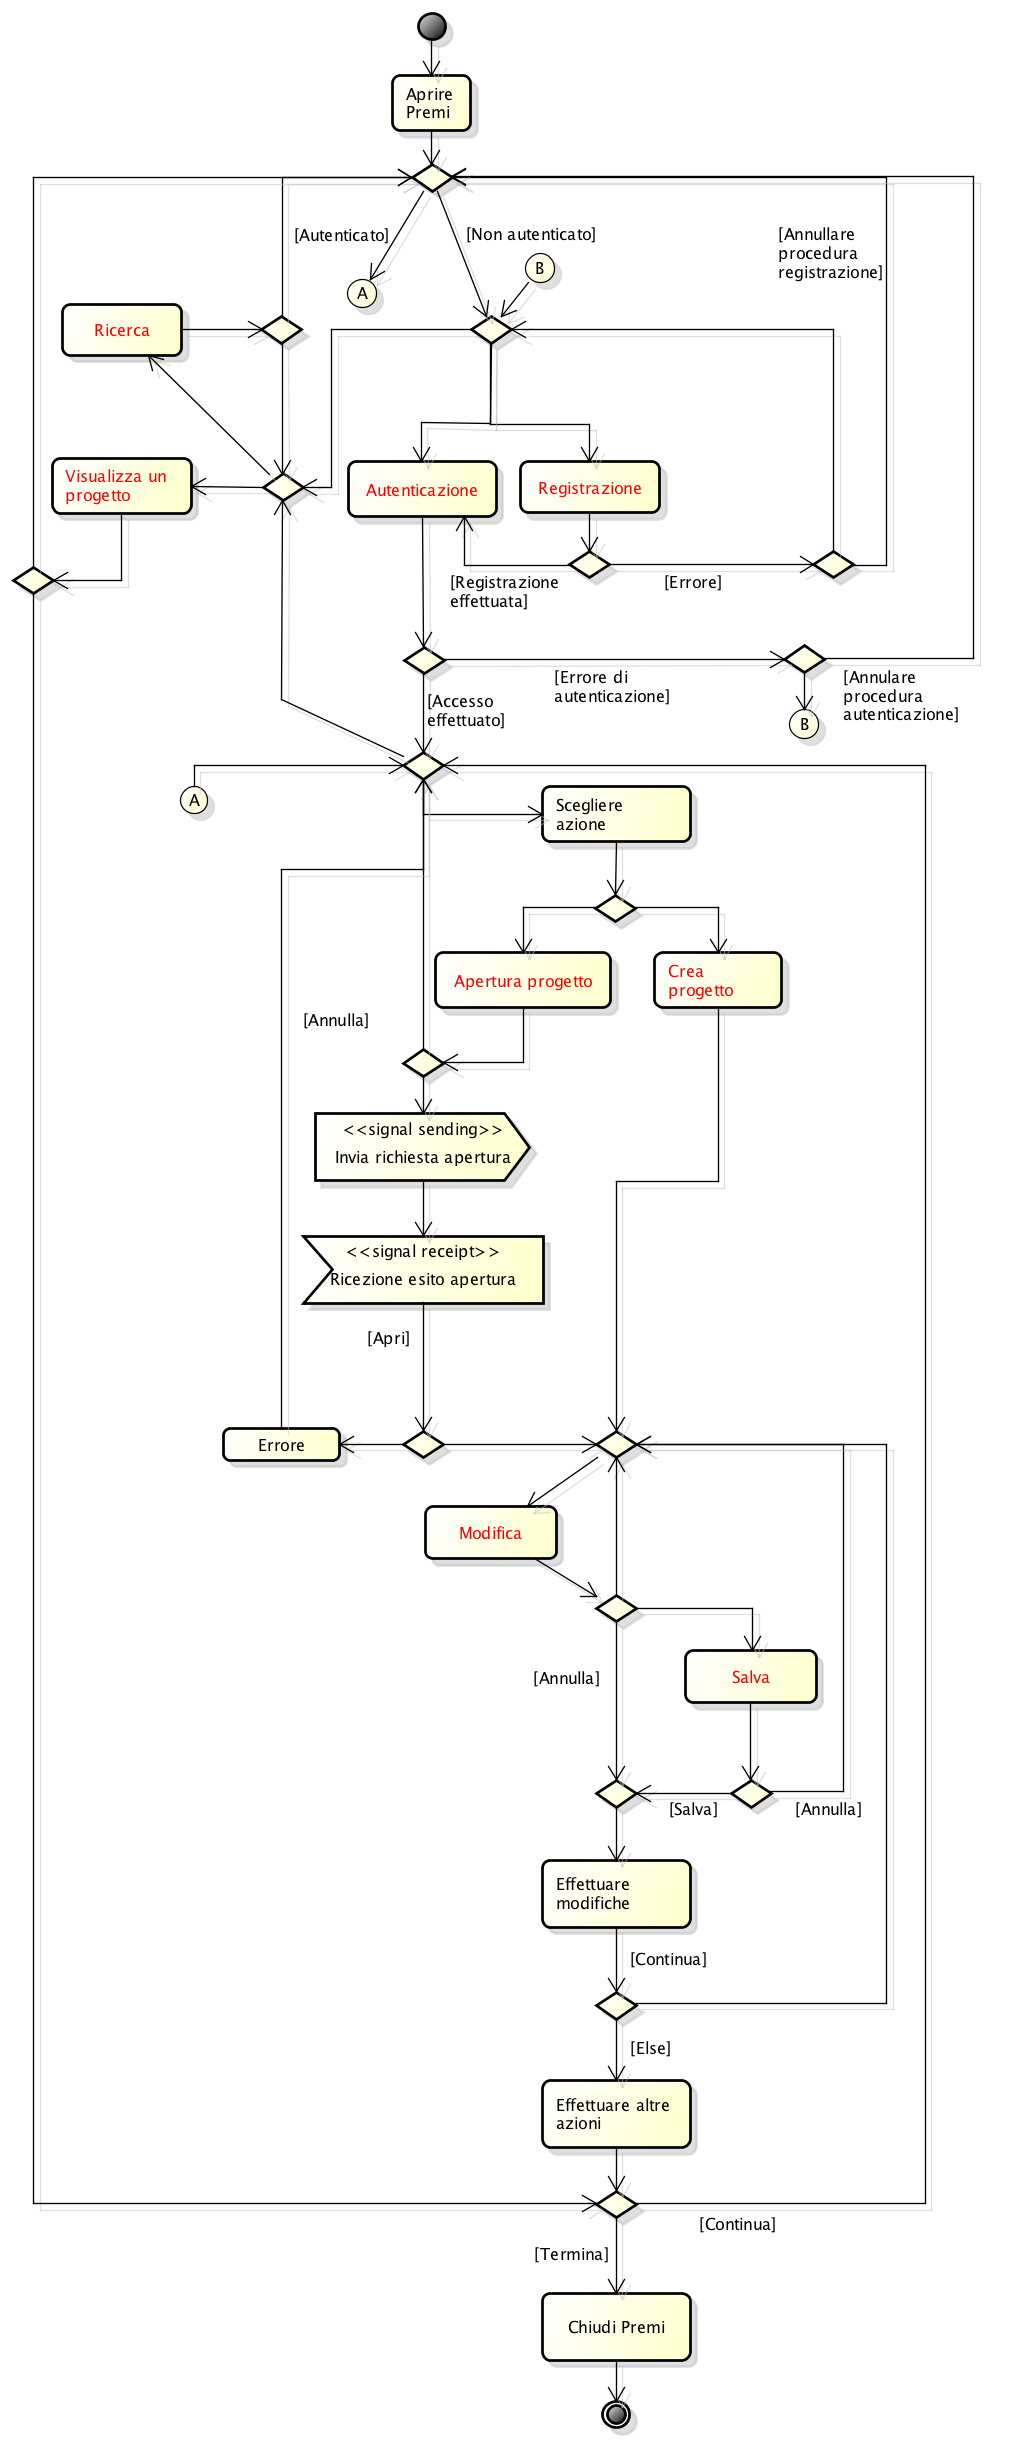
\includegraphics[height=20cm, keepaspectratio] {img/activity_diagram.png} 
	\caption{Diagramma attività - Attività principali dell'applicativo \PROGETTO} 
\end{figure}

\newpage

\subsection{Ricerca di un progetto}
\begin{figure}[h] 
	\centering 
	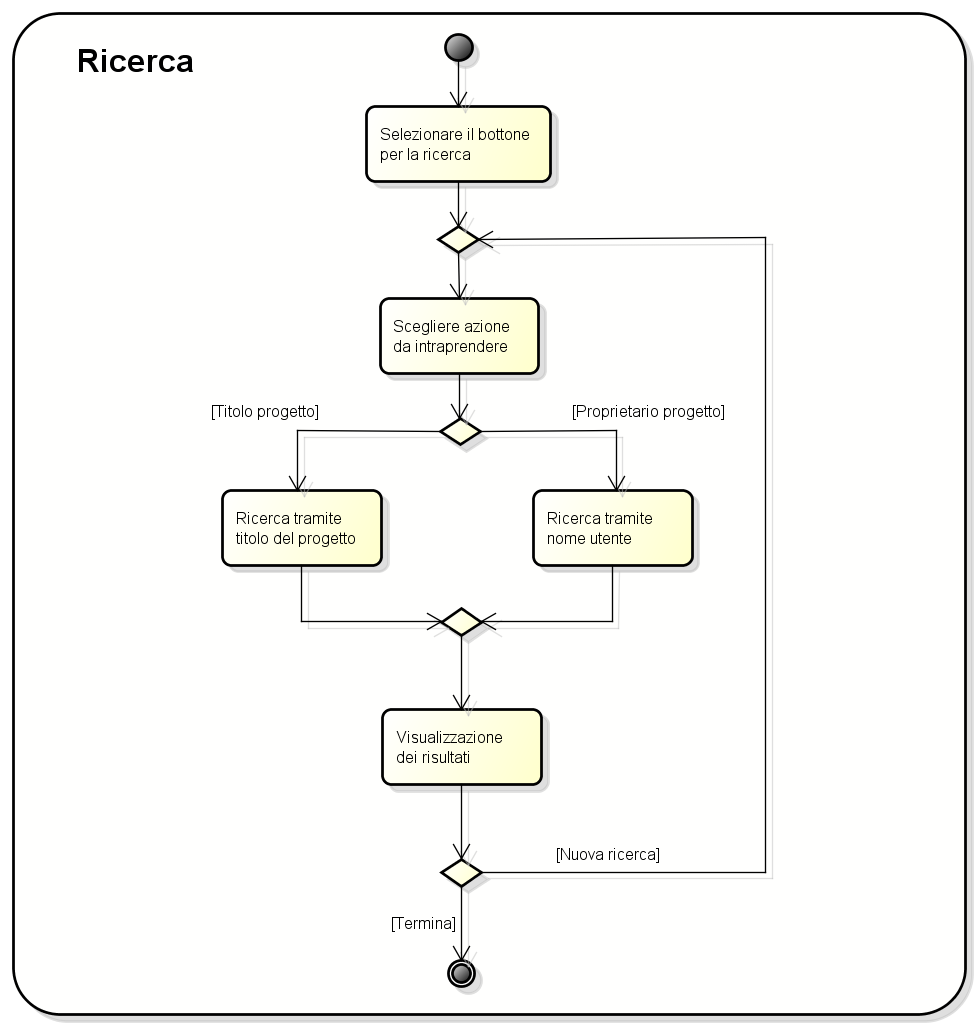
\includegraphics[scale=0.3] {img/activity_ricerca.png} 
	\caption{Diagramma attività - Ricerca di un progetto} 
\end{figure}
L'attività di ricerca di un progetto in figura 3 comprende le azioni di ricerca tramite titolo del progetto, ricerca tramite nome utente e visualizzazione dei risultati della ricerca. Una volta visualizzati i risultati, opzionalmente l'utente può effettuare un'altra ricerca.
\newpage

\subsection{Visualizzare un progetto}
\begin{figure}[h] 
	\centering 
	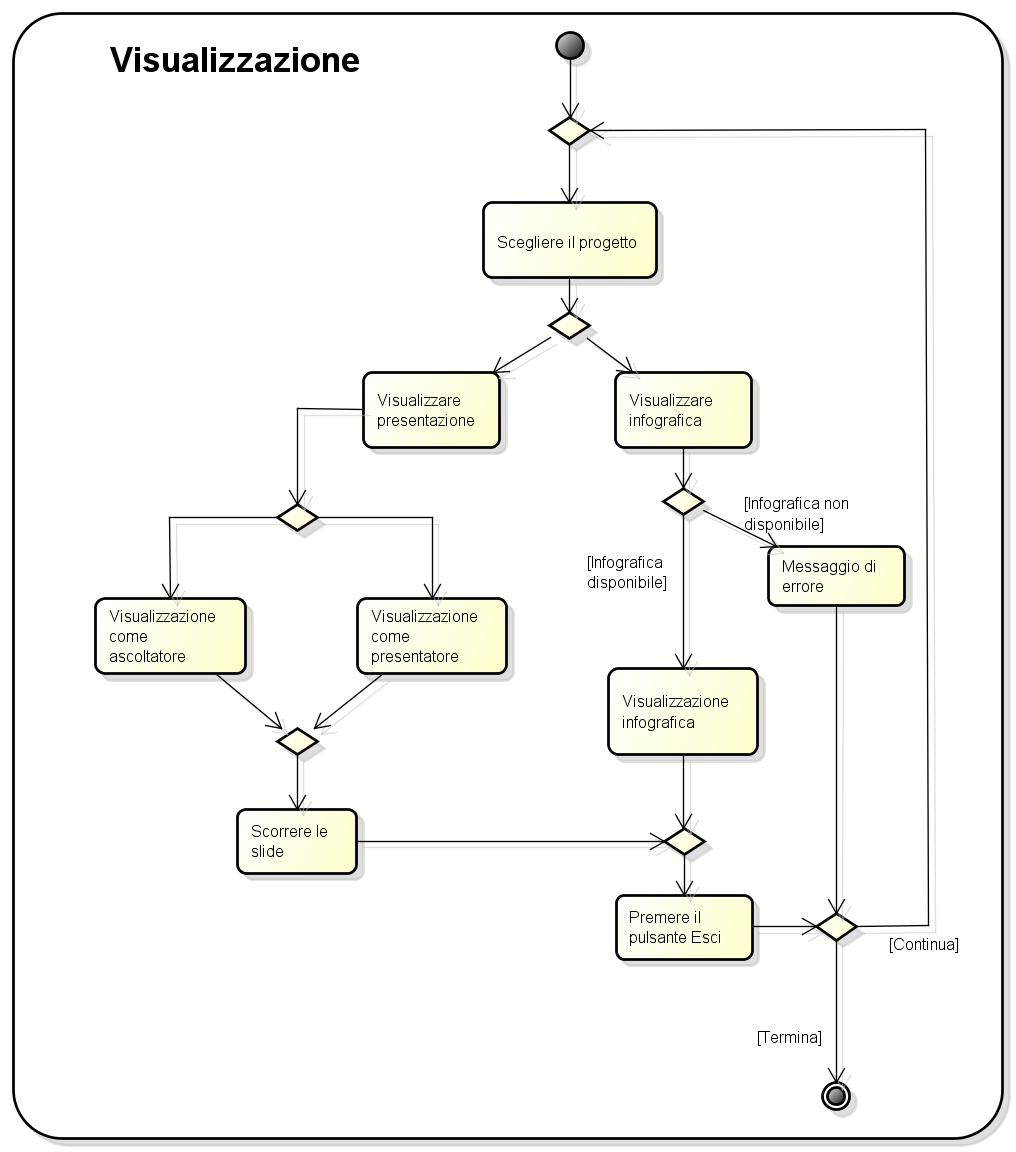
\includegraphics[scale=0.3] {img/activity_visualizza.png} 
	\caption{Diagramma attività - Visualizzare un progetto} 
\end{figure}
L'attività di visualizzazione di un progetto in figura 4 permette all'utente, una volta scelto il progetto, di visualizzare la presentazione oppure l'\gls{infografica} legata al progetto (se essa é disponibile). Nel caso si scelga di visualizzare una presentazione l'utente può scegliere se visualizzarla in modalità ascoltatore o presentatore, una volta fatta la decisione si può muovere tra le slide.
\newpage


\subsection{Registrazione}
\begin{figure}[h] 
	\centering 
	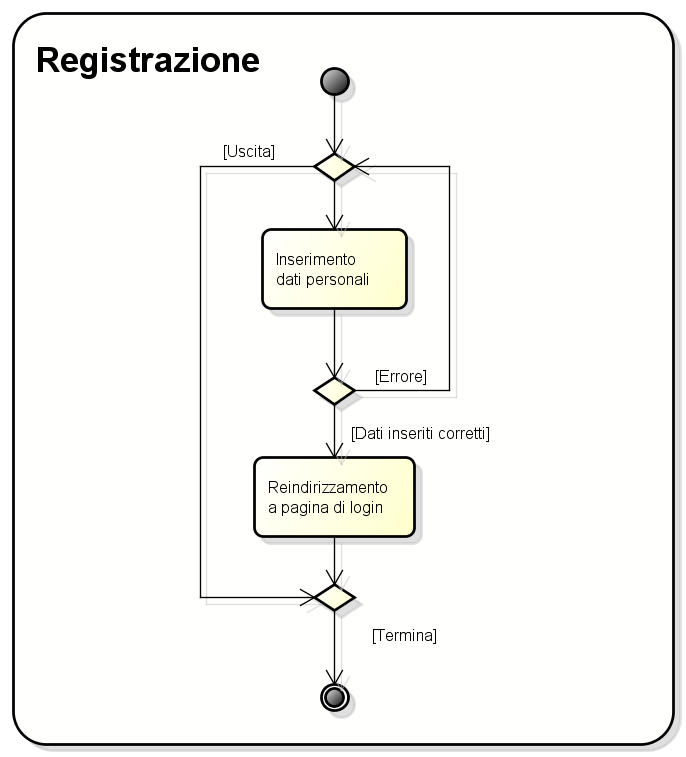
\includegraphics[scale=0.3] {img/activity_registrazione.png} 
	\caption{Diagramma attività - Registrazione} 
\end{figure}
La figura 5 rappresenta l'attività di registrazione di un utente. Una volta premuto il pulsante di registrazione, l'utente deve inserire i propri dati e può scegliere di annullare l'inserimento di un dato e reinserirlo senza dover ripetere la procedura. Una volta confermati i dati inseriti, se corretti l'utente viene registrato e reindirizzato alla pagina di login.
\newpage


\subsection{Autenticazione}
\begin{figure}[h] 
	\centering 
	\includegraphics[scale=0.3] {img/activity_autenticazione.png} 
	\caption{Diagramma attività - Autenticazione} 
\end{figure}
L'attività di autenticazione in figura 6 permette all'utente di inserire le proprie credenziali, di annullarne l'inserimento nel caso in cui si sbagli a digitarle e di confermarle. Nel caso in cui l'utente non ricordi più le proprie credenziali ha la possibilità di eseguire la procedura di recupero dei propri dati, alla fine della quale viene riportato alla pagina di login.
\newpage


\subsection{Creazione di un progetto}
\begin{figure}[h] 
	\centering 
	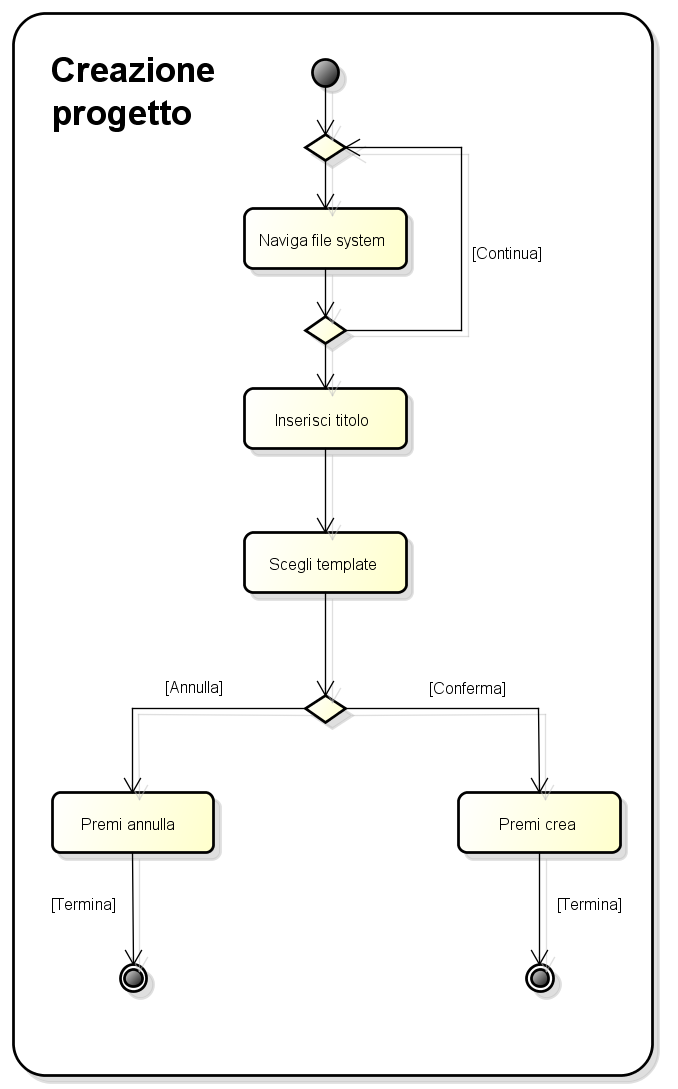
\includegraphics[scale=0.3] {img/activity_creazione.png} 
	\caption{Diagramma attività - Creazione di un progetto} 
\end{figure}
L'attività di creazione in figura 7 permette ad un utente autenticato di creare un nuovo progetto, di selezionare dove sarà salvato il progetto e richiede di inserire un titolo e di scegliere un template.
\newpage


\subsection{Apertura di un progetto}
\begin{figure}[h] 
	\centering 
	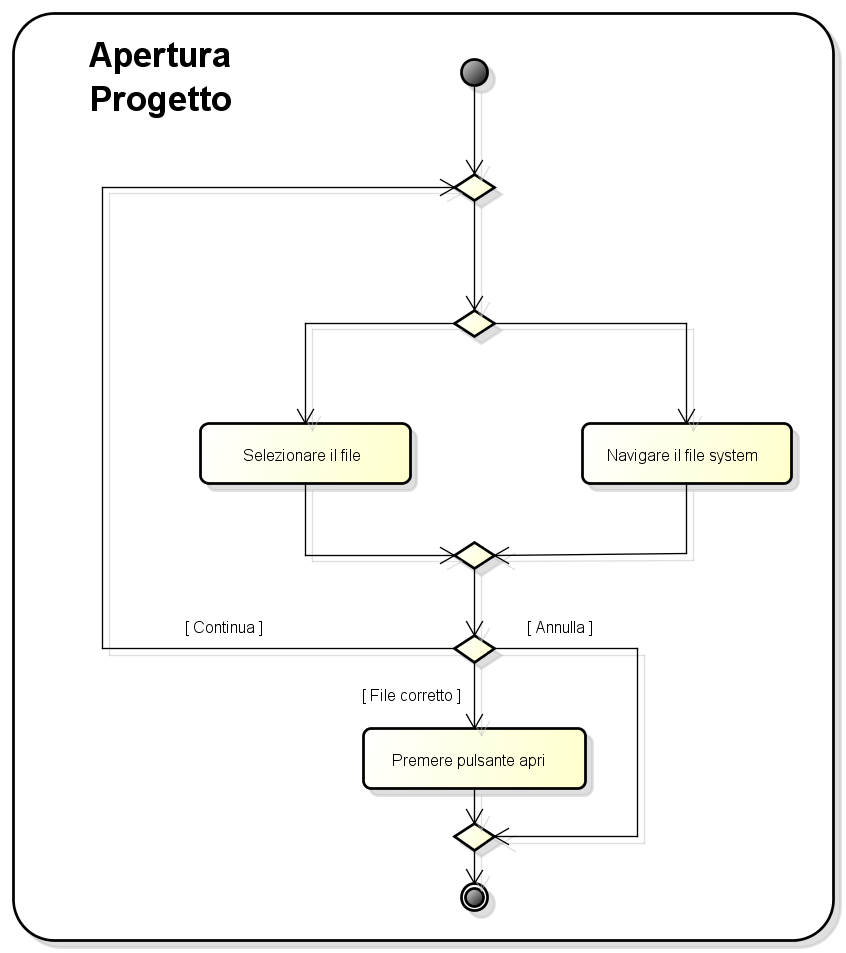
\includegraphics[scale=0.3] {img/activity_apertura.png} 
	\caption{Diagramma attività - Apertura di un progetto} 
\end{figure}
L'attività di apertura di un progetto in figura 8 permette all'utente di navigare il file system e di scegliere quale progetto deve essere aperto.
\newpage

\subsection{Modifica di un progetto}
\begin{figure}[h] 
	\centering 
	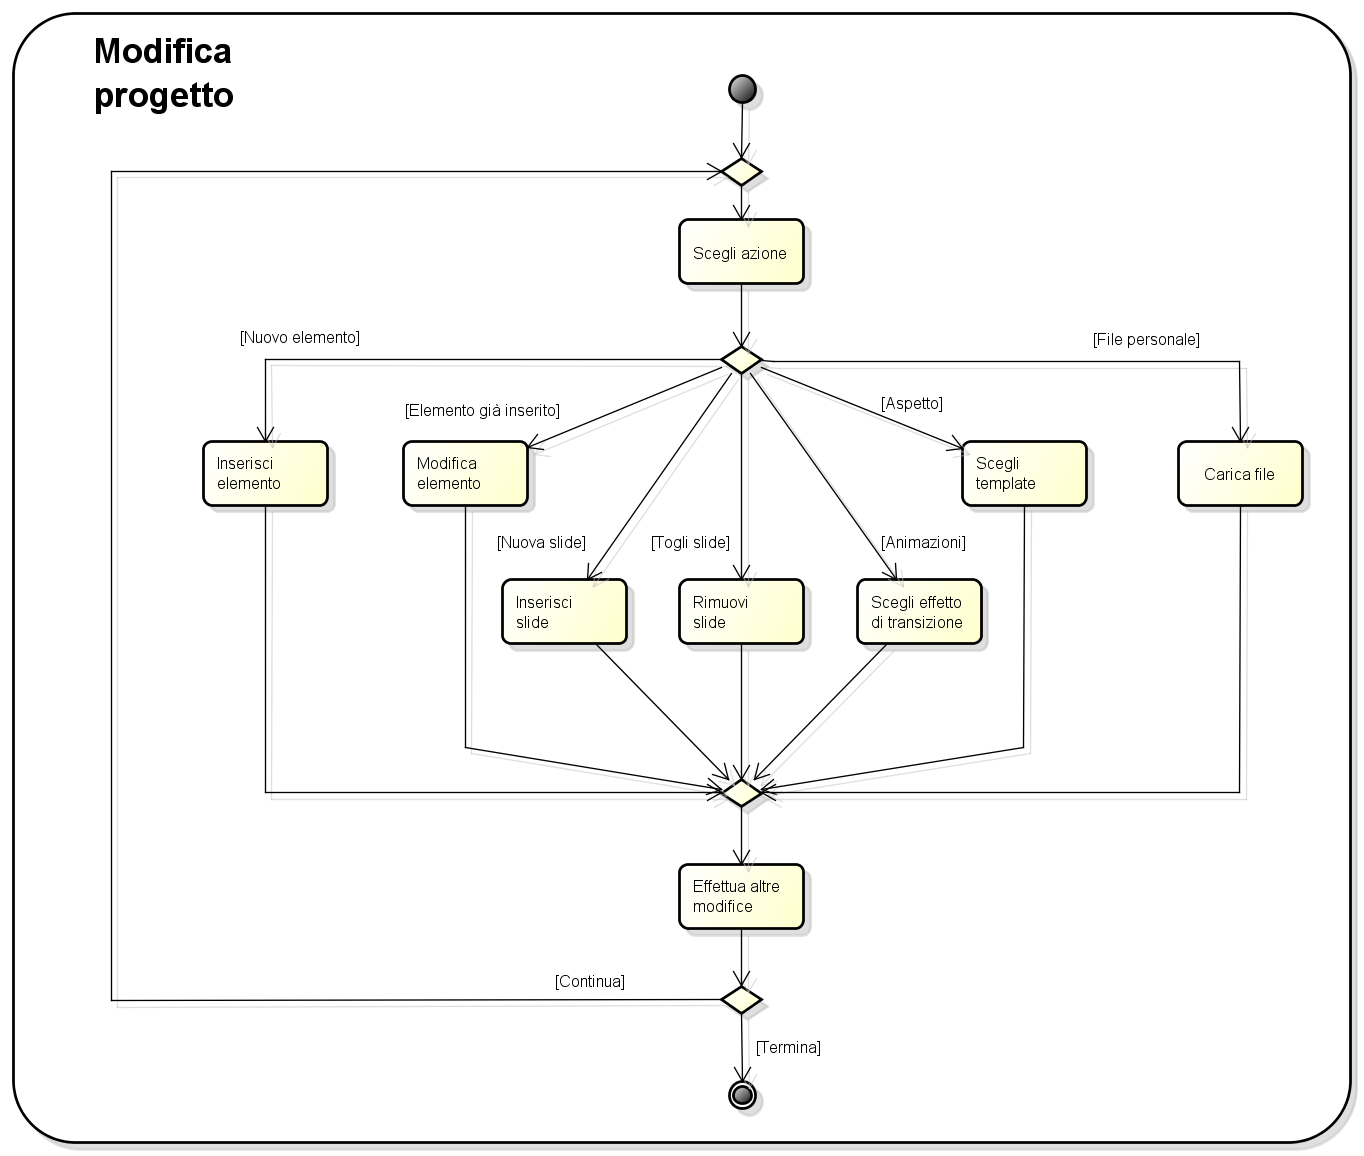
\includegraphics[scale=0.3] {img/activity_modifica.png} 
	\caption{Diagramma attività - Modifica di un progetto} 
\end{figure}
L'attività di modifica in figura 9 permette all'utente di inserire e modificare elementi (come testo, immagini, grafici, ecc...) nella presentazione corrente. L'utente può inoltre aggiungere e rimuovere slide, scegliere un diverso template e cambiare l'effetto di transizione tra una slide e l'altra.
\newpage

\subsection{Salvataggio di un progetto}
\begin{figure}[h] 
	\centering 
	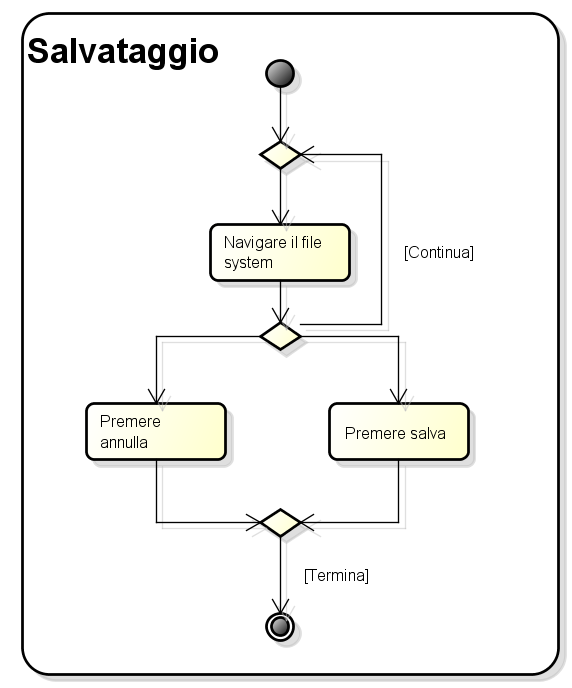
\includegraphics[scale=0.3] {img/activity_salvataggio.png} 
	\caption{Diagramma attività - Salvataggio di un progetto} 
\end{figure}
La figura 10 rappresenta l'attività di salvataggio di un progetto. Lo schema indica la possibilità per l'utente di navigare il file system e di scegliere un nome per il progetto da salvare o di selezionare un progetto già esistente da sovrascrivere.
\newpage
\newpage

\section{Tracciamento}
Per chiarezza si fa notare che tutte le classi riportate nelle tabelle di tracciamento si intendono appartenenti al package Premi.

	\begin{table}[h]
		\caption{Tabella del tracciamento requisiti-componenti}
		\begin{tabular}{|p{0.18\textwidth}|p{0.20\textwidth}|p{0.59\textwidth}|}
			\toprule
			
			\textbf{Requisito} & \textbf{Descrizione} & \textbf{Componente} \\
			
			\midrule

			R[OBB][F]1 & Il sistema deve permettere ad un utente la registrazione & Back-End::Logic-Tier::Controller::UsersController; Back-End::Logic-Tier::Controller; Back-End::Logic-Tier::Model; Back-End::Data-Tier; Front-End::Views::UsersView; Front-End::Controller; Front-End::Controller::UserController\\ \midrule
			R[OBB][F]1.1 & Il sistema deve permettere la scelta di un nome utente & Back-End::Logic-Tier::Controller::UsersController; Back-End::Logic-Tier::Controller; Back-End::Logic-Tier::Model; Back-End::Data-Tier; Front-End::Views::UsersView; Front-End::Controller; Front-End::Controller::UserController \\ \midrule
			R[OBB][F]1.1.1 & Il nome utente deve contenere almeno un carattere & Back-End::Logic-Tier::Controller::UsersController; Back-End::Logic-Tier::Controller; Back-End::Logic-Tier::Model; Back-End::Data-Tier; Front-End::Views::UsersView; Front-End::Controller; Front-End::Controller::UserController \\ \midrule
			R[OBB][F]1.1.2 & Il nome utente deve essere univoco & Back-End::Logic-Tier::Controller::UsersController; Back-End::Logic-Tier::Controller; Back-End::Logic-Tier::Model; Back-End::Data-Tier; Front-End::Views::UsersView; Front-End::Controller; Front-End::Controller::UserController \\ \midrule
			R[OBB][F]1.2 & Il sistema deve permettere la scelta di una password & Back-End::Logic-Tier::Controller::UsersController; Back-End::Logic-Tier::Controller; Back-End::Logic-Tier::Model; Back-End::Data-Tier; Front-End::Views::UsersView; Front-End::Controller; Front-End::Controller::UserController \\ \midrule
			R[OBB][F]1.2.1 & La password deve contenere almeno 8 caratteri & Back-End::Logic-Tier::Controller::UsersController; Back-End::Logic-Tier::Controller; Back-End::Logic-Tier::Model; Back-End::Data-Tier; Front-End::Views::UsersView; Front-End::Controller; Front-End::Controller::UserController \\ \midrule
			R[OBB][F]1.2.2 & La password deve essere criptata per garantire la confidenzialità dei dati & Back-End::Logic-Tier::Controller::UsersController; Back-End::Logic-Tier::Controller; Back-End::Logic-Tier::Model; Back-End::Data-Tier; Front-End::Views::UsersView; Front-End::Controller; Front-End::Controller::UserController \\ \midrule
			
	\end{tabular}
	\end{table}
	\newpage
	
	\begin{table}[h]
		\begin{tabular}{|p{0.18\textwidth}|p{0.20\textwidth}|p{0.59\textwidth}|}
			\midrule
			R[OBB][F]1.3 & Il sistema deve permettere l'inserimento del nome dell'utente & Back-End::Logic-Tier::Controller::UsersController; Back-End::Logic-Tier::Controller; Back-End::Logic-Tier::Model; Back-End::Data-Tier; Front-End::Views::UsersView; Front-End::Controller; Front-End::Controller::UserController \\ \midrule
			R[OBB][F]1.3.1 & Il nome deve contenere solo caratteri alfabetici & Back-End::Logic-Tier::Controller::UsersController; Back-End::Logic-Tier::Controller; Back-End::Logic-Tier::Model; Back-End::Data-Tier; Front-End::Views::UsersView; Front-End::Controller; Front-End::Controller::UserController \\ \midrule
			R[OBB][F]1.4 & Il sistema deve permettere l'inserimento del cognome dell'utente & Back-End::Logic-Tier::Controller::UsersController; Back-End::Logic-Tier::Controller; Back-End::Logic-Tier::Model; Back-End::Data-Tier; Front-End::Views::UsersView; Front-End::Controller; Front-End::Controller::UserController \\ \midrule
			R[OBB][F]1.4.1 & Il cognome deve contenere solo caratteri alfabetici & Back-End::Logic-Tier::Controller::UsersController ; Back-End::Logic-Tier::Controller ; Back-End::Logic-Tier::Model ; Back-End::Data-Tier ; Front-End::Views::UsersView ; Front-End::Controller ; Front-End::Controller::UserController \\ \midrule
			R[OBB][F]1.5 & Il sistema deve permettere l'inserimento di una email & Back-End::Logic-Tier::Controller::UsersController ; Back-End::Logic-Tier::Controller ; Back-End::Logic-Tier::Model ; Back-End::Data-Tier ; Front-End::Views::UsersView ; Front-End::Controller ; Front-End::Controller::UserController \\ \midrule
			R[OBB][F]1.5.1 & La mail deve essere formata da una stringa seguita dal carattere @ e una stringa dopo & Back-End::Logic-Tier::Controller::UsersController ; Back-End::Logic-Tier::Controller ; Back-End::Logic-Tier::Model ; Back-End::Data-Tier ; Front-End::Views::UsersView ; Front-End::Controller ; Front-End::Controller::UserController \\ \midrule
			R[OPZ][F]1.6 & Il sistema deve permettere la registrazione attraverso social network & Back-End::Logic-Tier::Controller::UsersController ; Back-End::Logic-Tier::Controller ; Back-End::Logic-Tier::Model ; Back-End::Data-Tier ; Front-End::Views::UsersView ; Front-End::Controller ; Front-End::Controller::UserController \\ \midrule
			R[OPZ][F]1.6.1 & Il sistema deve permettere la registrazione attraverso Facebook & Back-End::Logic-Tier::Controller::UsersController ; Back-End::Logic-Tier::Controller ; Back-End::Logic-Tier::Model ; Back-End::Data-Tier ; Front-End::Views::UsersView ; Front-End::Controller ; Front-End::Controller::UserController \\ \midrule
			R[OPZ][F]1.6.2 & Il sistema deve permettere la registrazione attraverso Twitter & Back-End::Logic-Tier::Controller::UsersController ; Back-End::Logic-Tier::Controller ; Back-End::Logic-Tier::Model ; Back-End::Data-Tier ; Front-End::Views::UsersView ; Front-End::Controller ; Front-End::Controller::UserController \\ \midrule
			
		\end{tabular}
		\end{table}
		\newpage
			
	\begin{table}[h]
		\begin{tabular}{|p{0.18\textwidth}|p{0.20\textwidth}|p{0.59\textwidth}|}
			\midrule	
			
			R[OPZ][F]1.6.3 & Il sistema deve permettere la registrazione attraverso Google+ & Back-End::Logic-Tier::Controller::UsersController ; Back-End::Logic-Tier::Controller ; Back-End::Logic-Tier::Model ; Back-End::Data-Tier ; Front-End::Views::UsersView ; Front-End::Controller ; Front-End::Controller::UserController \\ \midrule
			R[OPZ][F]1.6.1.1 & Il sistema deve permettere la visualizzazione di un messaggio di errore nel caso di mancata registrazione tramite Facebook & Back-End::Logic-Tier::Controller::UsersController ; Back-End::Logic-Tier::Controller ; Back-End::Logic-Tier::Model ; Back-End::Data-Tier ; Front-End::Views::UsersView ; Front-End::Controller ; Front-End::Controller::UserController \\ \midrule
			R[OPZ][F]1.6.2.1 & Il sistema deve permettere la visualizzazione di un messaggio di errore nel caso di mancata registrazione tramite Twitter & Back-End::Logic-Tier::Controller::UsersController ; Back-End::Logic-Tier::Controller ; Back-End::Logic-Tier::Model ; Back-End::Data-Tier ; Front-End::Views::UsersView ; Front-End::Controller ; Front-End::Controller::UserController \\ \midrule
			R[OPZ][F]1.6.3.1 & Il sistema deve permettere la visualizzazione di un messaggio di errore nel caso di mancata registrazione tramite Google+ & Back-End::Logic-Tier::Controller::UsersController ; Back-End::Logic-Tier::Controller ; Back-End::Logic-Tier::Model ; Back-End::Data-Tier ; Front-End::Views::UsersView ; Front-End::Controller ; Front-End::Controller::UserController \\ \midrule
			R[OPZ][F]1.6.4 & Il sistema deve permettere la visualizzazione di avvenuta registrazione  & Back-End::Logic-Tier::Controller::UsersController ; Back-End::Logic-Tier::Controller ; Back-End::Logic-Tier::Model ; Back-End::Data-Tier ; Front-End::Views::UsersView ; Front-End::Controller ; Front-End::Controller::UserController \\ \midrule
			R[OBB][F]1.7 & Il sistema deve permettere la visualizzazione di un messaggio di errore se i campi richiesti risultano sbagliati & Back-End::Logic-Tier::Controller::UsersController ; Back-End::Logic-Tier::Controller ; Back-End::Logic-Tier::Model ; Back-End::Data-Tier ; Front-End::Views::UsersView ; Front-End::Controller ; Front-End::Controller::UserController \\ \midrule
			R[OBB][F]2 & Il sistema deve permettere l'autenticazione dell'utente & Back-End::Logic-Tier::Controller::UsersController ; Back-End::Logic-Tier::Controller ; Back-End::Logic-Tier::Model ; Back-End::Data-Tier ; Front-End::Views::UsersView ; Front-End::Controller ; Front-End::Controller::UserController \\ \midrule
			R[OBB][F]2.1 & Il sistema deve permettere l'inserimento del nome utente & Back-End::Logic-Tier::Controller::UsersController ; Back-End::Logic-Tier::Controller ; Back-End::Logic-Tier::Model ; Back-End::Data-Tier ; Front-End::Views::UsersView ; Front-End::Controller ; Front-End::Controller::UserController \\ \midrule
			R[OBB][F]2.2 & Il sistema deve permettere l'inserimento della password & Back-End::Logic-Tier::Controller::UsersController ; Back-End::Logic-Tier::Controller ; Back-End::Logic-Tier::Model ; Back-End::Data-Tier ; Front-End::Views::UsersView ; Front-End::Controller ; Front-End::Controller::UserController \\ \midrule
	
	\end{tabular}
	\end{table}
	\newpage
	
	\begin{table}[h]
			\begin{tabular}{|p{0.18\textwidth}|p{0.20\textwidth}|p{0.59\textwidth}|}
			\midrule
	
			
			R[OBB][F]2.3 & Il sistema deve segnalare l'errato inserimento delle credenziali & Back-End::Logic-Tier::Controller::UsersController ; Back-End::Logic-Tier::Controller ; Back-End::Logic-Tier::Model ; Back-End::Data-Tier ; Front-End::Views::UsersView ; Front-End::Controller ; Front-End::Controller::UserController \\ \midrule
			R[OBB][F]2.4 & Il sistema deve permettere il reindirizzamento alla pagina personale in caso di avvenuta autenticazione & Back-End::Logic-Tier::Controller::UsersController ; Back-End::Logic-Tier::Controller ; Back-End::Logic-Tier::Model ; Back-End::Data-Tier ; Front-End::Views::UsersView ; Front-End::Controller ; Front-End::Controller::UserController \\ \midrule
			R[OBB][F]2.5 & Il sistema deve permettere il recupero della password e del nome utente in caso di dimenticanza & Back-End::Logic-Tier::Controller::UsersController ; Back-End::Logic-Tier::Controller ; Back-End::Logic-Tier::Model ; Back-End::Data-Tier ; Front-End::Views::UsersView ; Front-End::Controller ; Front-End::Controller::UserController \\ \midrule
			R[OBB][F]2.5.1 & Il sistema deve permettere l'inserimento delle email per il recupero della password e del nome utente & Back-End::Logic-Tier::Controller::UsersController ; Back-End::Logic-Tier::Controller ; Back-End::Logic-Tier::Model ; Back-End::Data-Tier ; Front-End::Views::UsersView ; Front-End::Controller ; Front-End::Controller::UserController \\ \midrule
			R[OBB][F]3 & Il sistema deve permettere la ricerca di un progetto  & Back-End::Logic-Tier::Controller ; Back-End::Logic-tier::UsersController ; Back-End::Data-Tier ; Front-End::Views ; Front-End::Controller \\ \midrule
			R[OBB][F]3.1 & Il sistema deve permettere la ricerca attraverso l'inserimento del nome utente & Back-End::Logic-Tier::Controller ; Back-End::Logic-tier::UsersController ; Back-End::Data-Tier ; Front-End::Views ; Front-End::Controller \\ \midrule
			R[OBB][F]3.2 & Il sistema deve permettere la ricerca attraverso l'inserimento del titolo del progetto & Back-End::Logic-Tier::Controller ; Back-End::Logic-tier::UsersController ; Back-End::Data-Tier ; Front-End::Views ; Front-End::Controller \\ \midrule
			R[OBB][F]3.3 & Il sistema deve permettere la visualizzazione del risultato della ricerca & Back-End::Logic-Tier::Controller ; Back-End::Logic-tier::UsersController ; Back-End::Data-Tier ; Front-End::Views ; Front-End::Controller \\ \midrule
			R[OBB][F]3.4 & Il sistema deve permettere il reinserimento di un nome utente diverso per la ricerca & Back-End::Logic-Tier::Controller ; Back-End::Logic-tier::UsersController ; Back-End::Data-Tier ; Front-End::Views ; Front-End::Controller \\ \midrule
			R[OBB][F]3.5 & Il sistema deve permettere il reinserimento di un titolo diverso per la ricerca & Back-End::Logic-Tier::Controller ; Back-End::Logic-tier::UsersController ; Back-End::Data-Tier ; Front-End::Views ; Front-End::Controller \\ \midrule

		\end{tabular}
	\end{table}
	\newpage
	
	\begin{table}[h]
		\begin{tabular}{|p{0.18\textwidth}|p{0.20\textwidth}|p{0.59\textwidth}|}
			\midrule
			
			R[OBB][F]4 & Il sistema deve permettere all'utente l'apertura del progetto in modalità visualizzazione & Back-End::Logic-Tier::Controller; Back-End::Logic-Tier::Model::ProjectModel; Back-End::Data-Tier; Front-End::Model; Front-End::Views::PresentSlideShowViews ; Front-End::Controller::PresentSlideShowController; \\ \midrule
			R[OBB][F]4.1 & Il sistema deve permettere all'utente l'apertura di una presentazione & Back-End::Logic-Tier::Controller ; Back-End::Logic-Tier::Model::ProjectModel ; Back-End::Data-Tier ; Front-End::Model ; Front-End::Views::PresentSlideShowViews ; Front-End::Controller::PresentSlideShowController; \\ \midrule
			R[OBB][F]4.1.1 & Il sistema deve permettere all'utente autenticato la visualizzazione di una presentazione in modalità presentatore & Back-End::Logic-Tier::Controller  ; Back-End::Logic-Tier::Model::ProjectModel ; Back-End::Data-Tier ; Front-End::Model ; Front-End::Views::PresentSlideShowViews ; Front-End::Controller::PresentSlideShowController ; Back-End::Presentation-Tier \\ \midrule
			R[OBB][F]4.1.1.1 & Il sistema deve poter visualizzare la slide corrente per il presentatore & Back-End::Logic-Tier::Controller ; Back-End::Logic-Tier::Model::ProjectModel ; Back-End::Data-Tier ; Front-End::Model ; Front-End::Views::PresentSlideShowViews ; Front-End::Controller::PresentSlideShowController ; Back-End::Presentation-Tier \\ \midrule
			R[OBB][F]4.1.1.2 & Il sistema deve poter visualizzare le slide successive per il presentatore & Back-End::Logic-Tier::Controller ; Back-End::Logic-Tier::Model::ProjectModel ; Back-End::Data-Tier ; Front-End::Model ; Front-End::Views::PresentSlideShowViews ; Front-End::Controller::PresentSlideShowController ; Back-End::Presentation-Tier \\ \midrule
			R[OBB][F]4.1.1.3 & Il sistema deve poter visualizzare le note della slide per il presentatore & Back-End::Logic-Tier::Controller ; Back-End::Logic-Tier::Controller ; Back-End::Logic-Tier::Model::ProjectModel ; Back-End::Data-Tier ; Front-End::Model ; Front-End::Views::PresentSlideShowViews ; Front-End::Controller::PresentSlideShowController ; Back-End::Presentation-Tier \\ \midrule
			R[OBB][F]4.1.1.4 & Il sistema deve poter visualizzare il tempo trascorso per il presentatore & Back-End::Logic-Tier::Controller ; Back-End::Logic-Tier::Controller ; Back-End::Logic-Tier::Model::ProjectModel ; Back-End::Data-Tier ; Front-End::Model ; Front-End::Views::PresentSlideShowViews ; Front-End::Controller::PresentSlideShowController ; Back-End::Presentation-Tier \\ \midrule
			R[OBB][F]4.1.1.5 & Il sistema deve poter visualizzare il tempo trascorso per il presentatore & Back-End::Logic-Tier::Controller ; Back-End::Logic-Tier::Controller ; Back-End::Logic-Tier::Model::ProjectModel ; Back-End::Data-Tier ; Front-End::Model ; Front-End::Views::PresentSlideShowViews ; Front-End::Controller::PresentSlideShowController ; Back-End::Presentation-Tier \\ \midrule

		\end{tabular}
	\end{table}
	\newpage
	
	\begin{table}[h]
		\begin{tabular}{|p{0.18\textwidth}|p{0.20\textwidth}|p{0.59\textwidth}|}
			\midrule
			
			R[OBB][F]4.1.2 & Il sistema deve permettere all'utente autenticato la visualizzazione di una presentazione in modalità ascoltatore & Back-End::Logic-Tier::Controller ; Back-End::Logic-Tier::Model::ProjectModel ; Back-End::Presentation-Tier ; Front-End::Views::PresentSlideShowView ; Front-End::Model; Front-End::Controller::PresentSlideShowController \\ \midrule
			R[OBB][F]4.1.2.1 & Il sistema deve poter visualizzare la slide corrente per l'ascoltatore & Back-End::Logic-Tier::Controller ; Back-End::Logic-Tier::Model::ProjectModel ; Back-End::Presentation-Tier ; Front-End::Views::PresentSlideShowView ; Front-End::Model; Front-End::Controller::PresentSlideShowController \\ \midrule
			R[OBB][F]4.1.3 & Il sistema deve poter visualizzare i comandi di navigazione per l'ascoltatore & Back-End::Logic-Tier::Controller ; Back-End::Logic-Tier::Model::ProjectModel ; Back-End::Presentation-Tier ; Front-End::Views::PresentSlideShowView ; Front-End::Model; Front-End::Controller::PresentSlideShowController \\ \midrule
			R[OPZ][F]4.2 & Il sistema deve permettere all'utente la visualizzazione di un'infografica & Back-End::Logic-Tier ; Back-End::Logic-Tier::Model::ProjectModel; Back-End::Data-Tier ; Front-End::Views::InfographicEditorViews ; Front-End::Model ; Front-End::Controller::InfographicEditorController ;   \\ \midrule
			R[OBB][F]5 & Il sistema deve permettere all'utente di generare il PDF del progetto & Back-End::Logic-Tier::Controller ; Back-End::Logic-Tier::Model::ProjectModel ; Front-End::Views ; Front-End::Controller \\ \midrule
			R[OBB][F]5.1 & Il sistema deve permettere all'utente di generare il PDF della presentazione & Back-End::Logic-Tier::Controller ; Back-End::Logic-Tier::Model::ProjectModel ; Front-End::Views ; Front-End::Controller \\ \midrule
			R[OBB][F]5.2 & Il sistema deve permettere all'utente di generare il PDF dell'infografica & Back-End::Logic-Tier::Controller ; Back-End::Logic-Tier::Model::ProjectModel ; Front-End::Views ; Front-End::Controller \\ \midrule
			R[OBB][F]6 & L'utente deve poter esportare un pacchetto stand-alone per la visualizzazione offline & Back-End::Logic-Tier::Controller ; Back-End::Logic-Tier::Model::ProjectModel ; Front-End::Views ; Front-End::Controller \\ \midrule
			R[OBB][F]6.1 & L'utente deve poter scegliere il percorso per il salvataggio del pacchetto & Back-End::Logic-Tier::Controller ; Back-End::Logic-Tier::Model::ProjectModel ; Front-End::Views ; Front-End::Controller \\ \midrule

		\end{tabular}
	\end{table}
	\newpage
	
	\begin{table}[h]
		\begin{tabular}{|p{0.18\textwidth}|p{0.20\textwidth}|p{0.59\textwidth}|}
			\midrule

				R[OBB][F]7 & L'utente deve poter creare un nuovo progetto & Back-End::Logic-Tier::Controller ; Back-End::Logic-Tier::Model::ProjectModel ; Front-End::Views ; Front-End::Controller \\ \midrule
				R[OBB][F]7.1 & L'utente deve poter inserire il titolo del progetto & Back-End::Logic-Tier::Controller ; Back-End::Logic-Tier::Model::ProjectModel ; Front-End::Views ; Front-End::Controller \\ \midrule
				R[OBB][F]7.2 & L'utente deve poter scegliere il template di stile per il proprio progetto & Back-End::Logic-Tier::Controller ; Back-End::Logic-Tier::Model::ProjectModel ; Front-End::Views ; Front-End::Model ; Front-End::Controller \\ \midrule
				R[OBB][F]8 & Il proprietario deve poter aprire un progetto da lui precedentemente creato & Back-End::Logic-Tier::Controller ; Back-End::Logic-Tier::Model::ProjectModel ; Back-End::Data-Tier ; Front-End::Views ; Front-End::Model ; Front-End::Controller \\ \midrule
				R[OBB][F]8.1 & Il proprietario deve poter scegliere il progetto da aprire & Back-End::Logic-Tier::Controller ; Back-End::Logic-Tier::Model::ProjectModel ; Back-End::Data-Tier ; Front-End::Views ; Front-End::Model ; Front-End::Controller \\ \midrule
				R[OBB][F]9 & Il proprietario deve poter modificare il contenuto di una slide & Back-End::Logic-Tier::Controller ; Back-End::Logic-Tier::Model::ProjectModel ; Back-End::Data-Tier ; Front-End::Views ; Front-End::Model ; Front-End::Controllero \\ \midrule
				R[OBB][F]9.1 & Il proprietario deve poter modificare il template di stile della presentazione & Back-End::Logic-Tier::Controller ; Back-End::Logic-Tier::Model::ProjectModel ; Back-End::Data-Tier ; Front-End::Views ; Front-End::Model ; Front-End::Controller \\ \midrule
				R[OBB][F]9.2 & Il proprietario deve poter inserire una nuova slide & Back-End::Logic-Tier::Controller ; Back-End::Logic-Tier::Model::ProjectModel ; Back-End::Data-Tier ; Front-End::Views ; Front-End::Model ; Front-End::Controller \\ \midrule
				R[OBB][F]9.2.1 & Il proprietario deve poter inserire una nuova slide a destra & Back-End::Logic-Tier::Controller ; Back-End::Logic-Tier::Model::ProjectModel ; Back-End::Data-Tier ; Front-End::Views ; Front-End::Model ; Front-End::Controller \\ \midrule
				R[OBB][F]9.2.2 & Il proprietario deve poter inserire una nuova slide a sinistra & Back-End::Logic-Tier::Controller ; Back-End::Logic-Tier::Model::ProjectModel ; Back-End::Data-Tier ; Front-End::Views ; Front-End::Model ; Front-End::Controller \\ \midrule
				R[OBB][F]9.3 & Il proprietario deve poter rimuovere una slide & Back-End::Logic-Tier::Controller ; Back-End::Logic-Tier::Model::ProjectModel ; Back-End::Data-Tier ; Front-End::Views ; Front-End::Model ; Front-End::Controller \\ \midrule

		\end{tabular}
	\end{table}
	\newpage
	
	\begin{table}[h]
		\begin{tabular}{|p{0.18\textwidth}|p{0.20\textwidth}|p{0.59\textwidth}|}
			\midrule
			
			R[OBB][F]9.4 & Il proprietario deve poter inserire un immagine & Back-End::Logic-Tier::Controller ; Back-End::Logic-Tier::Model::ProjectModel ; Back-End::Data-Tier ; Front-End::Views ; Front-End::Model ; Front-End::Controller \\ \midrule
			R[OBB][F]9.4.1 & Il sistema deve accettare in input immagini di formato JPG & Back-End::Logic-Tier::Controller ; Back-End::Logic-Tier::Model::ProjectModel ; Back-End::Data-Tier ; Front-End::Views ; Front-End::Model ; Front-End::Controller \\ \midrule
			R[OBB][F]9.4.2 & Il sistema deve accettare in input immagini di formato PNG & Back-End::Logic-Tier::Controller ; Back-End::Logic-Tier::Model::ProjectModel ; Back-End::Data-Tier ; Front-End::Views ; Front-End::Model ; Front-End::Controller \\ \midrule
			R[OBB][F]9.4.3 & Il sistema deve accettare in input immagini di formato GIF & Back-End::Logic-Tier::Controller ; Back-End::Logic-Tier::Model::ProjectModel ; Back-End::Data-Tier ; Front-End::Views ; Front-End::Model ; Front-End::Controller \\ \midrule
			R[OBB][F]9.5 & Il proprietario deve poter inserire elementi di testo & Back-End::Logic-Tier::Controller ; Back-End::Logic-Tier::Model::ProjectModel ; Back-End::Data-Tier ; Front-End::Views ; Front-End::Model ; Front-End::Controller \\ \midrule
			R[OPZ][F]9.6 & Il proprietario deve poter inserire dati real time & Back-End::Logic-Tier::Controller ; Back-End::Logic-Tier::Model::ProjectModel ; Back-End::Data-Tier ; Front-End::Views ; Front-End::Model ; Front-End::Controller \\ \midrule
			R[OPZ][F]9.6.1 & Il proprietario deve poter caricare un file di dati & Back-End::Logic-Tier::Controller ; Back-End::Logic-Tier::Model::ProjectModel ; Back-End::Data-Tier ; Front-End::Views ; Front-End::Model ; Front-End::Controller \\ \midrule
			R[OPZ][F]9.6.2 & Il proprietario deve poter caricare un file per la funzione di estrapolazione dati & Back-End::Logic-Tier::Controller ; Back-End::Logic-Tier::Model::ProjectModel ; Back-End::Data-Tier ; Front-End::Views ; Front-End::Model ; Front-End::Controller \\ \midrule
			R[OPZ][F]9.6.3 & Il proprietario deve poter caricare un file per la funzione di elaborazione di dati dall'array & Back-End::Logic-Tier::Controller ; Back-End::Logic-Tier::Model::ProjectModel ; Back-End::Data-Tier ; Front-End::Views ; Front-End::Model ; Front-End::Controller \\ \midrule
			R[OPZ][F]9.6.4 & Il proprietario deve poter scegliere il tipo di dati real time da inserire & Back-End::Logic-Tier::Controller ; Back-End::Logic-Tier::Model::ProjectModel ; Back-End::Data-Tier ; Front-End::Views ; Front-End::Model ; Front-End::Controller \\ \midrule
			R[OPZ][F]9.6.5 & Il proprietario deve poter scegliere la sorgente di dati real time & Back-End::Logic-Tier::Controller ; Back-End::Logic-Tier::Model::ProjectModel ; Back-End::Data-Tier ; Front-End::Views ; Front-End::Model ; Front-End::Controller \\ \midrule

		\end{tabular}
	\end{table}
	\newpage
	
	\begin{table}[h]
		\begin{tabular}{|p{0.18\textwidth}|p{0.20\textwidth}|p{0.59\textwidth}|}
			\midrule

			R[OBB][F]9.7 & Il proprietario deve poter inserire le tabelle & Back-End::Logic-Tier::Controller ; Back-End::Logic-Tier::Model::ProjectModel ; Back-End::Data-Tier ; Front-End::Views ; Front-End::Model ; Front-End::Controller \\ \midrule
			R[OBB][F]9.7.1 & Il proprietario deve poter scegliere il numero di righe della tabella & Back-End::Logic-Tier::Controller ; Back-End::Logic-Tier::Model::ProjectModel ; Back-End::Data-Tier ; Front-End::Views ; Front-End::Model ; Front-End::Controller \\ \midrule
			R[OBB][F]9.7.2 & Il proprietario deve poter scegliere il numero di colonne della tabella & Back-End::Logic-Tier::Controller ; Back-End::Logic-Tier::Model::ProjectModel ; Back-End::Data-Tier ; Front-End::Views ; Front-End::Model ; Front-End::Controller \\ \midrule
			R[OPZ][F]9.8 & Il proprietario deve poter inserire un grafico & Back-End::Logic-Tier::Controller ; Back-End::Logic-Tier::Model::ProjectModel ; Back-End::Data-Tier ; Front-End::Views ; Front-End::Model ; Front-End::Controller \\ \midrule
			R[OPZ][F]9.8.1 & Il proprietario deve poter scegliere il modello di grafico & Back-End::Logic-Tier::Controller ; Back-End::Logic-Tier::Model::ProjectModel ; Back-End::Data-Tier ; Front-End::Views ; Front-End::Model ; Front-End::Controller \\ \midrule
			R[OPZ][F]9.8.1.1 & Il proprietario deve poter scegliere il modello di grafico istogramma & Back-End::Logic-Tier::Controller ; Back-End::Logic-Tier::Model::ProjectModel ; Back-End::Data-Tier ; Front-End::Views ; Front-End::Model ; Front-End::Controller \\ \midrule
			R[OPZ][F]9.8.1.2 & Il proprietario deve poter scegliere il modello di grafico a torta & Back-End::Logic-Tier::Controller ; Back-End::Logic-Tier::Model::ProjectModel ; Back-End::Data-Tier ; Front-End::Views ; Front-End::Model ; Front-End::Controller \\ \midrule
			R[OPZ][F]9.8.1.3 & Il proprietario deve poter scegliere il modello di grafico a linea & Back-End::Logic-Tier::Controller ; Back-End::Logic-Tier::Model::ProjectModel ; Back-End::Data-Tier ; Front-End::Views ; Front-End::Model ; Front-End::Controller \\ \midrule
			R[OPZ][F]9.8.2 & Il proprietario deve poter inserire il numero di elementi che avrà il grafico & Back-End::Logic-Tier::Controller ; Back-End::Logic-Tier::Model::ProjectModel ; Back-End::Data-Tier ; Front-End::Views ; Front-End::Model ; Front-End::Controller \\ \midrule
			R[OPZ][F]9.8.3 & Il proprietario deve poter inserire il nome degli elementi del grafico  & Back-End::Logic-Tier::Controller ; Back-End::Logic-Tier::Model::ProjectModel ; Back-End::Data-Tier ; Front-End::Views ; Front-End::Model ; Front-End::Controller \\ \midrule
			R[OPZ][F]9.8.4 & Il proprietario deve poter inserire il valore degli elementi del grafico & Back-End::Logic-Tier::Controller ; Back-End::Logic-Tier::Model::ProjectModel ; Back-End::Data-Tier ; Front-End::Views ; Front-End::Model ; Front-End::Controller \\ \midrule

	\end{tabular}
	\end{table}
	\newpage
	
	\begin{table}[h]
		\begin{tabular}{|p{0.18\textwidth}|p{0.20\textwidth}|p{0.59\textwidth}|}
			\midrule
	
			R[OBB][F]9.9 & Il proprietario deve poter scegliere un effetto di transizione delle slide & Back-End::Presentation-Tier ; Back-End::Logic-Tier::Controller ; Back-End::Logic-Tier::Model::ProjectModel ; Back-End::Data-Tier ; Front-End::Views::PresentSlideShowViews ; Front-End::Controller::PresentSlideShowController \\ \midrule
			R[OBB][F]9.9.1 & Il proprietario deve poter scegliere l'effetto di transizione a scorrimento & Back-End::Presentation-Tier ; Back-End::Logic-Tier::Controller ; Back-End::Logic-Tier::Model::ProjectModel ; Back-End::Data-Tier ; Front-End::Views::PresentSlideShowViews ; Front-End::Controller::PresentSlideShowController \\ \midrule
			R[OBB][F]9.9.2 & Il proprietario deve poter scegliere l'effetto di transizione a dissolvenza & Back-End::Presentation-Tier ; Back-End::Logic-Tier::Controller ; Back-End::Logic-Tier::Model::ProjectModel ; Back-End::Data-Tier ; Front-End::Views::PresentSlideShowViews ; Front-End::Controller::PresentSlideShowController \\ \midrule
			R[OBB][F]9.9.3 & Il proprietario deve poter scegliere l'effetto di transizione a convesso & Back-End::Presentation-Tier ; Back-End::Logic-Tier::Controller ; Back-End::Logic-Tier::Model::ProjectModel ; Back-End::Data-Tier ; Front-End::Views::PresentSlideShowViews ; Front-End::Controller::PresentSlideShowController \\ \midrule
			R[OBB][F]9.9.4 & Il proprietario deve poter scegliere l'effetto di transizione a concavo & Back-End::Presentation-Tier ; Back-End::Logic-Tier::Controller ; Back-End::Logic-Tier::Model::ProjectModel ; Back-End::Data-Tier ; Front-End::Views::PresentSlideShowViews ; Front-End::Controller::PresentSlideShowController \\ \midrule
			R[OBB][F]9.9.5 & Il proprietario deve poter scegliere nessun effetto di transizione & Back-End::Presentation-Tier ; Back-End::Logic-Tier::Controller ; Back-End::Logic-Tier::Model::ProjectModel ; Back-End::Data-Tier ; Front-End::Views::PresentSlideShowViews ; Front-End::Controller::PresentSlideShowController \\ \midrule
			R[OBB][F]9.10 & Il proprietario deve poter ridimensionare un elemento selezionato & Back-End::Logic-Tier::Controller::ComponentController ; Back-End::Logic-Tier::Model::ProjectModel ; Front-End::Views ; Front-End::Model; Front-End::Controller  \\ \midrule
			R[OBB][F]9.11 & Il proprietario deve poter spostare un elemento selezionato & Back-End::Logic-Tier::Controller::ComponentController ; Back-End::Logic-Tier::Model::ProjectModel ; Front-End::Views ; Front-End::Model; Front-End::Controller  \\ \midrule
			R[OBB][F]9.12 & Il proprietario deve poter ruotare un elemento selezionato & Back-End::Logic-Tier::Controller::ComponentController; Back-End::Logic-Tier::Model::ProjectModel ; Front-End::Views ; Front-End::Model; Front-End::Controller  \\ \midrule
			R[OBB][F]9.13 & Il proprietario deve poter rimuovere un elemento selezionato & Back-End::Logic-Tier::Controller::ComponentController ; Back-End::Logic-Tier::Model::ProjectModel ; Front-End::Views ; Front-End::Model; Front-End::Controller \\ \midrule

		\end{tabular}	
		\end{table}
		\newpage

		
	\begin{table}[h]
		\begin{tabular}{|p{0.18\textwidth}|p{0.20\textwidth}|p{0.59\textwidth}|}
			\midrule
			
			R[OBB][F]9.14 & Il proprietario deve poter caricare un file da inserire nella slide & Back-End::Logic-Tier::Controller::ComponentController ; Back-End::Logic-Tier::Model::ProjectModel ; Front-End::Views ; Front-End::Model; Front-End::Controller  \\ \midrule
			R[OBB][F]9.15 & Il proprietario deve poter modificare la formattazione del testo & Back-End::Logic-Tier::Controller::ComponentController ; Back-End::Logic-Tier::Model::ProjectModel ; Front-End::Views ; Front-End::Model; Front-End::Controller  \\ \midrule
			R[OBB][F]9.15.1 & Il proprietario deve poter cambiare la grandezza del testo & Back-End::Logic-Tier::Controller::ComponentController ; Back-End::Logic-Tier::Model::ProjectModel ; Front-End::Views ; Front-End::Model; Front-End::Controller  \\ \midrule
			R[OBB][F]9.15.2 & Il proprietario deve poter cambiare il colore del testo & Back-End::Logic-Tier::Controller::ComponentController ; Back-End::Logic-Tier::Model::ProjectModel ; Front-End::Views ; Front-End::Model; Front-End::Controller  \\ \midrule
			R[OBB][F]9.15.3 & Il proprietario deve poter cambiare il font del testo & Back-End::Logic-Tier::Controller::ComponentController ; Back-End::Logic-Tier::Model::ProjectModel ; Front-End::Views ; Front-End::Model; Front-End::Controller  \\ \midrule
			R[OBB][F]9.15.4 & Il proprietario deve poter abilitare/disabilitare il corsivo del testo & Back-End::Logic-Tier::Controller::ComponentController ; Back-End::Logic-Tier::Model::ProjectModel ; Front-End::Views ; Front-End::Model; Front-End::Controller  \\ \midrule
			R[OBB][F]9.15.5 & Il proprietario deve poter abilitare/disabilitare il grassetto del testo & Back-End::Logic-Tier::Controller::ComponentController ; Back-End::Logic-Tier::Model::ProjectModel ; Front-End::Views ; Front-End::Model; Front-End::Controller  \\ \midrule
			R[OBB][F]9.15.6 & Il proprietario deve poter cambiare la posizione del testo all'interno della slide & Back-End::Logic-Tier::Controller::ComponentController ; Back-End::Logic-Tier::Model::ProjectModel ; Front-End::Views ; Front-End::Model; Front-End::Controller  \\ \midrule
			R[OBB][F]9.16 & Il proprietario deve poter modificare una tabella & Back-End::Logic-Tier::Controller::ComponentController ; Back-End::Logic-Tier::Model::ProjectModel ; Front-End::Views ; Front-End::Model; Front-End::Controller  \\ \midrule
			R[OBB][F]9.16.1 & Il proprietario deve poter cambiare il contenuto di una cella della tabella & Back-End::Logic-Tier::Controller::ComponentController ; Back-End::Logic-Tier::Model::ProjectModel ; Front-End::Views ; Front-End::Model; Front-End::Controller  \\ \midrule
			R[OBB][F]9.16.2 & Il proprietario deve poter aggiungere righe alla tabella & Back-End::Logic-Tier::Controller::ComponentController ; Back-End::Logic-Tier::Model::ProjectModel ; Front-End::Views ; Front-End::Model; Front-End::Controller  \\ \midrule
			
	\end{tabular}
		\end{table}
			\newpage
			
	\begin{table}[h]
		\begin{tabular}{|p{0.18\textwidth}|p{0.20\textwidth}|p{0.59\textwidth}|}
		\midrule
		
		R[OBB][F]9.16.3 & Il proprietario deve poter cancellare righe alla tabella & Back-End::Logic-Tier::Controller::ComponentController ; Back-End::Logic-Tier::Model::ProjectModel ; Front-End::Views ; Front-End::Model; Front-End::Controller  \\ \midrule
		R[OBB][F]9.16.4 & Il proprietario deve poter aggiungere colonne alla tabella & Back-End::Logic-Tier::Controller::ComponentController ; Back-End::Logic-Tier::Model::ProjectModel ; Front-End::Views ; Front-End::Model; Front-End::Controller  \\ \midrule
		R[OBB][F]9.16.5 & Il proprietario deve poter cancellare colonne alla tabella & Back-End::Logic-Tier::Controller::ComponentController ; Back-End::Logic-Tier::Model::ProjectModel ; Front-End::Views ; Front-End::Model; Front-End::Controller  \\ \midrule
		R[OBB][F]9.16.6 & Il proprietario deve poter modificare la grandezza della tabella & Back-End::Logic-Tier::Controller::ComponentController ; Back-End::Logic-Tier::Model::ProjectModel ; Front-End::Views ; Front-End::Model; Front-End::Controller  \\ \midrule
		R[OPZ][F]9.17 & Il proprietario deve poter modificare un grafico & Back-End::Logic-Tier::Controller::ComponentController ; Back-End::Logic-Tier::Model::ProjectModel ; Front-End::Views ; Front-End::Model; Front-End::Controller  \\ \midrule
		R[OPZ][F]9.17.1 & Il proprietario deve poter aggiungere un elemento al grafico & Back-End::Logic-Tier::Controller::ComponentController ; Back-End::Logic-Tier::Model::ProjectModel ; Front-End::Views ; Front-End::Model; Front-End::Controller  \\ \midrule
		R[OPZ][F]9.17.2 & Il proprietario deve poter cancellare un elemento dal grafico & Back-End::Logic-Tier::Controller::ComponentController ; Back-End::Logic-Tier::Model::ProjectModel ; Front-End::Views ; Front-End::Model; Front-End::Controller  \\ \midrule
		R[OPZ][F]9.17.3 & Il proprietario deve poter modificare il nome di un elemento del grafico & Back-End::Logic-Tier::Controller::ComponentController ; Back-End::Logic-Tier::Model::ProjectModel ; Front-End::Views ; Front-End::Model; Front-End::Controller  \\ \midrule
		R[OPZ][F]9.17.4 & Il proprietario deve poter modificare il valore di un elemento del grafico & Back-End::Logic-Tier::Controller::ComponentController ; Back-End::Logic-Tier::Model::ProjectModel ; Front-End::Views ; Front-End::Model; Front-End::Controller  \\ \midrule
		R[OPZ][F]9.17.5 & Il proprietario deve poter modificare il modello di grafico & Back-End::Logic-Tier::Controller::ComponentController ; Back-End::Logic-Tier::Model::ProjectModel ; Front-End::Views ; Front-End::Model; Front-End::Controller  \\ \midrule
		R[OPZ][F]9.17.5.1 & Il proprietario deve poter modificare il modello di grafico a istogramma & Back-End::Logic-Tier::Controller::ComponentController ; Back-End::Logic-Tier::Model::ProjectModel ; Front-End::Views ; Front-End::Model; Front-End::Controller  \\ \midrule
		
		\end{tabular}
	\end{table}
	\newpage
	
	\begin{table}
		\begin{tabular}{|p{0.18\textwidth}|p{0.20\textwidth}|p{0.59\textwidth}|}
			\midrule
			
			R[OPZ][F]9.17.5.2 & Il proprietario deve poter modificare il modello di grafico a torta & Back-End::Logic-Tier::Controller::ComponentController ; Back-End::Logic-Tier::Model::ProjectModel ; Front-End::Views ; Front-End::Model; Front-End::Controller  \\ \midrule
			R[OPZ][F]9.17.5.3 & Il proprietario deve poter modificare il modello di grafico a linea & Back-End::Logic-Tier::Controller::ComponentController ; Back-End::Logic-Tier::Model::ProjectModel ; Front-End::Views ; Front-End::Model; Front-End::Controller  \\ \midrule
			R[OPZ][F]9.17.6 & Il proprietario deve poter modificare la grandezza del grafico & Back-End::Logic-Tier::Controller::ComponentController ; Back-End::Logic-Tier::Model::ProjectModel ; Front-End::Views ; Front-End::Model; Front-End::Controller  \\ \midrule
			R[OPZ][F]9.17.7 & Il proprietario deve poter modificare il set di colori del grafico & Back-End::Logic-Tier::Controller::ComponentController ; Back-End::Logic-Tier::Model::ProjectModel ; Front-End::Views ; Front-End::Model; Front-End::Controller  \\ \midrule
			R[OPZ][F]9.18 & Il proprietario deve poter modificare le note di una slide & Back-End::Logic-Tier::Controller::ComponentController ; Back-End::Logic-Tier::Model::ProjectModel ; Front-End::Views ; Front-End::Model; Front-End::Controller  \\ \midrule
			R[OPZ][F]9.19 & Il proprietario deve poter spostare una slide & Back-End::Logic-Tier::Controller::ComponentController ; Back-End::Logic-Tier::Model::ProjectModel ; Front-End::Views ; Front-End::Model; Front-End::Controller  \\ \midrule
			R[DES][F]10 & Il proprietario deve poter creare un'infografica & Back-End::Logic-Tier::Controller ; Back-End::Logic-Tier::Model::ProjectModel ; Front-End::Views::InfographicEditorViews ; Front-End::Model; Front-End::InfographicEditorController  \\ \midrule
			R[DES][F]10.1 & Il proprietario deve poter scegliere il template dell'infografica & Back-End::Logic-Tier::Controller ; Back-End::Logic-Tier::Model::ProjectModel ; Front-End::Views::InfographicEditorViews ; Front-End::Model; Front-End::InfographicEditorController  \\ \midrule
			R[DES][F]10.2 & Il proprietario deve poter scegliere le slide da inserire nell'infografica & Back-End::Logic-Tier::Controller ; Back-End::Logic-Tier::Model::ProjectModel ; Front-End::Views::InfographicEditorViews ; Front-End::Model; Front-End::InfographicEditorController  \\ \midrule
			R[OBB][F]11 & Il proprietario deve poter salvare il progetto & Back-End::Logic-Tier::Controller ; Back-End::Logic-Tier::Model ; Back-End::Data-Tier ; Front-End::Views ; Front-End::Model; Front-End::Controller   \\ \midrule
			
		\end{tabular}
	\end{table}
	
	\begin{table}
		\begin{tabular}{|p{0.18\textwidth}|p{0.20\textwidth}|p{0.59\textwidth}|}
			\midrule
			
			R[OBB][F]11.1 & Il sistema deve essere previsto di una funziona salva & Back-End::Logic-Tier::Controller ; Back-End::Logic-Tier::Model ; Back-End::Data-Tier ; Front-End::Views ; Front-End::Model; Front-End::Controller  \\ \midrule
			R[OBB][F]11.2 & Il proprietario deve poter modificare il nome inserito alla creazione del progetto & Back-End::Logic-Tier::Controller ; Back-End::Logic-Tier::Model ; Back-End::Data-Tier ; Front-End::Views ; Front-End::Model; Front-End::Controller  \\ \midrule
			R[OBB][F]12 & Il proprietario deve poter eliminare un progetto & Back-End::Logic-Tier::Controller ; Back-End::Logic-Tier::Model ; Back-End::Data-Tier ; Front-End::Views ; Front-End::Model; Front-End::Controller  \\ \midrule
			R[OBB][F]12.1 & Il proprietario deve poter selezionare il progetto da eliminare & Back-End::Logic-Tier::Controller ; Back-End::Logic-Tier::Model ; Back-End::Data-Tier ; Front-End::Views ; Front-End::Model; Front-End::Controller  \\ \midrule
			R[OBB][F]12.2.1 & Il sistema deve permettere la visualizzazione di un messaggio per la conferma eleminazione & Back-End::Logic-Tier::Controller ; Back-End::Logic-Tier::Model ; Back-End::Data-Tier ; Front-End::Views ; Front-End::Model; Front-End::Controller \\ \midrule
			R[OBB][F]12.2.2 & Il proprietario deve poter confermare l'eliminazione del progetto  & Back-End::Logic-Tier::Controller ; Back-End::Logic-Tier::Model ; Back-End::Data-Tier ; Front-End::Views ; Front-End::Model; Front-End::Controller  \\ \midrule
			R[OBB][F]13 & Il proprietario deve poter consultare il manuale utente & Front-End::Views \\ 
				
		\bottomrule
	\end{tabular}
	\end{table}
	\newpage

\begin{table}[h]
		\centering
		\caption{Tabella del tracciamento componenti-requisiti}
		\begin{tabular}{|p{0.2\textwidth}|p{0.75\textwidth}|}
			\toprule
			
			\textbf{Fonti} & \textbf{Requisito} \\
			
			\midrule

			Back-End::Presentation-Tier & R[OBB][F]4.1 ; R[OBB][F]4.1.1 ; R[OBB][F]4.1.1.1 ; R[OBB][F]4.1.1.2 ; R[OBB][F]4.1.1.3 ; R[OBB][F]4.1.1.4 ; R[OBB][F]4.1.1.5 ; R[OBB][F]4.1.2 ; R[OBB][F]4.1.2.1 ; R[OBB][F]4.1.3 ; R[OBB][F]9.9 ; R[OBB][F]9.9.1 ; R[OBB][F]9.9.2 ; R[OBB][F]9.9.3 ; R[OBB][F]9.9.4 ; R[OBB][F]9.9.5\\ \midrule

			Back-End::Logic-Tier & R[OPZ][F]4.2 \\ \midrule
			
			Back-End::Logic-Tier::Controller & R[OBB][F]1 ; R[OBB][F]1.1 ; R[OBB][F]1.1.1 ; R[OBB][F]1.1.2 ; R[OBB][F]1.2 ; R[OBB][F]1.2.1 ; R[OBB][F]1.2.2 ; R[OBB][F]1.3 ; R[OBB][F]1.3.1 ; R[OBB][F]1.4 ; R[OBB][F]1.4.1 ; R[OBB][F]1.5 ; R[OBB][F]1.5.1 ; R[OPZ][F]1.6 ; R[OPZ][F]1.6.1 ; R[OPZ][F]1.6.2 ; R[OPZ][F]1.6.3 ; R[OPZ][F]1.6.1.1 ; R[OPZ][F]1.6.2.1 ; R[OPZ][F]1.6.3.1 ; R[OPZ][F]1.6.4 ; R[OBB][F]1.7 ; R[OBB][F]2 ; R[OBB][F]2.1 ; R[OBB][F]2.2 ; R[OBB][F]2.3 ; R[OBB][F]2.4 ; R[OBB][F]2.5 ; R[OBB][F]2.5.1 ; R[OBB][F]3 ; R[OBB][F]3.1 ; R[OBB][F]3.2 ; R[OBB][F]3.3 ; R[OBB][F]3.4 ; R[OBB][F]3.5 ;  R[OBB][F]4 ; R[OBB][F]4.1 ; R[OBB][F]4.1.1 ; R[OBB][F]4.1.1.1 ; R[OBB][F]4.1.1.2 ; R[OBB][F]4.1.1.3 ; R[OBB][F]4.1.1.4 ; R[OBB][F]4.1.1.5 ; R[OBB][F]4.1.2 ; R[OBB][F]4.1.2.1 ; R[OBB][F]4.1.3 ; R[OBB][F]5 ; R[OBB][F]5.1 ; R[OBB][F]5.2 ; R[OBB][F]6 ; R[OBB][F]6.1 ; R[OBB][F]7 ; R[OBB][F]7.1 ; R[OBB][F]7.2 ; R[OBB][F]8 ; R[OBB][F]8.1 ; R[OBB][F]9.9 ; R[OBB][F]9.9.1 ; R[OBB][F]9.9.2 ; R[OBB][F]9.9.3 ; R[OBB][F]9.9.4 ; R[OBB][F]9.9.5 ; R[DES][F]10 ; R[DES][F]10.1 ; R[DES][F]10.2 ; R[OBB][F]11 ; R[OBB][F]11.1 ; R[OBB][F]11.2 ; R[OBB][F]12 ; R[OBB][F]12.1 ; R[OBB][F]12.2.1 ; R[OBB][F]12.2.2 \\ \midrule
			Back-End::Logic-Tier::Controller:: ComponentController & R[OBB][F]9 ; R[OBB][F]9.1 ; R[OBB][F]9.2 ; R[OBB][F]9.2.1 ; R[OBB][F]9.2.2 ; R[OBB][F]9.3 ; R[OBB][F]9.4 ; R[OBB][F]9.4.1 ; R[OBB][F]9.4.2 ; R[OBB][F]9.4.3 ; R[OBB][F]9.5 ; R[OPZ][F]9.6 ; R[OPZ][F]9.6.1 ; R[OPZ][F]9.6.2 ; R[OPZ][F]9.6.3 ; R[OPZ][F]9.6.4 ; R[OPZ][F]9.6.5 ; R[OBB][F]9.7 ; R[OBB][F]9.7.1 ; R[OBB][F]9.7.2 ; R[OPZ][F]9.8 ; R[OPZ][F]9.8.1 ; R[OPZ][F]9.8.1.1 ; R[OPZ][F]9.8.1.2 ; R[OPZ][F]9.8.1.3 ; R[OPZ][F]9.8.2 ; R[OPZ][F]9.8.3 ; R[OPZ][F]9.8.4 ; R[OBB][F]9.10 ; R[OBB][F]9.11 ; R[OBB][F]9.12 ; R[OBB][F]9.13 ; R[OBB][F]9.14 ; R[OBB][F]9.15 ; R[OBB][F]9.15.1 ; R[OBB][F]9.15.2 ; R[OBB][F]9.15.3 ; R[OBB][F]9.15.4 ; R[OBB][F]9.15.5 ; R[OBB][F]9.15.6 ; R[OBB][F]9.16 ; R[OBB][F]9.16.1 ; R[OBB][F]9.16.2 ; R[OBB][F]9.16.3 ; R[OBB][F]9.16.4 ; R[OBB][F]9.16.5 ; R[OBB][F]9.16.6 ; R[OPZ][F]9.17 ; R[OPZ][F]9.17.1 ; R[OPZ][F]9.17.2 ; R[OPZ][F]9.17.3 ; R[OPZ][F]9.17.4 ; R[OPZ][F]9.17.5 ; R[OPZ][F]9.17.5.1 ; R[OPZ][F]9.17.5.2 ; R[OPZ][F]9.17.5.3 ; R[OPZ][F]9.17.6 ; R[OPZ][F]9.17.7 ; R[OPZ][F]9.18 ; R[OPZ][F]9.19 \\ \midrule

		\end{tabular}
	\end{table}

	\begin{table}[h]
		\centering
		\begin{tabular}{|p{0.2\textwidth}|p{0.75\textwidth}|}
			\midrule
			
			Back-End::Logic-Tier::Controller:: UsersController & R[OBB][F]1 ; R[OBB][F]1.1 ; R[OBB][F]1.1.1 ; R[OBB][F]1.1.2 ; R[OBB][F]1.2 ; R[OBB][F]1.2.1 ; R[OBB][F]1.2.2 ; R[OBB][F]1.3 ; R[OBB][F]1.3.1 ; R[OBB][F]1.4 ; R[OBB][F]1.4.1 ; R[OBB][F]1.5 ; R[OBB][F]1.5.1 ; R[OPZ][F]1.6 ; R[OPZ][F]1.6.1 ; R[OPZ][F]1.6.2 ; R[OPZ][F]1.6.3 ; R[OPZ][F]1.6.1.1 ; R[OPZ][F]1.6.2.1 ; R[OPZ][F]1.6.3.1 ; R[OPZ][F]1.6.4 ; R[OBB][F]1.7 ; R[OBB][F]2 ; R[OBB][F]2.1 ; R[OBB][F]2.2 ; R[OBB][F]2.3 ; R[OBB][F]2.4 ; R[OBB][F]2.5 ; R[OBB][F]2.5.1 ; R[OBB][F]3 ; R[OBB][F]3.1 ; R[OBB][F]3.2 ; R[OBB][F]3.3 ; R[OBB][F]3.4 ; R[OBB][F]3.5 \\ \midrule
			Back-End::Logic-Tier::Model & R[OBB][F]1 ; R[OBB][F]1.1 ; R[OBB][F]1.1.1 ; R[OBB][F]1.1.2 ; R[OBB][F]1.2 ; R[OBB][F]1.2.1 ; R[OBB][F]1.2.2 ; R[OBB][F]1.3 ; R[OBB][F]1.3.1 ; R[OBB][F]1.4 ; R[OBB][F]1.4.1 ; R[OBB][F]1.5 ; R[OBB][F]1.5.1 ; R[OPZ][F]1.6 ; R[OPZ][F]1.6.1 ; R[OPZ][F]1.6.2 ; R[OPZ][F]1.6.3 ; R[OPZ][F]1.6.1.1 ; R[OPZ][F]1.6.2.1 ; R[OPZ][F]1.6.3.1 ; R[OPZ][F]1.6.4 ; R[OBB][F]1.7 ; R[OBB][F]2 ; R[OBB][F]2.1 ; R[OBB][F]2.2 ; R[OBB][F]2.3 ; R[OBB][F]2.4 ; R[OBB][F]2.5 ; R[OBB][F]2.5.1 ; R[OBB][F]11 ; R[OBB][F]11.1 ; R[OBB][F]11.2 ; R[OBB][F]12 ; R[OBB][F]12.1 ; R[OBB][F]12.2.1 ; R[OBB][F]12.2.2 \\ \midrule
			Back-End::Logic-Tier::Model:: ProjectModel & R[OBB][F]4 ; R[OBB][F]4.1 ; R[OBB][F]4.1.1 ; R[OBB][F]4.1.1.1 ; R[OBB][F]4.1.1.2 ; R[OBB][F]4.1.1.3 ; R[OBB][F]4.1.1.4 ; R[OBB][F]4.1.1.5 ; R[OBB][F]4.1.2 ; R[OBB][F]4.1.2.1 ; R[OBB][F]4.1.3 ; R[OPZ][F]4.2 ; R[OBB][F]5 ; R[OBB][F]5.1 ; R[OBB][F]5.2 ; R[OBB][F]6 ; R[OBB][F]6.1 ; R[OBB][F]7 ; R[OBB][F]7.1 ; R[OBB][F]7.2 ; R[OBB][F]8 ; R[OBB][F]8.1 ; R[OBB][F]9 ; R[OBB][F]9.1 ; R[OBB][F]9.2 ; R[OBB][F]9.2.1 ; R[OBB][F]9.2.2 ; R[OBB][F]9.3 ; R[OBB][F]9.4 ; R[OBB][F]9.4.1 ; R[OBB][F]9.4.2 ; R[OBB][F]9.4.3 ; R[OBB][F]9.5 ; R[OPZ][F]9.6 ; R[OPZ][F]9.6.1 ; R[OPZ][F]9.6.2 ; R[OPZ][F]9.6.3 ; R[OPZ][F]9.6.4 ; R[OPZ][F]9.6.5 ; R[OBB][F]9.7 ; R[OBB][F]9.7.1 ; R[OBB][F]9.7.2 ; R[OPZ][F]9.8 ; R[OPZ][F]9.8.1 ; R[OPZ][F]9.8.1.1 ; R[OPZ][F]9.8.1.2 ; R[OPZ][F]9.8.1.3 ; R[OPZ][F]9.8.2 ; R[OPZ][F]9.8.3 ; R[OPZ][F]9.8.4 ; R[OBB][F]9.9 ; R[OBB][F]9.9.1 ; R[OBB][F]9.9.2 ; R[OBB][F]9.9.3 ; R[OBB][F]9.9.4 ; R[OBB][F]9.9.5 ; R[OBB][F]9.10 ; R[OBB][F]9.11 ; R[OBB][F]9.12 ; R[OBB][F]9.13 ; R[OBB][F]9.14 ; R[OBB][F]9.15 ; R[OBB][F]9.15.1 ; R[OBB][F]9.15.2 ; R[OBB][F]9.15.3 ; R[OBB][F]9.15.4 ; R[OBB][F]9.15.5 ; R[OBB][F]9.15.6 ; R[OBB][F]9.16 ; R[OBB][F]9.16.1 ; R[OBB][F]9.16.2 ; R[OBB][F]9.16.3 ; R[OBB][F]9.16.4 ; R[OBB][F]9.16.5 ; R[OBB][F]9.16.6 ; R[OPZ][F]9.17 ; R[OPZ][F]9.17.1 ; R[OPZ][F]9.17.2 ; R[OPZ][F]9.17.3 ; R[OPZ][F]9.17.4 ; R[OPZ][F]9.17.5 ; R[OPZ][F]9.17.5.1 ; R[OPZ][F]9.17.5.2 ; R[OPZ][F]9.17.5.3 ; R[OPZ][F]9.17.6 ; R[OPZ][F]9.17.7 ; R[OPZ][F]9.18 ; R[OPZ][F]9.19 ; R[DES][F]10 ; R[DES][F]10.1 ; R[DES][F]10.2 \\ \midrule

		\end{tabular}
	\end{table}
	\newpage
	
	\begin{table}[h]
		\centering
		\begin{tabular}{|p{0.2\textwidth}|p{0.75\textwidth}|}
			\midrule

			Back-End::Data-Tier & R[OBB][F]1 ; R[OBB][F]1.1 ; R[OBB][F]1.1.1 ; R[OBB][F]1.1.2 ; R[OBB][F]1.2 ; R[OBB][F]1.2.1 ; R[OBB][F]1.2.2 ; R[OBB][F]1.3 ; R[OBB][F]1.3.1 ; R[OBB][F]1.4 ; R[OBB][F]1.4.1 ; R[OBB][F]1.5 ; R[OBB][F]1.5.1 ; R[OPZ][F]1.6 ; R[OPZ][F]1.6.1 ; R[OPZ][F]1.6.2 ; R[OPZ][F]1.6.3 ; R[OPZ][F]1.6.1.1 ; R[OPZ][F]1.6.2.1 ; R[OPZ][F]1.6.3.1 ; R[OPZ][F]1.6.4 ; R[OBB][F]1.7 ; R[OBB][F]2 ; R[OBB][F]2.1 ; R[OBB][F]2.2 ; R[OBB][F]2.3 ; R[OBB][F]2.4 ; R[OBB][F]2.5 ; R[OBB][F]2.5.1 ; R[OBB][F]3 ; R[OBB][F]3.1 ; R[OBB][F]3.2 ; R[OBB][F]3.3 ; R[OBB][F]3.4 ; R[OBB][F]3.5 ; R[OBB][F]4 ; R[OBB][F]4.1 ; R[OBB][F]4.1.1 ; R[OBB][F]4.1.1.1 ; R[OBB][F]4.1.1.2 ; R[OBB][F]4.1.1.3 ; R[OBB][F]4.1.1.4 ; R[OBB][F]4.1.1.5 ; R[OPZ][F]4.2 ; R[OBB][F]8 ; R[OBB][F]8.1 ; R[OBB][F]9.9 ; R[OBB][F]9.9.1 ; R[OBB][F]9.9.2 ; R[OBB][F]9.9.3 ; R[OBB][F]9.9.4 ; R[OBB][F]9.9.5 ; R[OBB][F]11 ; R[OBB][F]11.1 ; R[OBB][F]11.2 ; R[OBB][F]12 ; R[OBB][F]12.1 ; R[OBB][F]12.2.1 ; R[OBB][F]12.2.2 \\ \midrule
			Front-End::Views & R[OBB][F]3 ; R[OBB][F]3.1 ; R[OBB][F]3.2 ; R[OBB][F]3.3 ; R[OBB][F]3.4 ; R[OBB][F]3.5 ; R[OBB][F]4.1 ; R[OBB][F]5 ; R[OBB][F]5.1 ; R[OBB][F]5.2 ; R[OBB][F]6 ; R[OBB][F]6.1 ; R[OBB][F]7 ; R[OBB][F]7.1 ; R[OBB][F]7.2 ; R[OBB][F]8 ; R[OBB][F]8.1 ; R[OBB][F]9 ; R[OBB][F]9.1 ; R[OBB][F]9.2 ; R[OBB][F]9.2.1 ; R[OBB][F]9.2.2 ; R[OBB][F]9.3 ; R[OBB][F]9.4 ; R[OBB][F]9.4.1 ; R[OBB][F]9.4.2 ; R[OBB][F]9.4.3 ; R[OBB][F]9.5 ; R[OPZ][F]9.6 ; R[OPZ][F]9.6.1 ; R[OPZ][F]9.6.2 ; R[OPZ][F]9.6.3 ; R[OPZ][F]9.6.4 ; R[OPZ][F]9.6.5 ; R[OBB][F]9.7 ; R[OBB][F]9.7.1 ; R[OBB][F]9.7.2 ; R[OPZ][F]9.8 ; R[OPZ][F]9.8.1 ; R[OPZ][F]9.8.1.1 ; R[OPZ][F]9.8.1.2 ; R[OPZ][F]9.8.1.3 ; R[OPZ][F]9.8.2 ; R[OPZ][F]9.8.3 ; R[OPZ][F]9.8.4 ; R[OBB][F]9.10 ; R[OBB][F]9.11 ; R[OBB][F]9.12 ; R[OBB][F]9.13 ; R[OBB][F]9.14 ; R[OBB][F]9.15 ; R[OBB][F]9.15.1 ; R[OBB][F]9.15.2 ; R[OBB][F]9.15.3 ; R[OBB][F]9.15.4 ; R[OBB][F]9.15.5 ; R[OBB][F]9.15.6 ; R[OBB][F]9.16 ; R[OBB][F]9.16.1 ; R[OBB][F]9.16.2 ; R[OBB][F]9.16.3 ; R[OBB][F]9.16.4 ; R[OBB][F]9.16.5 ; R[OBB][F]9.16.6 ; R[OPZ][F]9.17 ; R[OPZ][F]9.17.1 ; R[OPZ][F]9.17.2 ; R[OPZ][F]9.17.3 ; R[OPZ][F]9.17.4 ; R[OPZ][F]9.17.5 ; R[OPZ][F]9.17.5.1 ; R[OPZ][F]9.17.5.2 ; R[OPZ][F]9.17.5.3 ; R[OPZ][F]9.17.6 ; R[OPZ][F]9.17.7 ; R[OPZ][F]9.18 ; R[OPZ][F]9.19 ; R[OBB][F]11 ; R[OBB][F]11.1 ; R[OBB][F]11.2 ; R[OBB][F]12 ; R[OBB][F]12.1 ; R[OBB][F]12.2.1 ; R[OBB][F]12.2.2 ; R[OBB][F]13 \\ \midrule

		\end{tabular}
	\end{table}
	\newpage
	
	\begin{table}[h]
		\centering
		\begin{tabular}{|p{0.2\textwidth}|p{0.75\textwidth}|}
			\midrule

			Front-End::Views:: UsersViews & R[OBB][F]1 ; R[OBB][F]1.1 ; R[OBB][F]1.1.1 ; R[OBB][F]1.1.2 ; R[OBB][F]1.2 ; R[OBB][F]1.2.1 ; R[OBB][F]1.2.2 ; R[OBB][F]1.3 ; R[OBB][F]1.3.1 ; R[OBB][F]1.4 ; R[OBB][F]1.4.1 ; R[OBB][F]1.5 ; R[OBB][F]1.5.1 ; R[OPZ][F]1.6 ; R[OPZ][F]1.6.1 ; R[OPZ][F]1.6.2 ; R[OPZ][F]1.6.3 ; R[OPZ][F]1.6.1.1 ; R[OPZ][F]1.6.2.1 ; R[OPZ][F]1.6.3.1 ; R[OPZ][F]1.6.4 ; R[OBB][F]1.7 ; R[OBB][F]2 ; R[OBB][F]2.1 ; R[OBB][F]2.2 ; R[OBB][F]2.3 ; R[OBB][F]2.4 ; R[OBB][F]2.5 ; R[OBB][F]2.5.1 \\ \midrule
			\gls{Front-End}::Views:: PresentSlideShowViews & R[OBB][F]4 ; R[OBB][F]4.1 ; R[OBB][F]4.1.1 ; R[OBB][F]4.1.1.1 ; R[OBB][F]4.1.1.2 ; R[OBB][F]4.1.1.3 ; R[OBB][F]4.1.1.4 ; R[OBB][F]4.1.1.5 ; R[OBB][F]4.1.2 ; R[OBB][F]4.1.2.1 ; R[OBB][F]4.1.3 ; R[OBB][F]9.9 ; R[OBB][F]9.9.1 ; R[OBB][F]9.9.2 ; R[OBB][F]9.9.3 ; R[OBB][F]9.9.4 ; R[OBB][F]9.9.5 \\ \midrule
			Front-End::Views:: InfographicEditorViews & R[OPZ][F]4.2 ; R[DES][F]10 ; R[DES][F]10.1 ; R[DES][F]10.2 \\ \midrule
			Front-End::Model & R[OBB][F]4 ; R[OBB][F]4.1 ; R[OBB][F]4.1 ; R[OBB][F]4.1.1 ; R[OBB][F]4.1.1.1 ; R[OBB][F]4.1.1.2 ; R[OBB][F]4.1.1.3 ; R[OBB][F]4.1.1.4 ; R[OBB][F]4.1.1.5 ; R[OBB][F]4.1.2 ; R[OBB][F]4.1.2.1 ; R[OBB][F]4.1.3 ; R[OPZ][F]4.2 ; R[OBB][F]7.2 ; R[OBB][F]8 ; R[OBB][F]8.1 ; R[OBB][F]9 ; R[OBB][F]9.1 ; R[OBB][F]9.2 ; R[OBB][F]9.2.1 ; R[OBB][F]9.2.2 ; R[OBB][F]9.3 ; R[OBB][F]9.4 ; R[OBB][F]9.4.1 ; R[OBB][F]9.4.2 ; R[OBB][F]9.4.3 ; R[OBB][F]9.5 ; R[OPZ][F]9.6 ; R[OPZ][F]9.6.1 ; R[OPZ][F]9.6.2 ; R[OPZ][F]9.6.3 ; R[OPZ][F]9.6.4 ; R[OPZ][F]9.6.5 ; R[OBB][F]9.7 ; R[OBB][F]9.7.1 ; R[OBB][F]9.7.2 ; R[OPZ][F]9.8 ; R[OPZ][F]9.8.1 ; R[OPZ][F]9.8.1.1 ; R[OPZ][F]9.8.1.2 ; R[OPZ][F]9.8.1.3 ; R[OPZ][F]9.8.2 ; R[OPZ][F]9.8.3 ; R[OPZ][F]9.8.4 ; R[OBB][F]9.10 ; R[OBB][F]9.11 ; R[OBB][F]9.12 ; R[OBB][F]9.13 ; R[OBB][F]9.14 ; R[OBB][F]9.15 ; R[OBB][F]9.15.1 ; R[OBB][F]9.15.2 ; R[OBB][F]9.15.3 ; R[OBB][F]9.15.4 ; R[OBB][F]9.15.5 ; R[OBB][F]9.15.6 ; R[OBB][F]9.16 ; R[OBB][F]9.16.1 ; R[OBB][F]9.16.2 ; R[OBB][F]9.16.3 ; R[OBB][F]9.16.4 ; R[OBB][F]9.16.5 ; R[OBB][F]9.16.6 ; R[OPZ][F]9.17 ; R[OPZ][F]9.17.1 ; R[OPZ][F]9.17.2 ; R[OPZ][F]9.17.3 ; R[OPZ][F]9.17.4 ; R[OPZ][F]9.17.5 ; R[OPZ][F]9.17.5.1 ; R[OPZ][F]9.17.5.2 ; R[OPZ][F]9.17.5.3 ; R[OPZ][F]9.17.6 ; R[OPZ][F]9.17.7 ; R[OPZ][F]9.18 ; R[OPZ][F]9.19 ; R[DES][F]10 ; R[DES][F]10.1 ; R[DES][F]10.2 ; R[OBB][F]11 ; R[OBB][F]11.1 ; R[OBB][F]11.2 ; R[OBB][F]12 ; R[OBB][F]12.1 ; R[OBB][F]12.2.1 ; R[OBB][F]12.2.2 \\ \midrule
			
		\end{tabular}
	\end{table}
	
	\begin{table}[h]
		\centering
		\begin{tabular}{|p{0.2\textwidth}|p{0.75\textwidth}|}
			\midrule
			
			Front-End::Controller & R[OBB][F]1 ; R[OBB][F]1.1 ; R[OBB][F]1.1.1 ; R[OBB][F]1.1.2 ; R[OBB][F]1.2 ; R[OBB][F]1.2.1 ; R[OBB][F]1.2.2 ; R[OBB][F]1.3 ; R[OBB][F]1.3.1 ; R[OBB][F]1.4 ; R[OBB][F]1.4.1 ; R[OBB][F]1.5 ; R[OBB][F]1.5.1 ; R[OPZ][F]1.6 ; R[OPZ][F]1.6.1 ; R[OPZ][F]1.6.2 ; R[OPZ][F]1.6.3 ; R[OPZ][F]1.6.1.1 ; R[OPZ][F]1.6.2.1 ; R[OPZ][F]1.6.3.1 ; R[OPZ][F]1.6.4 ; R[OBB][F]1.7 ; R[OBB][F]2 ; R[OBB][F]2.1 ; R[OBB][F]2.2 ; R[OBB][F]2.3 ; R[OBB][F]2.4 ; R[OBB][F]2.5 ; R[OBB][F]2.5.1 ; R[OBB][F]3 ; R[OBB][F]3.1 ; R[OBB][F]3.2 ; R[OBB][F]3.3 ; R[OBB][F]3.4 ; R[OBB][F]3.5 ; R[OBB][F]4.1 ; R[OBB][F]5 ; R[OBB][F]5.1 ; R[OBB][F]5.2 ; R[OBB][F]6 ; R[OBB][F]6.1 ; R[OBB][F]7 ; R[OBB][F]7.1 ; R[OBB][F]7.2 ; R[OBB][F]8 ; R[OBB][F]8.1 ; R[OBB][F]9 ; R[OBB][F]9.1 ; R[OBB][F]9.2 ; R[OBB][F]9.2.1 ; R[OBB][F]9.2.2 ; R[OBB][F]9.3 ; R[OBB][F]9.4 ; R[OBB][F]9.4.1 ; R[OBB][F]9.4.2 ; R[OBB][F]9.4.3 ; R[OBB][F]9.5 ; R[OPZ][F]9.6 ; R[OPZ][F]9.6.1 ; R[OPZ][F]9.6.2 ; R[OPZ][F]9.6.3 ; R[OPZ][F]9.6.4 ; R[OPZ][F]9.6.5 ; R[OBB][F]9.7 ; R[OBB][F]9.7.1 ; R[OBB][F]9.7.2 ; R[OPZ][F]9.8 ; R[OPZ][F]9.8.1 ; R[OPZ][F]9.8.1.1 ; R[OPZ][F]9.8.1.2 ; R[OPZ][F]9.8.1.3 ; R[OPZ][F]9.8.2 ; R[OPZ][F]9.8.3 ; R[OPZ][F]9.8.4 ; R[OBB][F]9.10 ; R[OBB][F]9.11 ; R[OBB][F]9.12 ; R[OBB][F]9.13 ; R[OBB][F]9.14 ; R[OBB][F]9.15 ; R[OBB][F]9.15.1 ; R[OBB][F]9.15.2 ; R[OBB][F]9.15.3 ; R[OBB][F]9.15.4 ; R[OBB][F]9.15.5 ; R[OBB][F]9.15.6 ; R[OBB][F]9.16 ; R[OBB][F]9.16.1 ; R[OBB][F]9.16.2 ; R[OBB][F]9.16.3 ; R[OBB][F]9.16.4 ; R[OBB][F]9.16.5 ; R[OBB][F]9.16.6 ; R[OPZ][F]9.17 ; R[OPZ][F]9.17.1 ; R[OPZ][F]9.17.2 ; R[OPZ][F]9.17.3 ; R[OPZ][F]9.17.4 ; R[OPZ][F]9.17.5 ; R[OPZ][F]9.17.5.1 ; R[OPZ][F]9.17.5.2 ; R[OPZ][F]9.17.5.3 ; R[OPZ][F]9.17.6 ; R[OPZ][F]9.17.7 ; R[OPZ][F]9.18 ; R[OPZ][F]9.19 ; R[OBB][F]11 ; R[OBB][F]11.1 ; R[OBB][F]11.2 ; R[OBB][F]12 ; R[OBB][F]12.1 ; R[OBB][F]12.2.1 ; R[OBB][F]12.2.2 \\ \midrule
			Front-End::Controller:: InfographicEditorController & R[OPZ][F]4.2 ; R[DES][F]10 ; R[DES][F]10.1 ; R[DES][F]10.2 \\ \midrule
			Front-End::Controller:: PresentSlideShowController & R[OBB][F]4 ; R[OBB][F]4.1 ; R[OBB][F]4.1.1 ; R[OBB][F]4.1.1.1 ; R[OBB][F]4.1.1.2 ; R[OBB][F]4.1.1.3 ; R[OBB][F]4.1.1.4 ; R[OBB][F]4.1.1.5 ; R[OBB][F]4.1.2 ; R[OBB][F]4.1.2.1 ; R[OBB][F]4.1.3 ; R[OBB][F]9.9 ; R[OBB][F]9.9.1 ; R[OBB][F]9.9.2 ; R[OBB][F]9.9.3 ; R[OBB][F]9.9.4 ; R[OBB][F]9.9.5 \\ \midrule
			Front-End::Controller:: UserController & R[OBB][F]1 ; R[OBB][F]1.1 ; R[OBB][F]1.1.1 ; R[OBB][F]1.1.2 ; R[OBB][F]1.2 ; R[OBB][F]1.2.1 ; R[OBB][F]1.2.2 ; R[OBB][F]1.3 ; R[OBB][F]1.3.1 ; R[OBB][F]1.4 ; R[OBB][F]1.4.1 ; R[OBB][F]1.5 ; R[OBB][F]1.5.1 ; R[OPZ][F]1.6 ; R[OPZ][F]1.6.1 ; R[OPZ][F]1.6.2 ; R[OPZ][F]1.6.3 ; R[OPZ][F]1.6.1.1 ; R[OPZ][F]1.6.2.1 ; R[OPZ][F]1.6.3.1 ; R[OPZ][F]1.6.4 ; R[OBB][F]1.7 ; R[OBB][F]2 ; R[OBB][F]2.1 ; R[OBB][F]2.2 ; R[OBB][F]2.3 ; R[OBB][F]2.4 ; R[OBB][F]2.5 ; R[OBB][F]2.5.1 \\
			
			\bottomrule

		\end{tabular}
	\end{table}
	\newpage



\newpage


%\printglossaries

\end{document}